\documentclass[ngerman,UKenglish]{scrbook}
%------------------------------------------------------------------------------
% This file contains a skeleton thesis for
% a Physics or Astronomy Institute in the University of Bonn
%
% Specify the language(s) in the class and then use babel.
% If you need more than one language, give the default language last,
% e.g. ngerman,UKenglish for a thesis in British (UK) English where you want
% to be able to set the language to German for some part of it.

%------------------------------------------------------------------------------
% Set to 2009 for biblatex and bibtex8 (TeX Live 2009)
% Set to 2011 for biblatex and biber   (TeX Live 2011 or later)
% This must be set before \usepackage{ubonn-thesis}
\newcommand*{\texlive}{2011}

%------------------------------------------------------------------------------
\usepackage{ubonn-thesis}
% Glossary package
% \usepackage[acronym,toc]{glossaries}
% TikZ packages and libraries
% \usepackage{tikz}
% \usepackage{tikz-3dplot}
% \usepackage{pgfplots}
% \usetikzlibrary{positioning,shapes,arrows}
% \usetikzlibrary{decorations.pathmorphing}
% \usetikzlibrary{decorations.markings}
\usepackage{thesis_defs}

%------------------------------------------------------------------------------
% Instead of colouring  links, cites, table of contents etc.
% put them in a coloured box for the screen version.
% This is probably a good idea when you print your thesis.
\hypersetup{colorlinks=false,
  linkbordercolor=blue,citebordercolor=magenta,urlbordercolor=darkgreen}

%------------------------------------------------------------------------------
% When writing your thesis it is often helpful to have the date and
% time in the output file. Comment this out for the final version.
%
\ifoot[\today{} \thistime]{\today{} \thistime}

% Include the words DRAFT on the cover pages - turned off for \mainmatter
% Comment this out before you submit!
% \usepackage{background}
% \backgroundsetup{contents=DRAFT, color=blue!30}

% In order to check if your labels are referenced try the refcheck package
\usepackage{refcheck}

%------------------------------------------------------------------------------
% Use bibtex8 for TeX Live 2009
%   If you do not have umlauts etc. in your refs, you can drop bibencoding=latin1
% Use biber   for TeX Live 2011 or later
% Add option backref=true to also find out where citations are
% referred to.
% TODO: Find out how to include collaboration names
\ifthenelse {\texlive = 2009} {%
  \usepackage[backend=bibtex8,hyperref=true,bibencoding=latin1,
    style=numeric-comp,sorting=none,block=ragged,firstinits=true]{biblatex}
}{%
  \usepackage[backend=biber, style=numeric-comp, 
    sorting=none,block=ragged,firstinits=true]{biblatex}
}
% Specify the bibliography files here and not at the end!
% Use standard_refs-bibtex if you use bibtex8
% and standard_refs-biber  if you use biber
\ifthenelse {\texlive = 2009} {%
  % Adjustments to output are in this style file:
  \usepackage{../biblatex/biblatex-num-v2009}
  \bibliography{thesis_refs.bib,%
    ../refs/standard_refs-bibtex.bib}
}{%
  % Adjustments to output are in this style file:
  \usepackage{../biblatex/biblatex-num-v2011}
  \addbibresource{thesis_refs.bib}
  \addbibresource{../refs/standard_refs-biber.bib}
}
%
% You can include the following lines if you want to shorten your
% bibliography by not including url fields
\AtEveryBibitem{
  \ifentrytype{online}{ %if this type, do:
  
  }{ %else, do:
    \clearfield{url}
  }
  \ifentrytype{article}{
%     \clearfield{day}
%     \clearfield{endday}
%     \clearfield{month}
  }{
  }
}
%------------------------------------------------------------------------------
% Feynman graphs!
\usepackage{feynmp}
\DeclareGraphicsRule{*}{mps}{*}{}
\unitlength=1mm
%------------------------------------------------------------------------------
% for eps figures
\usepackage{epstopdf}
%------------------------------------------------------------------------------
% some more fancy fonts
\usepackage{bbm}
\usepackage{relsize}
%------------------------------------------------------------------------------
% The following definitions are used to produce the title pages
% needed at various stages
\newcommand{\thesistitle}{Title of the Thesis}
\newcommand*{\thesisauthor}{Lukas Schulte}
\newcommand*{\thesistown}{Mainz}
\renewcommand*{\InstituteName}{\PI}
\renewcommand*{\inInstitute}{\inPI}
\renewcommand*{\InstituteAddress}{\PIaddress}
% Adjust \thesisreferee...text depending on male/female referee
\newcommand*{\thesisrefereeonetext}{1.\ Gutachter}
\newcommand*{\thesisrefereeone}{Prof.\ Dr.\ Marek Kowalski}
\newcommand*{\thesisrefereetwotext}{2.\ Gutachterin}
\newcommand*{\thesisrefereetwo}{Prof.\ Dr.\ NN}
% Date when thesis was submitted (Master/Diplom)
% Year or Month, Year when thesis was submitted (PhD)
% \newcommand*{\thesissubmit}{XX.YY.2015}
\newcommand*{\thesissubmit}{Month 2015}
% Date of thesis examination (PhD)
\newcommand*{\thesispromotion}{XX.YY.2015}
% Month and year of the final printed version of the thesis
\newcommand*{\thesismonth}{MMM}
\newcommand*{\thesisyear}{2015}
\newcommand*{\thesisnumber}{BONN-IR-2015-XXX}

%------------------------------------------------------------------------------
% The abstract is only needed for the printed version and should be in
% English regardless of the language of the thesis
\newcommand{\thesisabstract}{%
  \begin{otherlanguage}{UKenglish}
    This is your thesis abstract. It may be in a language that is
    different from the rest of your thesis.
  \end{otherlanguage}
}

%------------------------------------------------------------------------------
% \includeonly can be used to select which chapters you want to process
% A simple \include command just inserts a \clearpage before and after the file
% Note that \includeonly can be quite picky! Do not forget to put a
% comma after the filename, otherwise it will simply be ignored!
% \includeonly{%
%   thesis_intro,
%   thesis_theory_nus,
%   thesis_theory_osc,
%   thesis_theory_fisher,
%   thesis_detector,
%   thesis_simulation,
%   thesis_ana_input,
%   thesis_ana_results,
%   thesis_ana_comb,
%   thesis_appendix,
%   thesis_acknowledge
% }

%------------------------------------------------------------------------------
% Give a list of directories where figures can be found. Do not leave
% any spaces in the list and end the directory name with a /
\graphicspath{%
  {../figs/},%
  {../figs/cover/},%
  {../figs/graphics/},%
  {../feynmf/},%
  {figs/},%
  {figs/theory/},%
  {figs/detector/},%
  {figs/sim/},%
  {figs/analysis/},%
  {figs/appendix/}%
}
%------------------------------------------------------------------------------
% Make a glossary and a list of acronyms
% \makeglossaries

% Glossary entries
% \input{thesis_glossary}

%------------------------------------------------------------------------------
\begin{document}

% Cover page of thesis - this is only needed for the printed final
% version to be submitted to the department library
% Do not use this page for thesis submission to the Prüfungsamt or Promotionsbüro!
% \input{../cover/PhD_Cover}
% \input{../cover/Master_Cover}
% \input{../cover/Diplom_Cover}

% Start counting pages from the title page
\frontmatter
% Dedication has to come before \maketitle
% \dedication{For ...}

%------------------------------------------------------------------------------
% PhD Title page
% Use this command when you submit your thesis
\input{../cover/PhD_Submit_Title}
% Use this command for the print version
% \input{../cover/PhD_Final_Title}

%------------------------------------------------------------------------------
% Diplom Title page
% Use this command when you submit your thesis
% \input{../cover/Diplom_Submit_Title}
% Use this command for the print version
% \input{../cover/Diplom_Final_Title}

%------------------------------------------------------------------------------
% Master Title page
% Use this command when you submit your thesis
% \input{../cover/Master_Submit_Title}
% Use this command for the print version
% \input{../cover/Master_Final_Title}

%------------------------------------------------------------------------------
% Bachelor Title page
% \input{../cover/Bachelor_Title}

\pagestyle{scrplain}

%------------------------------------------------------------------------------
% You can add your acknowledgements here - don't forget to also add
% them to \includeonly above
% %------------------------------------------------------------------------------
\chapter*{Danksagung}
\label{sec:ack}
%------------------------------------------------------------------------------

\begin{otherlanguage}{ngerman}
Und das war es jetzt\dots\ Fehlt nur noch ein ganz gro\ss{}es Dankesch\"on an 
alle, ohne die diese Arbeit so nicht m\"oglich und die Zeit nicht so sch\"on 
gewesen w\"are.

Zuerst nat\"urlich an Marek Kowalski, der mir schon fr\"uh die Promotionsstelle 
zugesagt und mir sogar -- lang, lang ists her -- zu meiner Diplomarbeit schon 
ein paar n\"utzliche Tips gegeben hat. Auch sp\"ater war trotz vollen 
Terminplans und am Schluss auch gro\ss{}er Entfernung (fast) immer Zeit f\"ur 
ein paar hilfreiche Worte.
Danke auch an Norbert Wermes f\"ur die \"Ubernahme der Zweitkorrektur.

Dann der Bonner Doppel-Arbeitskreis. Sehr spannende Konstruktion, zwei doch 
ziemlich unterschiedliche Themen unter einem Dach. Erst mal vielen Dank an alle 
f\"ur die sch\"one Arbeitsatmosph\"are, den vielen leckeren Kuchen und die 
allmitt\"agliche Tee- und Kaffeepause. Besonderen Dank an meine flei\ss{}igen 
Korrekturleser Andreas, Markus, Alex und Marcel. Und weil Ruth auch was gelesen 
hat, sind meine Erg\"usse hoffentlich auch f\"ur Nicht-IceCuber verst\"andlich. 

Sebastian hat zwar nichts gelesen, aber trotzdem wohl am meisten beigetragen. 
Ob beim Programmieren, Debuggen, bei der Analyse oder bei Pr\"asentationen: 
Immer gab es hilfreiche Kommentare und Anregungen. Unter denen mag ich manchmal 
auch etwas gest\"ohnt haben, aber ein Faultier wie ich braucht den 
gelegentlichen Tritt in den Hintern. Und zur Belohnung ist er ja jetzt Prof 
im goldische Meenz.

Womit wir auch schon bei der Family w\"aren. Allen voran meine Schwestern 
Judith und Johanna, die zwar mittlerweile schon richtig erwachsen, aber 
trotzdem noch die lustigsten und liebsten Schwestern sind, die man haben kann. 
Au\ss{}erdem k\"onnen sie mich vermutlich beide unter den Tisch trinken -- 
Studenten halt. Dazu mein Onkel Mani, der tats\"achlich fast gleichzeitig mit 
mir aus Mainz gen Norden gezogen ist, allerdings nicht ganz so weit. Und meine 
Eltern: Danke f\"ur alles, trotz Allem.

Und zum Schluss noch einmal nach Bonn, zu den Polyphonikern: Ein toller Chor, 
nicht nur musikalisch, mit dem ich mich hier direkt heimisch gef\"uhlt habe. 
Dort hinzugehen, war eine der, wenn nicht die beste und wichtigste Entscheidung 
meines Lebens. 

Denn jetzt habe ich die beste Michi der Welt. Du hast mir das verr\"uckteste 
und sch\"onste Jahr meines Lebens geschenkt, dem noch bessere folgen werden. 
Und den besten Grund \"uberhaupt, endlich mal fertig zu werden. 

Das bin ich hiermit.


\end{otherlanguage}

%%% Local Variables: 
%%% mode: latex
%%% TeX-master: "../mythesis"
%%% End: 


\tableofcontents

\mainmatter
\pagestyle{scrheadings}

% Turn off DRAFT for the following pages
% \backgroundsetup{contents={}}

%------------------------------------------------------------------------------
% Add your chapters here - don't forget to also add them
% to \includeonly above

%==============================================================================
\chapter{Introduction}
\label{sec:intro}
%==============================================================================

Although the first conclusive observation of neutrino oscillations was made not
even twenty years ago, this phenomenon of neutrinos changing their flavour when
travelling macroscopic distances has been one of the major areas of research in
particle physics and astrophysics ever since. Up to now, it is the only
manifestation of so-called ``physics beyond the standard model'' that has been
confirmed experimentally. During the past two decades, many dedicated
experiments have mapped out the parameters characterising neutrino oscillations
in great detail, leaving only two parameters to be determined.

One of these parameters is the so-called neutrino mass hierarchy. It refers to
the sign of another parameter, one of the two independent mass splittings,
whose absolute value has already been measured.

%==============================================================================
\chapter{Theory}
\label{sec:theory}
%==============================================================================

In this chapter, the theoretical background of this thesis will be discussed
in detail. This covers both physics as well as the techniques used for data
analysis. In the physics part, we will concentrate on neutrinos and their
properties and interactions, with special emphasis on neutrino oscillations.
The analysis part will describe the Fisher Information Matrix as a tool to
efficiently characterise a multi-dimensional likelihood landscape.

%==============================================================================
\section{Neutrinos in the Standard Model}
\label{sec:nus}
%==============================================================================


\subsection{Standard Model in a Nutshell}
\label{sec:NusInSM}

In the Standard Model of Particle Physics, or just Standard Model, the current
theories of the electroweak and strong interactions are combined
\cite{SMGlashow, SMWeinberg, SMSalam, SMtHooft}, for an overview see e.g.\
\cite{SMtextbook}. It is a quantum field theory of the fundamental interactions
and particles relevant on the scales that are accessible for particle physics
experiments.

\begin{figure}
\centering
  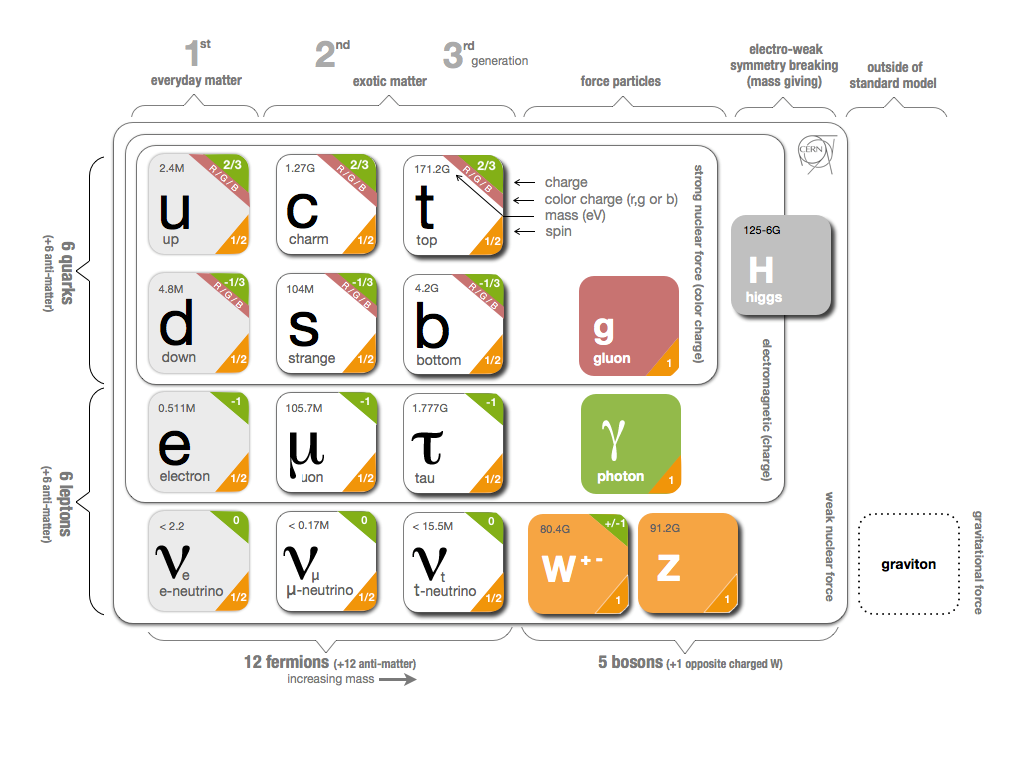
\includegraphics[width=0.8\textwidth]{Standard_model_infographic}
\caption{The fundamental particles in the Standard Model \cite{SMchart}.}
\label{fig:SMchart}
\end{figure}

The particles, listed in Fig.~\ref{fig:SMchart} can be divided in two classes:
fermions with an intrinsic spin of 1/2 make up everything that is usually called
``matter'', and exchange bosons with integer (1 in most cases) spin that convey
the interactions and couple to the respective charge. Formally, the bosons are
the generators of the gauge symmetry group of the particular interaction.

This means that the strong force, which obeys a \emph{SU(3)} symmetry, has eight
generators that are represented by eight gluons $g$. The gluons couple to the
strong charge which is usually referred to as ``colour''. Since it has the
largest coupling constant, the strong interaction is dominant whenever a
colour charge is present. However colour is ``confined'', i.e. free particles
must not have a net colour. This means that any coloured particles have to be
bound inside a compound object at all times. Also, the range of the strong
interaction is limited to about the size of a nucleus since the gluons are
coloured themselves and hence self-coupling.

About two orders of magnitude weaker is the electromagnetic interaction.
According to its \emph{U(1)} symmetry, it has only one exchange boson, the
photon $\gamma$, coupling to the electrical charge. It is massless and
electrically neutral, hence the electromagnetic interaction is not restricted
in range. This and the fact that there is no confinement on the electrical
charge mean that on macroscopic scales electromagnetic phenomena are dominant.

At low energies, the effective coupling constant of the weak interaction is
another three orders below the electromagnetic one. From its \emph{SU(2)}
symmetry originate three exchange bosons, $W^\pm$ and $Z^0$ with masses of
about 90\,MeV limiting its range to the subatomic scale. However with increasing
energy, the mass of the gauge bosons becomes more and more negligible and the
effective coupling rises. Above the electroweak unification at about 100\,GeV,
the weak and electromagnetic interactions can be described by one unified
theory, whose existence is also hinted to by the fact that the weak gauge
bosons are electrically charged.

Their masses arise from another spontaneously
broken local \emph{SU(2)}$\times$\emph{U(1)} symmetry of the so-called
Higgs\footnote{After Peter Higgs, who, together with others, laid the
foundations of this theory in the 1960's \cite{Higgs, BroutEnglert}.} field.
After breaking, the generators of the \emph{SU(2)} part mix with the weak
bosons, giving them mass, while the generator of the remaining \emph{U(1)} can
be observed as the only scalar gauge boson, the Higgs boson. The Higgs boson
was the last fundamental particle of the standard model to be detected, its
discovery was claimed by the ATLAS and CMS collaborations in 2012
\cite{AtlasHiggs, CMSHiggs}.

The other group of fundamental particles are the fermions (and their
corresponding antiparticles). They can be divided again into two subclasses: the
six quarks $u,\ d,\ c,\ s,\ t$, and $b$, which obey all forces and---being
coloured---are confined, so that no free quarks can be found in nature. Bound
quarks are making up baryons, like protons and neutrons, consisting of three
quarks, and unstable mesons, which consist of a quark and an antiquark, like
pions. Baryons and mesons, together called hadrons, are the only free particles
participating in the strong interaction, since they contain coloured quarks,
although not being coloured themselves.

The second subclass are the leptons, the three charged leptons $e$, $\mu$, and
$\tau$, as well as the corresponding (neutral) neutrinos \nue, \numu, and
\nutau. The charged leptons interact predominantly electromagnetically, most
prominently electrons are bound to nuclei via electrical attraction. However
the decay of $\mu$ and $\tau$ is---like every flavour-changing process---a weak
interaction. The electron as the lightest charged lepton has to be stable due
to conservation of energy and charge.

Since neutrinos are neither coloured nor electrically charged, they only
interact weakly. This means that they are very hard to detect directly. In
fact, their existence had already been suggested in 1930 by Wolfgang Pauli as a
solution for the problem of missing energy in radioactive $\beta$ decays
\cite{PauliBeta}. However the first direct detection of (electron) neutrinos,
\nue, from a nuclear reactor was achieved only in 1956 in the so-called
Cowan-Reines experiment \cite{CowanReines}. The existence of a second neutrino,
the muon neutrino \numu, was established few years later in 1962 from the study
of charged pion decays \cite{NuMuDiscovery}. The third neutrino, the \nutau,
was finally discovered directly by the DONUT experiment in 2001 in the decay of
$D_S$ mesons into \nutaubar and $\tau$, which again decay into \nutau and other
leptons \cite{DONUT}.

In addition to having neither colour nor electrical charge, the standard model
also predicts that neutrinos are massless. Thus the observation of neutrino
oscillations by the Super-Kamiokande experiment in 1998\footnote{Hints of
neutrino oscillations had already been observed in the 1960's
\cite{DaviesNuOsc}, but were widely refused by the scientific community.}
\cite{SuperKosc} gained much attention, this being the first detection of
physics beyond the standard model.

The term ``neutrino oscillations'' describes the phenomenon that neutrinos,
when propagating over macroscopic distances, can change their flavour
eigenstate on the way between production detection. The details of this effect
will be described in Sec.~\ref{sec:osc}. However it can only occur when there
are different mass eigenstates available for the neutrinos, meaning that only
one of them---if any---can have mass zero, while the others must correspond to
finite mass.

Since their first observation, neutrino oscillations have been a field of
intensive research. After establishing all oscillation channels, nowadays the
precise measurement of the parameters that characterise the oscillation is in
the focus. The planned PINGU experiment (see Sec.~\ref{sec:PINGU}), whose
simulation is the main topic of this thesis, is aimed to reach unprecedented
accuracy in measuring the parameters \thet{23} and \dm{31}.


\subsection{Neutrino Sources}
\label{sec:NuSources}

As discussed above, neutrinos do not participate in the strong and
electromagnetic interaction, leaving only weak processes for them to be created
or detected. On the other hand, neutrinos are produced in nearly every weak
interaction, making them a very common particle that can stem from a variety of
different sources in very different energy ranges.

\subsubsection{Natural Radioactivity}
On Earth, the most common source is the $\beta$ decay of natural radionuclides.
Depending on the type of the decay ($\beta^+$ or $\beta^-$), an electron
(anti-) neutrino is emitted along with the charged lepton. The general
equations read:
\begin{eqnarray}
 \beta^+: & ^A_Z\mathrm{X} & \to\quad  ^A_{Z-1}\mathrm{Y} + e^+ + \nue \\
 \beta^-: & ^A_Z\mathrm{X} & \to\quad  ^A_{Z+1}\mathrm{Y} + e^- + \nuebar
\end{eqnarray}
Examples for typical $\beta$ emitters are $^{40}$K (both $\beta^+$ and
$\beta^-$) and intermediate products from the decay chains of $^{232}$Th or
$^{238}$U ($\beta^-$), the neutrino energies are usually on the scale of few
MeV.

In fact, the $\beta$ decay was the original reason to propose the existence of
the then un-detectable neutrino. Since only the daughter nucleus and the
charged lepton were visible as decay products, the process seemed to be a
two-body decay. This means that the energies of the decay products are exactly
determined from kinematics and hence the emitted electrons or positrons would
be monoenergetic. Observations showed, however, a broad spectrum in energy
instead of a single line. Without violating the conservation of energy, this
can only be achieved if a third particle is produced in the process, which is
electrically neutral but can carry away energy and momentum. 

On the subatomic level, in a $\beta^+$ decay one proton inside a nucleus emits a
virtual $W^+$ boson, turning an $u$ into a $d$ quark, and becomes a neutron.
During a $\beta^-$ decay, the opposite happens via the emission of a $W^-$, as
shown in Fig.~\ref{fig:beta_minus}. The $W$ boson subsequently decays into a
charged lepton and a neutrino.

\begin{figure}
 \centering
 \begin{fmffile}{beta_minus}
 \begin{fmfgraph*}(80,50) \fmfpen{thin}
 \fmfstraight
  \fmfleft{i0,i1,i2,i3,i41,i42,i5,i51,i6}
  \fmfright{o0,o1,o2,o3,o41,o42,o5,051,o6}
  \fmf{fermion}{i0,o0}
  \fmflabel{$u$}{i0}
  \fmflabel{$u$}{o0}
  \fmf{fermion}{i1,o1}
  \fmflabel{$d$}{i1}
  \fmflabel{$d$}{o1}
  \fmf{fermion}{i2,v1,o2}
  \fmflabel{$d$}{i2}
  \fmflabel{$u$}{o2}
  \fmffreeze
  \fmf{fermion}{o5,v2,o6}
  \fmflabel{$e^-$}{o6}
  \fmflabel{\nuebar}{o5}
  \fmf{dashes,lab=$W^-$,l.side=left,tension=1.5}{v1,v2}
 \end{fmfgraph*}
 \end{fmffile}
 \write18{mpost beta_minus}
\caption{Feynman diagram of a $\beta^-$ decay}
\label{fig:beta_minus}
\end{figure}

% TODO: say something about 0n2b decay?


\subsubsection{Nuclear Reactors}

In nuclear reactors, the controlled fission of heavy elements is used for the
generation of electrical power. The intermediate products of these nuclear
fissions are unstable isotopes that usually have a large surplus of neutrons
compared to a stable configuration. These unstable nuclides undergo a series of
$\beta^-$ decays until they they reach a stable ratio of proton and neutron
numbers.

Since in each of those $\beta$ decays neutrinos are emitted, a nuclear reactor
provides a strong and steady flux of \nuebar, which can be monitored via the
thermal power of the reactor. This makes reactor neutrinos a popular target for
experiments, especially for the study of neutrino oscillations. The main
challenge in such experiments is the accurate modelling of the neutrino energy
spectrum, which is the sum of the spectra of all of the different $\beta$
decays in the decay chain. Even though there are very elaborate flux models
available, there might still be components unaccounted for, resulting in
unexpected features in the measured neutrino flux \cite{RENO_5MeV}.


\subsubsection{Neutrino Beams}

Another artificial source of neutrinos, but somewhat higher in energy
(typically at a few GeV) are neutrino beams. Since the neutral neutrinos cannot
be accelerated directly, usually a high-energy, high-intensity proton beam is
aimed at a target in which it produces mesons, mostly pions and kaons, in whose
subsequent decay neutrinos are produced \cite{NuBeams}:
\begin{eqnarray}
 \pi^+ & \to & \mu^+ + \numu \\
 \pi^- & \to & \mu^- + \numubar
\end{eqnarray}

Such beams are the source of neutrinos that can be controlled best in terms of
energy and intensity, making them a preferred choice for precision experiments
such as measurements of neutrino cross-sections. However they are very expensive
to build and operate in contrast to natural sources or nuclear reactors, the
latter usually being operated by commercial power suppliers.


\subsubsection{Solar Neutrinos}

In terms of total flux, the strongest source of neutrinos on Earth is the Sun.
In its interior, hydrogen is fused to helium mostly in the so-called pp
chain\footnote{Other fusion processes such as the CNO cycle and the production
of heavier elements are strongly suppressed since they need extremely high
pressures that the Sun cannot supply due to its comparatively low mass.},
producing the energy that powers the Sun's radiation\cite{RolfsRodney}.

\begin{figure}
\centering
  \subfloat[The different branches of the pp chain.
    ``Lost'' energy is not dissipated into the Sun, but carried away by
    neutrinos. \label{fig:pp_network}]
    {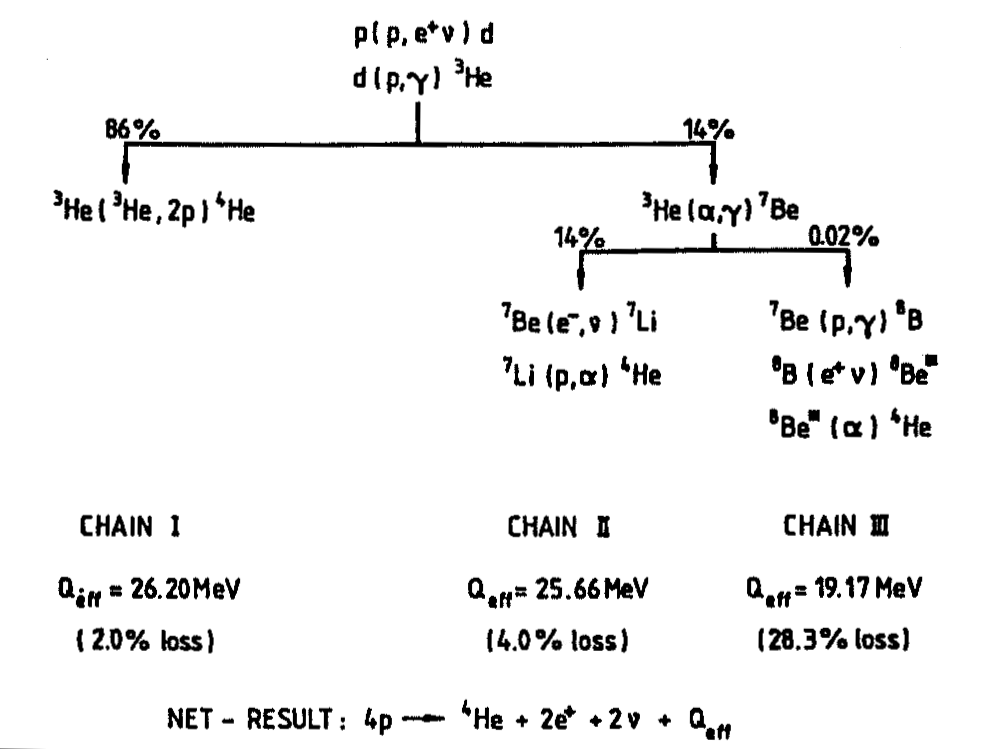
\includegraphics[width=0.45\textwidth]{pp_chain}}\qquad
  \subfloat[The solar neutrino spectrum from the pp chain.
    The neutrino fluxes are in units of cm$^{-2}$\,s$^{-1}$\,MeV$^{-1}$ for
    continuous and cm$^{-2}$\,s$^{-1}$ for discrete components.
    \label{fig:solar_nu_spectrum}]
    {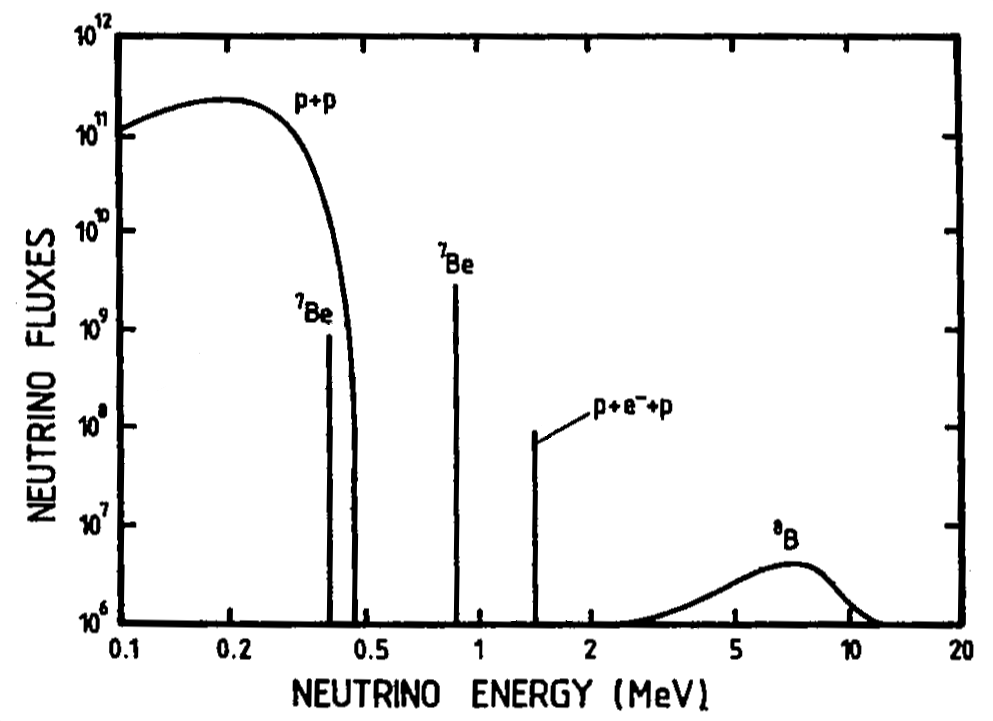
\includegraphics[width=0.45\textwidth]{solar_nu_spectrum}}
  \caption{The reactions and resulting neutrino spectrum of the solar pp chain.
    Figures adopted from \cite{RolfsRodney}.}
\label{fig:solar_nus}
\end{figure}

Effectively, this is carried out via the reaction
\begin{equation}
 4 p \to\ ^4_2\mathrm{He} + 2 e^+ + 2 \nue + 26.73\,\mathrm{MeV}\quad.
\end{equation}
In reality, this will not occur in a single step since it is a weak interaction
(as neutrinos are produced in its course) with a correspondingly small
cross-section which in addition has to overcome the Coulomb repulsion of the
four protons. Instead the fusion process involves several intermediate stages,
the first of which is the fusion of two protons to a deuteron,
\begin{equation}
 p + p \to\ d + e^+ + \nue\quad,
\end{equation}
releasing 0.42\,MeV of energy carried by the (subsequently annihilating)
positron and the so-called pp neutrino. The low Q value along with the
aforementioned low cross-section and Coulomb repulsion are the reason for the
long lifetime of free protons inside the Sun\footnote{And hence also the
long lifetime of the Sun itself}---it takes them an average of about $10^{10}$
years to fuse to deuterium. A competing, but even more improbable reaction is
the pep process, where an electron is involved directly in the fusion and no
positron is produced:
\begin{equation}
 p + e^- + p \to\ d + \nue
\end{equation}
Since there are only two particles in the final state, the produced neutrinos
are monoenergetic at 1.44\,MeV. Once a deuteron is produced, it quickly (YYY\,s)
merges with another proton to $^3_2\mathrm{He}$ and emits a photon.

At this stage, the pp chain divides into three different branches (see
Fig.~\ref{fig:pp_network}). In the main branch, ppI, two $^3_2\mathrm{He}$
nuclei fuse to $^4_2\mathrm{He}$, also called an $\alpha$ particle, and two
protons that can then enter the pp chain again. However in terms of neutrinos,
the two subdominant branches ppII and ppIII are much more interesting,
especially since the pep and pp neutrinos, who make up the main part of the
solar neutrinos, are very low in energy and thus difficult to detect.

If a $^3_2\mathrm{He}$ does not fuse with another $^3_2\mathrm{He}$, but with
a $^4_2\mathrm{He}$ instead, $^7_4\mathrm{Be}$ is formed. In most cases, this
will then capture an electron to produce $^7_3\mathrm{Li}$ under the emission
of a neutrino in the ppII branch:
\begin{equation}
 ^7_4\mathrm{Be} + e^- \to\ ^7_3\mathrm{Li} + \nue
\end{equation}
These so-called $^7$Be neutrinos have an energy of 0.86\,MeV. Due to this high
energy and their rather high flux portion of about 14\,\%, they were targeted
in the first detection of solar neutrinos \cite{DaviesNuOsc}. The
$^7_3\mathrm{Li}$ finally catches another proton to form two $^4_2\mathrm{He}$
nuclei.

Sometimes, the $^7_4\mathrm{Be}$ reacts with a proton rather than an electron
(ppIII branch) and forms $^8_5\mathrm{B}$, which is a $\beta^+$ emitter with a
half-life of 0.77\,s \cite{Nuklidkarte}. Although their flux is very low, the
very high Q-value of 14.1\,MeV of this decay makes the so-called $^8$B a
favourable target for the search for solar neutrinos.

The excited $^8_4\mathrm{Be}$ created in the decay
\begin{equation}
 ^8_5\mathrm{B} \to\ ^8_4\mathrm{Be^*} + e^+ + \nue
\end{equation}
will then further decay into two $\alpha$ particles immediately.


\subsubsection{Atmospheric Neutrinos}
\label{sec:AtmNus}

Several orders of magnitude higher in energy are neutrinos that are created in
the interaction of high-energy charged particles with atoms in the Earth's
atmosphere. During the past decades, the spectrum of these particles, the 
so-called cosmic radiation, has been measured in great detail over many orders
of magnitude. Although it covers such a wide range in energy and flux, it shows
almost no features and can be described by a simple power law with a spectral
index of $\gamma=-2.7$, softening to $\gamma=-3.0$ at the so-called ``knee'' at
a few PeV and turning back to $\gamma=-2.7$ at the ``ankle'' at the highest
energies \cite{CosmRad}.

\begin{figure}
\centering
  \subfloat[The all particle spectrum of the charged cosmic radiation. Figure
    taken from \cite{CosmRaySpec}. \label{fig:CosmRaySpec}]
    {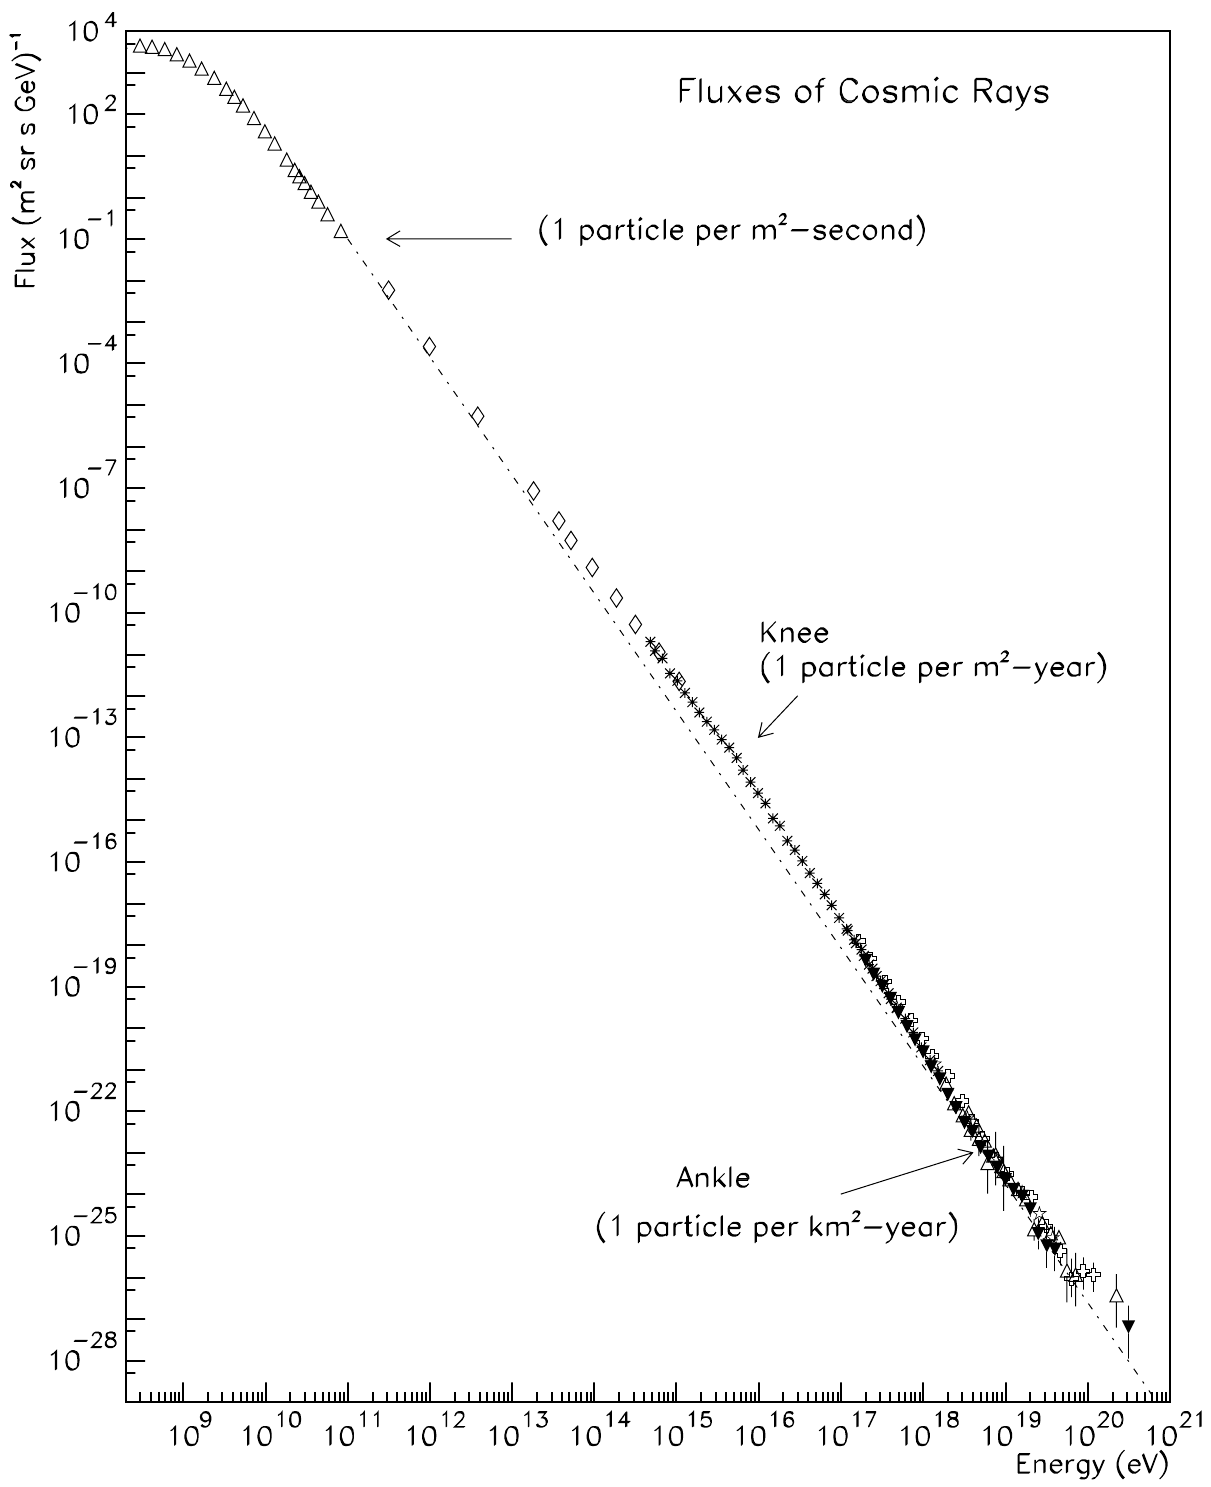
\includegraphics[height=7cm]{CosmicRaySpectrum}}\qquad
  \subfloat[The atmospheric flux of electron and muon neutrinos.
    Predictions for the conventional flux are from \cite{Honda2007} (solid
    lines) and \cite{Bartol} (dashed), the band for the prompt flux is
    according to \cite{PromptFlux}. Figure taken from \cite{IC_AtmCscd}.
    \label{fig:AtmFlux}]
    {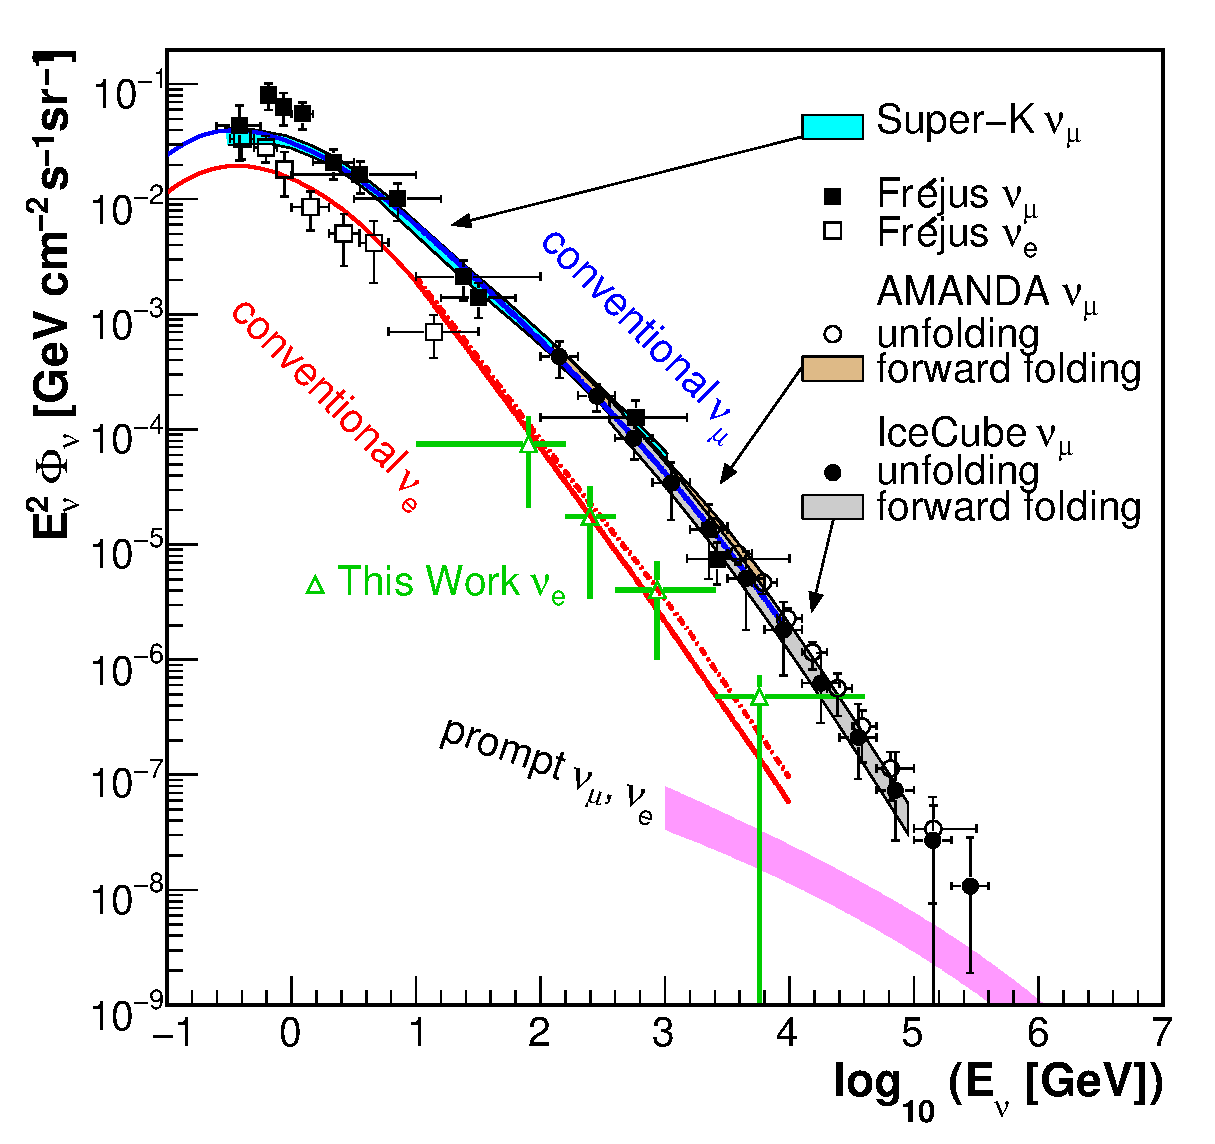
\includegraphics[height=7cm]{AtmFlux}}
  \caption{Spectra of the cosmic radiation at Earth and the resulting
    atmospheric neutrino spectrum.}
\label{fig:cosmic_rays_atm_nus}
\end{figure}

The origin of the cosmic radiation is not fully established yet. However it is
commonly assumed that the particles are accelerated in non-thermal processes,
usually moving shock fronts, that develop in extreme astrophysical environments.
This mechanism is known as Fermi acceleration \cite{FermiAcc}. 
Candidates for the acceleration sites are both galactic sources, such as
supernova remnants, as well as extragalactic ones like gamma ray bursts or
active galaxies. Due to their small size and rather low energy density, galactic
sources are believed to dominate the low-energy part of the spectrum in the GeV
to TeV regime, while the extragalactic contribution takes over at the knee
region.

When such a high energy particle hits the Earth's atmosphere, it interacts with
a nucleus in the air (usually nitrogen or oxygen) in a so-called deep-inelastic
scattering process. Since the energy of the incoming particle is far beyond all
binding energies in the nucleus, it is completely disrupted. From the fragments
of the nucleus that are still highly energetic, a shower of secondary particles
develops, that then travels down to Earth.

Main components of these particle showers are muons and pions. Both particles
are relatively short-lived\footnote{$\tau_\mu = 2.2 \times 10^{-6}$\,s and
$\tau_\pi = 2.6 \times 10^{-8}$\,s \cite{PDG}} and produce neutrinos in their
decay:
\begin{eqnarray}
 \pi^\pm &\to\ & \mu^\pm + \numu(\numubar) \\
 \mu^\pm &\to\ & e^\pm + \nue(\nuebar) + \numubar(\numu)
 \label{eqn:pi_decay}
\end{eqnarray}
As one can see from the above equations, these so-called conventional
atmospheric neutrinos coming mostly from pion decay have a flavour ratio of
$\overset{(-)}{\numu}:\overset{(-)}{\nue} = 2:1$.

Their energy spectrum is linked to the primary spectrum of cosmic rays since the
secondary pions and muons follow the primary energy distribution directly. Thus
being highly relativistic, their lifetime is Lorentz boosted by a factor $\gamma
\propto E$. This means that the higher the pion's (or muon's) energy, the higher
its probability \emph{not} to decay into neutrinos in-flight but reach the
Earth's surface and interact there, producing another shower of much less
energetic particles. Hence the spectrum of conventional atmospheric neutrinos
is suppressed roughly by a factor of $1/E$ with respect to the primary cosmic
ray distribution.

For a more precise calculation, details of high-energy proton interactions and
the geomagnetic field have to be taken into account \cite{Honda2007, Bartol}. As
shown in Fig.~\ref{fig:cosmic_rays_atm_nus}, these predictions show good
agreement with measurements.

Another predicted, but not yet observed component of the atmospheric neutrino
flux are the so-called prompt neutrinos. They originate from charmed mesons,
mostly kaons, that are rarely produced in cosmic ray induced air showers as
well. Since these are so short-lived that they always decay in-flight
(``promptly'') despite of their relativistic boost, their energy spectrum
is the same as the primary one and thus harder than the conventional component,
but with a much smaller normalisation.

\subsubsection{Supernova Neutrinos}
% TODO: mention them?

\subsubsection{Astrophysical Neutrinos}

The highest energy neutrinos are the so-called astrophysical ones. They are  
assumed to be produced at similar sites as the cosmic radiation, i.\,e.\ in 
highly energetic shock fronts. There, $\Delta$ resonances are generated in the 
collision of protons and high-energy photons, producing pions in their decay:
\begin{equation}
 p + \gamma \to \Delta^+ \to n + \pi^+\ (p + \pi^0)
\end{equation}
The pions then decay further into neutrinos as shown in (\ref{eqn:pi_decay}).

Since astrophysical neutrinos are produced in the same processes as cosmic 
rays, their fluxes are linked. The flux of cosmic rays has been measured in 
quite some detail over the recent decades \cite{CosmRaySpec}, hence an upper 
limit for the flux of astrophysical neutrinos can be derived that is 
independent of any model assumptions about the production sites \cite{WB_bound}.

The first actual astrophysical neutrino events have been recorded only recently 
by the IceCube neutrino telescope \cite{HESE, HESE_3yr}, making them the 
highest energy neutrinos ever observed. Although event statistics are still 
low, the flux seems to be very close to the predicted upper bound, meaning that 
the neutrino production efficiency is close to maximal. The spectral shape of 
the flux is compatible with a power law with an index of --2 and an exponential 
cut-off around a few PeV \cite{Lars_globalfit}.

\subsection{Detection of Neutrinos}

As already mentioned, neutrinos only interact with other particles in weak
processes. This means that the total cross-sections are typically low. So high
fluxes or large target volumes (or both) are needed to detect a seizable
number of neutrinos.

And even if these requirements are fulfilled, in most cases the neutrino signal
has to be recovered from below a background of dominant processes, whose rate
can be several orders of magnitude higher than the neutrino event rate.
Depending on the targeted energy range, the most common background processes are
inherent radioactivity of the surroundings and the detector itself at MeV
energies, and muons created in cosmic ray induced air showers which can
penetrate even strong shielding.

\subsubsection{Neutrino cross-sections}

\begin{figure}
 \centering
 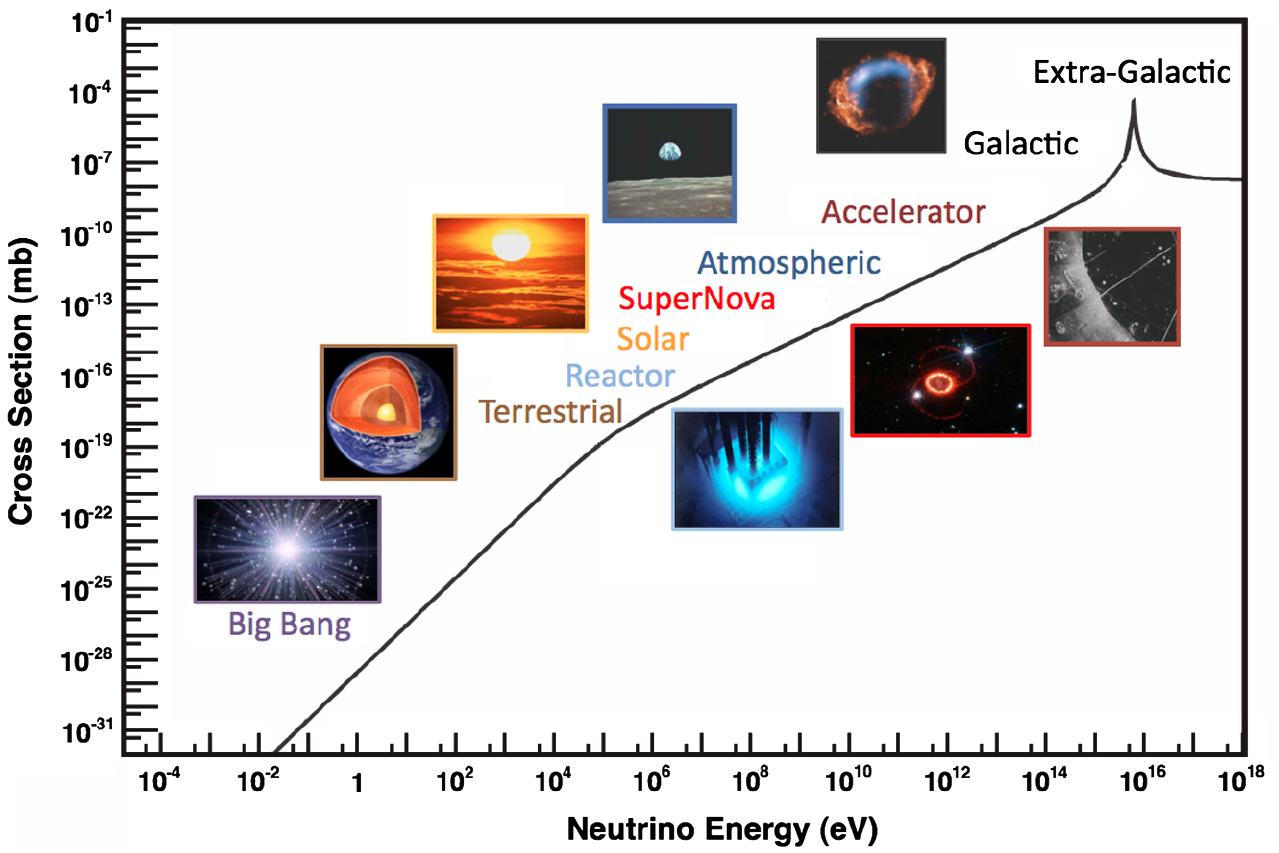
\includegraphics[width=0.7\textwidth]{NuXsec_fullrange}
\caption{Electroweak cross-section for $\nue e^- \to \nue e^-$ scattering
  on free electrons as a function of neutrino energy. Various neutrino sources
  are also shown at their respective energy scales. \cite{NuXsec_review}}
 \label{fig:nue_e_xsec}
\end{figure} 

The calculation and experimental testing of neutrino cross-sections has been a
field of extensive research over the past decades. On the experimental side,
the challenge is the smallness of the cross-sections. The key point on the
theoretical side is the calculation of the matrix elements associated with the
interaction of interest.

As an introductory example, we will look at neutrinos scattering off a free
lepton. Then the cross-section is \cite{NuXsec_review}
\begin{equation}
 \frac{d\sigma}{dq^2} = \frac{1}{16\pi} \frac{|\mathcal{M}^2|}{(s-m_e^2)^2}\ ,
\end{equation}
with $s$ and $q^2$ being the centre-of-mass energy and the four-momentum
transfer, respectively, assuming very small neutrino mass. In this case,
calculating the matrix element $|\mathcal{M}^2|$ is rather straightforward,
since only weak interactions between fundamental particles have to be
considered. The scattering process itself is the sum of a charged-current
($W^+$ exchange, CC) and a neutral current ($Z^0$ exchange, NC) contribution, as
shown in Fig.~\ref{fig:nue_e_CC}.

% TODO: Feynman graphs!
\begin{figure}
 \centering
 \begin{fmffile}{nue_e_CC}
 \parbox{50mm}{
  \begin{fmfgraph*}(40,30) \fmfpen{thin}
    \fmfstraight
    \fmfleft{i00,i0,i2,i3,i41,i42,i5,i51,i6,i1}
    \fmfright{o00,o0,o2,o3,o41,o42,o5,o51,o6,o1}
    \fmf{fermion}{i0,v0,o0}
    \fmflabel{$e^-$}{i0}
    \fmflabel{$\nue$}{o0}
    \fmf{fermion}{i1,v1,o1}
    \fmflabel{$\nu_f$}{i1}
    \fmflabel{$f^-$}{o1}
    \fmf{dashes,lab=$W$,l.side=left,tension=1.}{v0,v1}
  \end{fmfgraph*}
  } + \qquad \quad
 \parbox{50mm}{
  \begin{fmfgraph*}(40,30) \fmfpen{thin}
    \fmfstraight
    \fmfleft{i00,i0,i2,i3,i41,i42,i5,i51,i6,i1}
    \fmfright{o00,o0,o2,o3,o41,o42,o5,o51,o6,o1}
    \fmf{fermion}{i0,v0,o0}
    \fmflabel{$e^-$}{i0}
    \fmflabel{$f^-$}{o0}
    \fmf{fermion}{i1,v1,o1}
    \fmflabel{$\nu_f$}{i1}
    \fmflabel{$\nue$}{o1}
    \fmf{dashes,lab=$Z^0$,l.side=left,tension=1.}{v0,v1}
  \end{fmfgraph*}
 }
 \end{fmffile}
 \write18{mpost nue_e_CC}
 \caption{Feynman diagrams for the charged (left) and neutral (right) current
  contributions of $\nu_f\,e^- \to \nue\,f^-$ scattering.}
\label{fig:nue_e_CC}
\end{figure}

After converting from momentum transfer to the energy fraction $y$ carried by 
the outgoing lepton, $\frac{dq^2}{dy} = 2m_e E_\nu$, the charged current
cross-section for scattering off an electron is given by \cite{NuXsec_review}
\begin{equation}
 \frac{d\sigma}{dq^2}\bigg\rvert_\mathrm{CC} = \frac{2m_e G_F^2 E_\nu}{\pi}
  \left(1 - \frac{m_f^2 - m_e^2}{2m_e E_\nu}\right)\ ,
 \label{eqn:nue_e_xsec}
\end{equation}
where $E_\nu$ is the incoming neutrino energy, and $m_e$ and $m_f$ are the
masses of the electron and the outgoing fermion. The corresponding total
cross-section for $\nue e^- \to \nue e^-$ scattering is shown in
Fig.~\ref{fig:nue_e_xsec}. In case that $m_f$ can be neglected compared to the
neutrino energy, the above can be integrated to give a simple expression for
the total cross-section:
\begin{equation}
 \sigma \simeq \frac{2m_e G_F^2 E_\nu}{\pi} = \frac{G_F^2 s}{\pi}
\end{equation}
In Fig.~\ref{fig:nue_e_xsec}, this corresponds to the regime above about
$10^7$\,eV, well above the electron mass. The sharp peak at $\sim 10^{16}$\,eV
is the so-called Glashow resonance, where the centre-of-mass energy is
comparable to the $W$ boson mass, enabling resonant production of real $W^-$
bosons and hence causing a strong enhancement of the cross-section.

% FIXME: also write down nubar  and NC cross-section?

When looking at other scattering processes, the principles of deriving the
cross-section remain the same. However the kinematic part is subject to change,
mostly due to different angular momentum states, and of course the matrix
elements depend strongly on the respective target. For non-fundamental targets,
form factors describing their internal charge distribution have to be taken
into account as well.

In general, the cross-section for hadronic interactions are much larger than the
leptonic ones (e.\,g.\ neutrino-electron scatting as discussed above) due to the
larger target masses. This means that for conventional target consisting of
atoms with a nucleus and an electron hull, a neutrino is much more likely to
interact with the nuclei than with the shell electrons.

\subsubsection{Neutrino interactions with hadrons at the GeV scale}

\begin{figure}
\centering
  \subfloat
    {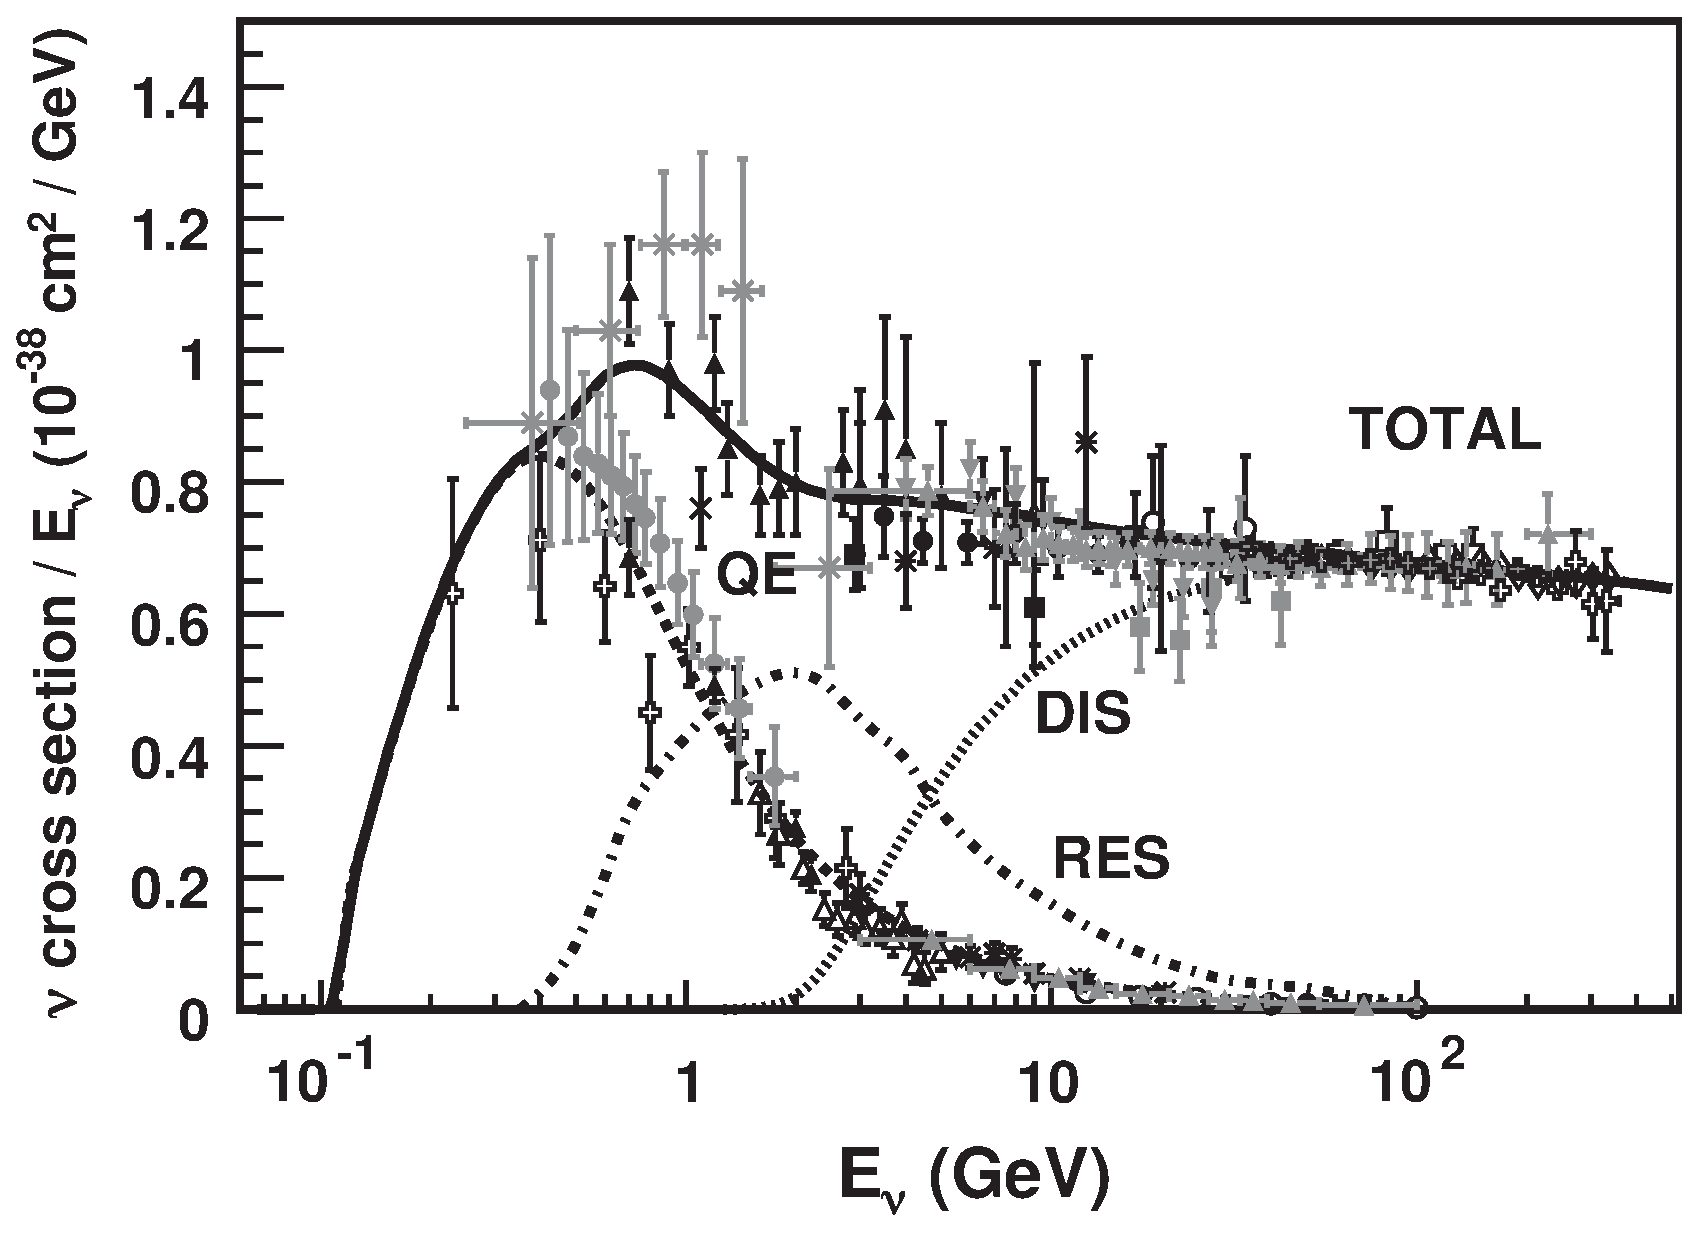
\includegraphics[width=7cm]{nu_N_xsec}}\qquad
  \subfloat
    {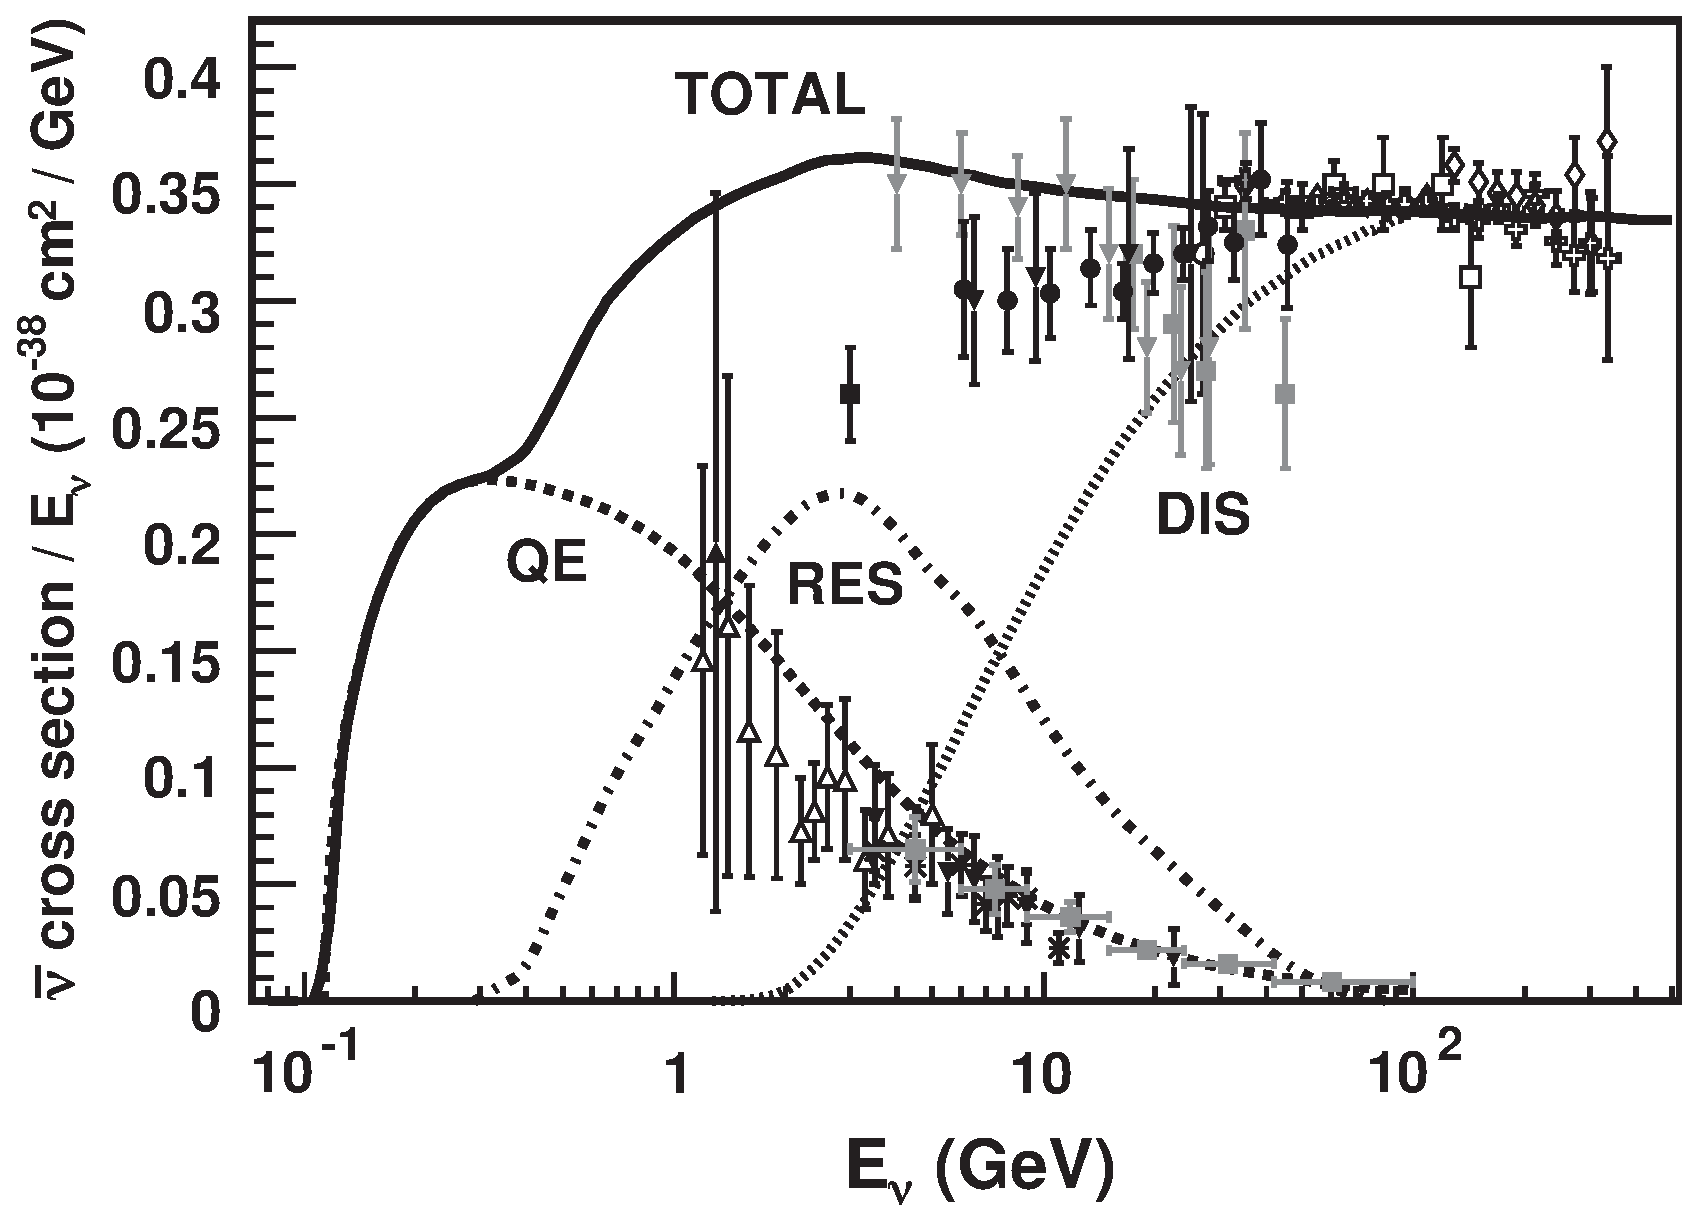
\includegraphics[width=7cm]{nubar_N_xsec}}
  \caption{Total CC cross-section for neutrino (left) and antineutrino
   (right) cross-section for an isoscalar nucleon, $N=(p+n)/2$, divided by the
   neutrino energy and plotted as a function of energy. Shown are data from
   various experiments and predictions for the quasi-elastic (QE), resonance
   (RES), and deep inelastic (DIS) contributions \cite{NuXsec_review}.}
\label{fig:NuXsec_GeV}
\end{figure}

For the scope of this thesis, the most interesting energy regime is the low GeV
scale, especially the range of $1 - 50$\,GeV. Here the cross-section for
neutrino interactions with nuclei is quite complex to describe, as several
distinct processes (shown in Fig.~\ref{fig:NuXsec_GeV}) have to be considered
for the scattering:
\begin{itemize}
 \item \emph{Quasi-elastic scattering:} At rather low energies, the neutrino
    scatters off an entire nucleon, removing it (possibly together with other
    nucleons) from the nucleus. The free proton(s) or neutron(s) will then
    propagate through the surrounding medium until they have dissipated all
    their energy. These interactions range out quickly above about 10\,GeV.
 \item \emph{Resonance production:} At the range of about $1-3$\,GeV, the
    dominant process is the excitation of short-lived baryonic resonances
    (such as $\Delta^+$ or $N^*$) in the target nucleon. These resonances then
    decay to various final states producing nucleons and $\pi$ mesons.
 \item \emph{Deep inelastic scattering:} Above about 10\,GeV, the scattering
    neutrino has sufficient energy to resolve the quark structure of the
    nucleons. Then it scatters on a quark constituent rather than the whole
    nucleon. By this, the nucleon gets disrupted and an hadronic shower
    consisting of a variety of mesons forms from its remains.
\end{itemize}

Common to all these processes is that they have both a CC and a NC
contribution---similar to the scattering off electrons shown in
Fig.~\ref{fig:nue_e_CC}, only that the target is either a whole (for
quasi-elastic and resonant processes) or a quark inside a nucleon (deep
inelastic scattering).

\begin{figure}
 \centering
 \begin{fmffile}{nux_NC}
 \begin{fmfgraph*}(50,30) \fmfpen{thin}
 \fmfstraight
  \fmfleftn{i}{8}
  \fmfrightn{o}{8}
  \fmf{heavy}{i2,v1}
  \fmfv{decor.shape=circle,decor.filled=shaded}{v1}
  \fmf{vanilla}{v1,o2}
  \fmflabel{nucleus}{i2}
  \fmflabel{hadronic\ shower}{o2}
  \fmf{fermion}{i8,v2,o8}
  \fmflabel{$\nu$}{i8}
  \fmflabel{$\nu'$}{o8}
  \fmf{dashes,lab=$Z^0$,l.side=left,tension=1.5}{v1,v2}
  \fmffreeze
  \fmf{vanilla}{v1,o1}
  \fmf{vanilla}{v1,o3}
 \end{fmfgraph*}
 \end{fmffile}
 \write18{mpost nux_NC}
\caption{Neutral current interaction between a neutrino and a nucleus.}
\label{fig:nux_NC}
\end{figure}

From the detection point of view, this means that there are four classes of
events. The first are neutral current interactions of any neutrino flavour, as
shown in Fig.~\ref{fig:nux_NC}. In this case, we have in the final state the
scattered neutrino $\nu'$ and a hadronic shower or cascade consisting
of a variety of mesons, fermions, and photons developing from the fragments of
the stricken nucleus.

The details of the development of such a hadronic shower are not fully
understood and have to be modelled in MonteCarlo based simulations. However,
since the involved particles are mostly short-lived and strongly interacting,
the typical size is on the order of one meter or below. 

The outgoing neutrino on the other hand is virtually impossible to detect,
meaning that the fraction of the total interaction energy that is carried by
this neutrino remains invisible. In beam experiments, where the energy of the
incoming particles is known, this is commonly referred to as ``missing energy''.

\begin{figure}
\centering
  \subfloat[\label{fig:nue_CC}]
    {
     \begin{fmffile}{nue_CC}
      \begin{fmfgraph*}(30,20) \fmfpen{thin}
      \fmfstraight
        \fmfleftn{i}{8}
        \fmfrightn{o}{8}
        \fmf{heavy}{i2,v1}
        \fmfv{decor.shape=circle,decor.filled=shaded}{v1}
        \fmf{vanilla}{v1,o2}
        \fmf{dashes,lab=$W$,l.side=left}{v1,v2}
        \fmf{fermion}{i7,v2}
        \fmflabel{\nue}{i7}
        \fmf{phantom}{v2,o7}
        \fmffreeze
        \fmf{fermion,lab=$e$,l.side=left,tension=2}{v2,v3}
        \fmf{vanilla}{v3,o7}
        \fmflabel{EM\ shower}{o6}
        \fmf{vanilla}{v1,o1}
        \fmf{vanilla}{v1,o3}
        \fmf{vanilla}{v3,o6}
        \fmf{vanilla}{v3,o8}
      \end{fmfgraph*}
     \end{fmffile}
     \write18{mpost nue_CC}
    }\qquad\qquad
  \subfloat[\label{fig:numu_CC}]
    {
     \begin{fmffile}{numu_CC}
      \begin{fmfgraph*}(30,20) \fmfpen{thin}
      \fmfstraight
        \fmfleftn{i}{8}
        \fmfrightn{o}{8}
        \fmf{heavy}{i2,v1}
        \fmfv{decor.shape=circle,decor.filled=shaded}{v1}
        \fmf{vanilla}{v1,o2}
        \fmf{dashes,lab=$W$,l.side=left}{v1,v2}
        \fmf{fermion}{i7,v2,o7}
        \fmflabel{\numu}{i7}
        \fmflabel{$\mu$}{o7}
        \fmffreeze
        \fmf{vanilla}{v1,o1}
        \fmf{vanilla}{v1,o3}
      \end{fmfgraph*}
     \end{fmffile}
     \write18{mpost numu_CC}
    }\qquad\qquad
  \subfloat[\label{fig:nutau_CC}]
    {
     \begin{fmffile}{nutau_CC}
      \begin{fmfgraph*}(30,20) \fmfpen{thin}
      \fmfstraight
        \fmfleftn{i}{8}
        \fmfrightn{o}{10}
        \fmf{heavy}{i2,v1}
        \fmfv{decor.shape=circle,decor.filled=shaded}{v1}
        \fmf{vanilla}{v1,o2}
        \fmf{dashes,lab=$W$,l.side=left}{v1,v2}
        \fmf{fermion}{i7,v2}
        \fmflabel{\nutau}{i7}
        \fmf{phantom}{v2,o7}
        \fmffreeze
        \fmf{fermion,lab=$\tau$,l.side=left,tension=5}{v2,v3}
        \fmf{vanilla}{v3,o7}
        \fmflabel{hadr./EM\ shower}{o7}
        \fmf{vanilla}{v1,o1}
        \fmf{vanilla}{v1,o3}
        \fmf{vanilla}{v3,o6}
        \fmf{vanilla}{v3,o8}
        \fmf{fermion}{v3,o10}
        \fmflabel{\nutau}{o10}
      \end{fmfgraph*}
     \end{fmffile}
     \write18{mpost nutau_CC}
    }
  \caption{Charged current interactions between a \nue (a), \numu (b), and
           \nutau (c) and a nucleus.}
\label{fig:nu_CC}
\end{figure}

In charged current interactions, the neutrino scatters off a nucleus by
exchanging a $W$ boson. From the fragmented nucleus, a hadronic shower develops
similarly to the neutral current case. The outgoing lepton however is now a
charged one, the flavour corresponding to the incoming neutrino's flavour. This
charged lepton now dominates the event signature:

\begin{description}
 \item[Electron:] In dense matter, a GeV electron will trigger an
  electromagnetic shower by radiating high-energy photons (bremsstrahlung),
  which in turn will create electron-positron pairs. The typical scale length
  $X_0$ of such a shower is given by
  \begin{equation}
   \frac{1}{X_0} = 4\alpha r_e^2 \frac{N_A}{A}
                    \left\{ Z^2 \left[L_\mathrm{rad} - f(Z) \right]
                    + Z\,L_\mathrm{rad}'\right\} \quad,
   \label{eqn:rad_length}
  \end{equation}
  where $\alpha$ is the fine structure constant, $r_e$ the classical electron
  radius, and $N_A$ Avogadro's number. $A$ and $Z$ are atomic mass and charge
  of the medium, and $L_\mathrm{rad}$, $L_\mathrm{rad}'$, and $f(Z)$
  semi-empirical parameters that have been tabulated \cite{PDG, bremsstrahlung}.
  For water, the scale length is $X_\mathrm{0,\,H_2O} =
  24.33\,\mathrm{g/cm}^2$, meaning that the typical size of such a shower is
  about one meter, as water has a density of $\varrho_\mathrm{H_2O} =
  1$\,g/cm$^3$.
 \item[Muon:] In contrast to the much lighter electron, a muon of a few GeV is
  a so-called minimum ionising particle. This means it is in the minimum region
  of the Bethe-Bloch formula for the energy loss of a charged particle:
  \begin{equation}
   \left\langle -\frac{dE}{dx}\right\rangle = Kz^2\frac{Z}{A}\frac{1}{\beta^2}
      \left[ \frac{1}{2}\ln\frac{2m_ec^2\beta^2\gamma^2 W_\mathrm{max}}{I^2}
             - \beta^2 - \frac{\delta(\beta\gamma)}{2} \right] \quad.
   \label{eqn:bethe-bloch}
  \end{equation}
  Here, $K = 4\pi N_A r_e^2 m_ec^2$, $z=1$ is the electrical charge of the
  muon, $I$ the mean excitation potential of the material, $\delta(\beta\gamma)$
  a density effect correction, and $W_\mathrm{max}$  the maximum energy transfer
  in a single collision between the muon and an  electron in the medium.
  $\beta = v/c$ and $\gamma$ are the Lorentz variables \cite{PDG}.

  This expression has a wide minimum in the range $\beta\gamma\approx 1 - 100$, 
  corresponding to a muon momentum in the low GeV/$c$ regime. Here,
  (\ref{eqn:bethe-bloch}) evaluates to $\langle dE/dx\rangle \approx
  2$\,MeV/(g/cm$^2$), hence for a medium with a density of 1\,g/cm$^3$ a muon
  has a range of approximately 5\,m/GeV before it has deposited all its energy
  and decays at rest.
 \item[Tau:] In principle, a tau lepton is a minimum ionising particle as well.
  But with a lifetime of only $2.9\times10^{-13}$\,s and a mass of 1.78\,GeV, at
  GeV energies it can travel at most a few hundred microns before it decays. In
  its decay, a \nutau has to be created again, whose energy has to be considered
  ``missing'' again. The remaining decay products form an electromagnetic or
  hadronic shower, depending on their nature.
\end{description}

In a large detector with detection units spaced widely on a scale of several 
meters, the four event classes discussed above can only be categorized into two 
channels: tracks and cascades.


\subsubsection{Cherenkov effect}
%==============================================================================
\chapter{Neutrino Oscillations}
\label{sec:osc}
%==============================================================================

The Standard Model of Particle Physics, as described in the previous chapter,
has been one of the most successful theories in the history of physics. It is,
however, not fundamental in the sense that it can explain all physical
phenomena alone. Its shortcomings are e.\,g.\ the missing inclusion of the
fourth fundamental force, gravity, and a lack of explanation for the fundamental
asymmetry between bosons and fermions.
There are theoretical extensions to the Standard Model addressing these
questions, such as ``Grand Unified Theories'', supersymmetry, and many others 
\cite{Nagashima}, but all of them lack experimental evidence so far.

Yet there is one effect of so-called ``Physics beyond the Standard Model'' that
has been well established experimentally during the past years: neutrino
oscillations. As already mentioned in Sec.~\ref{sec:NusInSM}, this term refers
to neutrinos changing their flavour when travelling over macroscopic distances,
which can be explained by finite neutrino masses, while in the Standard Model
they have zero mass.

The theory behind this process will be described in the following. In-depth
treatments of this topic can be found in many textbooks, e.\,g.\
\cite{GiuntiKim, Zuber, Nagashima, XingZhou}. The notation will follow
\cite{GiuntiKim} here.

\section{Vacuum Oscillations}
\label{sec:VacOsc}

There are two bases of eigenstates to which a neutrino can be decomposed: the
flavour and the mass base. The flavour eigenstates are \ket{\nue}, \ket{\numu},
and \ket{\nutau}, which will be summarised as \ket{\nu_\alpha}. These are the
eigenstates of the weak interaction, hence neutrinos are always produced as a
pure flavour eigenstate and have to be projected back onto these eigenstates
whenever they interact.

On the other hand there are the three mass eigenstates \ket{\nu_1}, \ket{\nu_2},
and \ket{\nu_3}, summarised as \ket{\nu_k}, corresponding to the three neutrino
masses $m_k$. The absolute values of these masses are yet unknown, but since
neutrino oscillations have been observed, at least two of them have to be
different from zero. The mass eigenstates have to be considered when describing
the propagation of a neutrino in vacuum since they are the eigenstates of the
corresponding Hamiltonian
\begin{equation}
%  \hat{H} = -\frac{\hbar^2}{2m}\nabla^2
 \hat{H}\,\ket{\nu_k} = E_k\,\ket{\nu_k} \quad.
 \label{eqn:vac_hamiltonian}
\end{equation}
% only depends on its mass.

\subsection{General Case}

Changes between the two bases are carried out via the so-called PMNS
matrix\footnote{After Bruno Pontecorvo, Ziro Maki, Masami Nakagawa, and Shoichi
Sakata.} $\mathcal{U}_\mathrm{PMNS}$ that can be parametrised using three Euler
angles \thet{ij}, also called mixing angles, and one complex phase angle
$\delta$ that is related to possible CP violation:
\begin{equation}
 \mathcal{U}_\mathrm{PMNS} =
 \begin{pmatrix}
  U_{e1} & U_{e2} & U_{e3} \\
  U_{\mu 1} & U_{\mu 2} & U_{\mu 3} \\
  U_{\tau 1} & U_{\tau 2} & U_{\tau 3}
 \end{pmatrix}
 =
 \begin{pmatrix}
  1 & 0 & 0 \\
  0 & c_{23} & s_{23} \\
  0 & -s_{23} & c_{23}
 \end{pmatrix}
 \begin{pmatrix}
  c_{13} & 0 & s_{13}e^{-i\delta} \\
  0 & 1 & 0 \\
  -s_{13}e^{i\delta} & 0 & c_{13}
 \end{pmatrix}
 \begin{pmatrix}
  c_{12} & s_{12} & 0 \\
  -s_{12} & c_{12} & 0 \\
  0 & 0 & 1
 \end{pmatrix}
\label{eqn:PMNS}
\end{equation}
Here, $s_{ij}$ and $c_{ij}$ are shorthands for $\sin\thet{ij}$ and
$\cos\thet{ij}$, respectively. Transformations between flavour and mass base
are then given by
\begin{eqnarray}
 \ket{\nu_\alpha} = \sum_k U^*_{\alpha k}\, \ket{\nu_k}\quad, \\
 \ket{\nu_k} = \sum_\alpha U_{\alpha k}\, \ket{\nu_\alpha}\quad.
\end{eqnarray}

To ensure lepton number conservation, unitarity of $\mathcal{U}_\mathrm{PMNS}$
has to be required. Any deviation from this can be interpreted as a hint for
additional neutrino flavours that do not participate in the weak
interaction\footnote{Measurements of the $Z^0$ decay width have shown that only
three weakly interacting neutrino flavours exist \cite{Zwidth}---at least at
masses up to half the $Z^0$ mass, $m_\nu < m_{Z^0}/2 = 45.6$\,GeV.}. Such
signals have been reported (e.\,g.\ \cite{MiniBooNE}), but the overall
picture remains inconclusive \cite{PDG}.

% TODO: Make Hamiltonian matrix formalism more clear

If now a pure flavour eigenstate \ket{\nu_\alpha} is produced at an energy $E$,
the probability to detect it as \ket{\nu_\beta} after propagating over a
distance $L$ has to be calculated according to
\begin{equation}
 P_{\alpha\to\beta} = \left|\Braket{\nu_\beta
                            \left|\,\mathcal{U}^\dagger\,\left|\,\hat{H}
                             \,\right|\,\mathcal{U}\,\right|
                             \nu_\alpha}\right|^2 \quad.
 \label{eqn:osc_prob_hamiltonian}
\end{equation}
In the mass base, the propagation of the neutrinos can be described as plain
waves,
\begin{equation}
 \Ket{\nu_k(t)} = \exp\left(-i(E_k t - \vec{p}_k\cdot \vec{x})\right)\,
  \Ket{\nu_k(0)} \quad,
\end{equation}
and assuming relativistic neutrinos ($m_k \ll E_k \Rightarrow v \approx c$) one
can approximate in natural units\footnote{$\hbar = c = 1$}
\begin{eqnarray}
 E_k =       \sqrt{ \vec{p}_k^2 - m_k^2 }
     \approx p_k + \frac{m_k^2}{2p_k} \quad, \\
 E_k t - \vec{p}_k\cdot \vec{x} = \left(p_k + \frac{m_k^2}{2p_k}\right) L
                                  - p_k L \approx \frac{m_k^2}{2E} L
\end{eqnarray}
With this, (\ref{eqn:osc_prob_hamiltonian}) reduces to
\begin{equation}
 P_{\alpha\to\beta} = \sum_{k,j} U^*_{\alpha k} U_{\beta k} U_{\alpha j}
                        U^*_{\beta j}
                        \exp\left( -i\frac{\dm{kj}L}{2E} \right)
 \label{eqn:osc_prob_reduced}
\end{equation}
with the squared mass differences
\begin{equation}
 \dm{kj} \equiv m^2_k - m^2_j \quad.
\end{equation}
In the mass base, the Hamiltonian can be replaced by
an effective one containing the squared masses:
\begin{equation}
 \hat{H}^\mathrm{eff}
 = \frac{1}{2E}\,\mathrm{diag}\left(m_1^2,\,m_2^2,\,m_3^2\right)
 = \frac{m_1^2}{2E}\mathlarger{\mathlarger{\mathbbm{1}}} +
   \frac{1}{2E}\,\mathrm{diag}\left(0,\,\dm{21},\,\dm{31}\right)
 \label{eqn:vac_eff_hamiltonian}
\end{equation}
The first summand on the r.\,h.\,s.\ of the above equation can even be ignored
since it will only introduce an unobservable global phase shift. This
simplification will prove handy when discussing oscillations in matter in
Sec.~\ref{sec:matter_osc}.

Using the unitarity of $\mathcal{U}_\mathrm{PMNS}$, (\ref{eqn:osc_prob_reduced})
can now be rewritten as
\begin{eqnarray}
 P_{\alpha\to\beta} = \delta_{\alpha\beta}
                      &-& 2\sum_{k>j} \Re\left[ U^*_{\alpha k} U_{\beta k}
                                              U_{\alpha j} U^*_{\beta j} \right]
                                    \left[1-\cos \frac{\dm{kj}L}{2E} \right]
                                    \nonumber \\
                      &+& 2\sum_{k>j} \Im\left[ U^*_{\alpha k} U_{\beta k}
                                              U_{\alpha j} U^*_{\beta j} \right]
                                    \sin \frac{\dm{kj}L}{2E} \quad.
\end{eqnarray}

Obviously, this oscillation probability collapses to $P_{\alpha\to\beta} =
\delta_{\alpha\beta}$ if all $m_i$ are equal. Hence the observation of actual
flavour conversion means that the $m_i$ are different from each other and in
particular different from zero (at least two of them), contradicting the
standard model prediction of vanishing neutrino masses. Additionally, the
second oscillatory term only contributes if there is CP violation in
the neutrino sector---otherwise the mixing matrix (\ref{eqn:PMNS}) is real.

For antineutrinos, the oscillation probability is derived analogously, only
with $\mathcal{U}_\mathrm{PMNS}$ being replaced by its complex conjugate. Hence
differing vacuum oscillation probabilities for neutrinos and antineutrinos are
a proof of CP violation.

\subsection{Two Flavour Case}

In many cases\footnote{In particular, if the survival probability of a certain
flavour is measured.} it is sufficient to consider only two neutrino flavours in
the oscillation. Then there is only one mass splitting
\begin{equation}
 \dm{} \equiv \dm{21} \equiv m^2_2 - m^2_1
\end{equation}
and the mixing matrix $\mathcal{U}$ can be parametrised by one effective mixing
angle
\begin{equation}
 \mathcal{U} =
 \begin{pmatrix}
 \cos\vartheta & \sin\vartheta \\
 - \sin\vartheta & \cos\vartheta
 \end{pmatrix} \quad.
\end{equation}
The expression for the transition probability simplifies to
\begin{equation}
 P_{\alpha\to\beta} = \sin^2 2\vartheta \sin^2\left( \frac{\dm{}L}{4E} \right)
                    = \sin^2 2\vartheta\sin^2\left(\pi\frac{L}{L^\mathrm{osc}}
                       \right) \qquad (\alpha \neq \beta) \quad,
 \label{eqn:twoflavour_prob}
\end{equation}
introducing the oscillation length
\begin{equation}
 L^\mathrm{osc} \equiv \frac{4\pi\,E}{\dm{}}
  \approx 2.47 \frac{E\,[\si{\GeV}]}{\dm{}\,[\si{\eVsq}]} \si{\km}  \quad.
 \label{eqn:osc_length}
\end{equation}

From (\ref{eqn:twoflavour_prob}), the two different groups of parameters in
neutrino oscillation phenomenology and how they influence the oscillation
probabilities, become obvious:
The mixing angles define the amplitude of the oscillation, with $\vartheta
\approx \ang{45}$ giving rise to so-called ``maximum mixing'' where a full
transition from one flavour to another is possible. The mass splittings
determine the frequency at a given neutrino energy, expressed through the
oscillation length at which the first full oscillation cycle is completed.

So from an experimental point of view, placing a detector at a distance $L =
L^\mathrm{osc}/2$ from the neutrino source is preferential, since here the
oscillation effects are strongest. If $L \ll L^\mathrm{osc}$, the flavour
transition has not yet happened while at $L \gg L^\mathrm{osc}$ only the
average transition probability
\begin{equation}
 \left\langle P_{\alpha\to\beta} \right\rangle
  = \frac{1}{2}\sin^2 2\vartheta
\end{equation}
can be measured and no information on \dm{} can be obtained\footnote{Here it
is assumed that in a real experiment one will always have a continuous
neutrino energy spectrum and hence a distribution of oscillation lengths.
Hence the fast oscillations will smear out on a distance $L \gg
L^\mathrm{osc}$.}.

\section{Absolute Neutrino Masses and Mass Hierarchy}
\label{sec:NMH}

Since the existence of neutrino oscillations has unambiguously shown that 
neutrinos have non-zero masses, the question is what the absolute values of 
these masses are. Although this question seems to be very simple, it turns out 
to be experimentally very challenging.

To establish absolute neutrino masses one has to consider effects such 
as distortions at the upper end of the energy spectrum of nuclear $\beta$ 
decays (as described in Sec.~\ref{sec:BetaDecay}). Here the decay of tritium is 
promising due to its small decay energy. In fact, currently the most stringent 
upper limits for the mass of the electron (anti-) neutrino
\footnote{Defined as $m_{\nue}^2 = \sum_i 
|U^2_{ei}|\, m_i^2$ \cite{NuMassReview}.} set by the Mainz and Troitsk 
experiments \cite{MainzNuMass, TroitskNuMass} stem from this very decay. Their 
limit of 
\begin{equation}
 m_{\nuebar} \lesssim \SI{2.1}{\eV}
\end{equation}
is expected to be improved by one order of magnitude in the KATRIN experiment 
that targets the tritium decay spectrum as well \cite{KATRIN}.

However these experiments can only directly measure the superposition of mass
eigenstates that corresponds to the \nue or \nuebar flavour eigenstate. A direct
measurement of the \numu or \nutau mass (or their antiparticles) is by far more
difficult since they cannot be created in a controllable source like a nuclear
decay. The only not completely unrealistic options here would be time-of-flight
measurements with an extremely long baseline\footnote{E.\,g.\ astrophysical
neutrinos that can be associated with a transient event such as a supernova or a
gamma-ray burst.}. 

So the most promising overall approach is to fix the neutrino mass scale at one 
point by measuring the \nue mass directly and then derive the other mass 
eigenstates via the mass differences that are accessible in neutrino 
oscillations. On the other hand, apart from CP violating effects, which have not 
yet been observed, all oscillatory terms above are proportional to either $\cos$ 
or $\sin^2$ and hence insensitive to the sign of their argument.
Thus, in vacuum oscillations, only information on the distances of the mass 
eigenstates can be collected, but not on their relative ordering or 
\emph{hierarchy}. 

% In other words, studying oscillations one can measure the difference between 
% e.\,g.\ the (squared) mass eigenstates $m_1$ and $m_2$, but not their actual 
% values and not even whether $m_2$ is larger or smaller than $m_1$---the ordering 
% or \emph{hierarchy} of the masses.

This could be resolved, however, if one would measure all three mass
splittings separately and then use that obviously
% (\ref{eqn:mass_diff_link}) 
\begin{equation}
 \dm{31} = \dm{32} + \dm{21} \quad.
 \label{eqn:mass_diff_link}
\end{equation}
to derive the ordering. Unfortunately, it turns out \cite{Fogli, 
GonzalezGarcia} that
\begin{equation}
 \dm{32} \simeq \dm{31} \gg \dm{21} \quad,
\end{equation}
such that with current experiments' precision it is impossible to disentangle
\dm{32} and \dm{31}. So what can be done to learn about the ordering of the 
neutrino mass eigenstates?

There is a possibility to access the neutrino mass hierarchy in oscillation
experiments, if the neutrinos in question pass through a sufficient amount of
matter along their path. In this case, additional resonances appear that depend
on the sign of the mass splittings. These so-called matter effects will be
discussed in the following section.


% Although the existence of neutrino masses is essential for neutrino 
% oscillations, the relevant parameters are not the three mass eigenstates 
% themselves, but their squared differences \dm{kj}. So they are not three, but 
% only two independent parameters since obviously
% 
% 
% 
% Thus oscillations are needed to establish the relative
% positions of the mass eigenstates. But, as already mentioned,  cannot be 
% resolved in oscillations as they were
% presented above.


\section{Oscillations in Matter}
\label{sec:matter_osc}

\begin{figure}
 \centering
 \subfloat[\label{fig:coh_CC}]{
  \begin{fmffile}{coh_CC}
    \begin{fmfgraph*}(40,30) \fmfpen{thin}
      \fmfstraight
      \fmfleft{i00,i0,i2,i3,i41,i42,i5,i51,i6,i1}
      \fmfright{o00,o0,o2,o3,o41,o42,o5,o51,o6,o1}
      \fmf{fermion}{i0,v0,o0}
      \fmflabel{$e^-$}{i0}
      \fmflabel{$\nue$}{o0}
      \fmf{fermion}{i1,v1,o1}
      \fmflabel{$\nue$}{i1}
      \fmflabel{$e^-$}{o1}
      \fmf{dashes,lab=$W$,l.side=left,tension=1.}{v0,v1}
    \end{fmfgraph*}
  \end{fmffile}
  \write18{mpost coh_CC}
 }
 \hspace{2cm}
 \subfloat[\label{fig:coh_NC}]{
  \begin{fmffile}{coh_NC}
    \begin{fmfgraph*}(40,30) \fmfpen{thin}
      \fmfstraight
      \fmfleft{i00,i0,i2,i3,i41,i42,i5,i51,i6,i1}
      \fmfright{o00,o0,o2,o3,o41,o42,o5,o51,o6,o1}
      \fmf{fermion}{i0,v0,o0}
      \fmflabel{$e^-,\,p,\,n$}{i0}
      \fmflabel{$e^-,\,p,\,n$}{o0}
      \fmf{fermion}{i1,v1,o1}
      \fmflabel{$\nu_x$}{i1}
      \fmflabel{$\nu_x$}{o1}
      \fmf{dashes,lab=$Z^0$,l.side=left,tension=1.}{v0,v1}
    \end{fmfgraph*}
  \end{fmffile}
  \write18{mpost coh_NC}
 }
 \caption{Feynman diagrams for the charged \protect\subref{fig:coh_CC} and
  neutral \protect\subref{fig:coh_NC} current contributions to coherent forward
  scattering in matter.}
\label{fig:coherent_scattering}
\end{figure}

When neutrinos are passing through matter, they will undergo coherent forward
scattering off the electrons and nucleons in their path. Since the matter
distribution is continuous, this can be interpreted as a matter potential which
the neutrinos are experiencing, leading to a change of their effective mass
similar to photons passing through a transparent medium. The implications of
this scenario were first described by L.\ Wolfenstein in 1978 \cite{Wolfenstein}

Neutral current interactions, as shown in Fig.~\ref{fig:coh_NC}, are open to
all neutrino flavours in a similar way. Here, the contributions from electrons
and protons cancel since their associated weak currents have opposite
sign\footnote{Assuming that the matter is macroscopically neutral, hence
electrons and protons have equal number densities.} and only the neutron
potential remains:
\begin{equation}
 V_\mathrm{NC} = -\frac{1}{2}\sqrt{2}\,G_F\,N_n
\end{equation}
But since this potential affects all flavours and hence all mass eigenstates in
the same way, it also changes all effective masses by the same amount, but
leaves the mass splittings unaffected.
Charged current scattering (Fig.~\ref{fig:coh_CC}) on the other hand is only
possible for \nue as electrons are the only charged leptons present in ordinary
matter. The CC matter potential can be expressed as
\begin{equation}
 V_\mathrm{CC} = \sqrt{2}\,G_F\,N_e \quad.
\end{equation}

This means that the eigenvalue equation (\ref{eqn:vac_hamiltonian}) has to be
modified to include the matter potential. Since the potential acts on the
flavour eigenstates, the effective vacuum Hamiltonian
(\ref{eqn:vac_eff_hamiltonian}) has to be transferred into the flavour base
first, then the potential can be added:
\begin{equation}
 \hat{H}_\mathrm{matter} = \mathcal{U}^\dagger \hat{H}_\mathrm{eff}\,\mathcal{U}
                           + \mathrm{diag}\left(V_\mathrm{NC}+V_\mathrm{CC},\,
                                            V_\mathrm{NC},\,V_\mathrm{NC}\right)
\end{equation}
Constant contributions can now be neglected again, which results in the
following effective Hamiltonian in matter:
\begin{equation}
 \hat{H}_\mathrm{matter}^\mathrm{eff} =
   \frac{1}{2E}\left[\mathcal{U}^\dagger
     \mathrm{diag}\left(0,\,\dm{21},\,\dm{31}\right)\,\mathcal{U}
   + \mathrm{diag}\left(A_\mathrm{CC},\,0,\,0\right)\right] \quad,
 \label{eqn:matter_eff_hamiltonian}
\end{equation}
where
\begin{equation}
 A_\mathrm{CC} \equiv 2E\, V_\mathrm{CC} = 2 \sqrt{2}\,E \,G_F\,N_e \quad.
 \label{eqn:mat_pot}
\end{equation}
Here it is very important to note that for antineutrinos the matter potential
has the opposite sign. In particular, \nuebar will feel a charged current
potential of
\begin{equation}
 \bar{A}_\mathrm{CC} = - A_\mathrm{CC} \quad.
\end{equation}


\subsection{MSW Effect}
\label{sec:MSW}

For simplicity, the effects of a matter potential will be discussed for only two
neutrino flavours in the following, without loss of generality. In this case, 
(\ref{eqn:matter_eff_hamiltonian}) reduces to
\begin{equation}
 \hat{H}_\mathrm{matter}^\mathrm{eff} =
   \frac{1}{2E}\left[\mathcal{U}^\dagger    
      \mathrm{diag}\left(0,\,\dm{}\right)\,\mathcal{U}
   + \mathrm{diag}\left(A_\mathrm{CC},\,0\right)\right] \quad.
\end{equation}
Diagonalising this matrix now gives the effective mixing matrix and
the mass splitting in matter:
\begin{equation}
 \mathcal{U}^\dagger_\mathrm{matter} \hat{H}_\mathrm{matter}^\mathrm{eff}
  \mathcal{U}_\mathrm{matter} = \hat{H}_\mathrm{matter}^\mathrm{diag} \quad,
\end{equation}
where
\begin{equation}
 \hat{H}_\mathrm{matter}^\mathrm{diag} =
   \mathrm{diag}\left(-\dm{\mathrm{M}},\,\dm{\mathrm{M}}\right)
\end{equation}
and
\begin{equation}
 \mathcal{U}_\mathrm{matter} = \begin{pmatrix}
 \cos\thet{\mathrm{M}} & \sin\thet{\mathrm{M}} \\
 -\sin\thet{\mathrm{M}} & \cos\thet{\mathrm{M}} 
                               \end{pmatrix} \quad.
\end{equation}
The effective mass splitting is then given by
\begin{equation}
 \dm{\mathrm{M}} = \sqrt{\left(\dm{}\cos 2\thet{} - A_\mathrm{CC}\right)^2
                         + \left(\dm{}\sin 2\thet{}\right)^2 } \quad,
 \label{eqn:matter_massdiff}
\end{equation}
while
\begin{equation}
 \tan 2\thet{\mathrm{M}} = \frac{\tan 2\thet{}}{1 -
    \frac{A_\mathrm{CC}}{\dm{}\cos 2\thet{}}}
 \label{eqn:matter_angle}
\end{equation}
is the effective mixing angle in matter.

In 1985, S.\ P.\ Mikheyev and A.\ Y.\ Smirnov discovered \cite{MS85, MS86} that
for
\begin{equation}
 A_\mathrm{CC}^\mathrm{res} = \dm{} \cos 2 \thet{} \Leftrightarrow
 N_e^\mathrm{res} = \frac{\dm{}\cos 2\thet{}}{2\sqrt{2}\,E\,G_F}
\end{equation}
a resonance exists where the effective mixing angle approaches $\pi/4$, meaning
that the mixing amplitude $\sin^2 2\thet{}$ in (\ref{eqn:twoflavour_prob})
becomes equal to one and a full transition from one flavour to another is
possible. At the same time, the mass splitting becomes minimal.

Another thing to note is that in (\ref{eqn:matter_angle}), both $A_\mathrm{CC}$ 
(by being replaced by $\bar{A}_\mathrm{CC}$ for antineutrinos)
and \dm{} can carry a negative sign. Thus one can infer the sign of \dm{} by
observing the so-called MSW resonance\footnote{After Mikheyev, Smirnov, and
Wolfenstein.} in either the neutrino or the antineutrino channel:

If, e.\,g., the hierarchy is normal---meaning that \dm{} is positive---for 
antineutrinos, where the matter potential $\bar{A}_\mathrm{CC}$ is always 
negative, the denominator of (\ref{eqn:matter_angle}) will always be larger 
than one and no resonance can occur. For neutrinos on the other hand, 
$A_\mathrm{CC}$ is positive and can cause a MSW resonance if it has the 
appropriate value.

This measurement has been
done by the SNO experiment, which measured the flux of solar \nue and the
all-flavour flux of solar neutrinos independently from each other with high
precision \cite{SNOosc}. Clear signs for a MSW resonance were detected for the
solar \nue\footnote{No antineutrinos are produced in the Sun, cf.\
Sec~\ref{sec:SolarNus}} travelling through the high electron density of the
inner Sun, hence one could conclude that the relevant mass splitting for
the oscillation of solar neutrinos, \dm{21}, has a positive sign.

In the planned PINGU experiment (for details, see Sec.~\ref{sec:PINGU}), a
similar measurement is envisaged to determine the sign of the other mass
splitting \dm{31}, which will be referred to as ``Neutrino Mass Hierarchy''
(NMH) in
the following. Here the matter potential of the Earth will be used to
observe a MSW resonance either in the atmospheric neutrino or antineutrino
channel \cite{Akhmedov, LoI}. The details of this measurement will be discussed
in Sec.~\ref{sec:PINGUosc}.

\subsection{Parametric Enhancement}
\label{sec:ParamRes}

\begin{figure}[th]
 \centering
 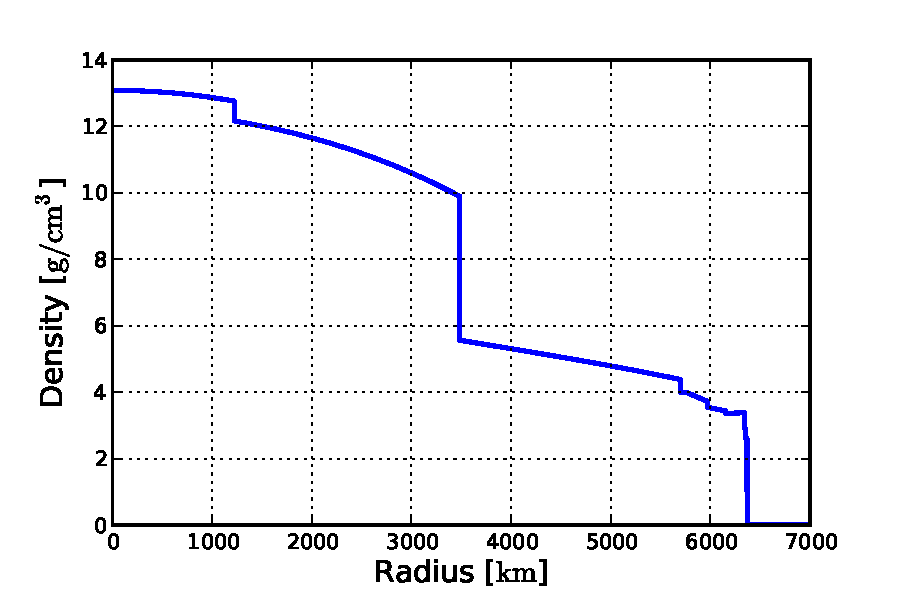
\includegraphics[width=0.7\textwidth]{PREM}
 \caption{The PREM Earth density profile \cite{PREM}.}
 \label{fig:PREM}
\end{figure}

Another feature of neutrino oscillations in matter are parametric enhancements. 
In contrast to MSW resonances, they depend on the shape of the matter potential 
rather than its actual value.

As shown in Fig.~\ref{fig:PREM}, the density profile and hence the matter 
potential of the Earth is characterised by to major regions: the core in the 
centre, with a radius of $\approx 3500$\,km, surrounded by the 
mantle\footnote{The Earth crust has a thickness of only a few tens of km and 
can thus be neglected.}. Within these regions, the density is rather constant 
at $\approx 11$\,g/cm$^3$ and $\approx 5$\,g/cm$^3$, respectively, while at the 
transition between the regions the density changes by almost a factor of two 
quasi instantaneously. 

\begin{figure}[th]
 \centering
 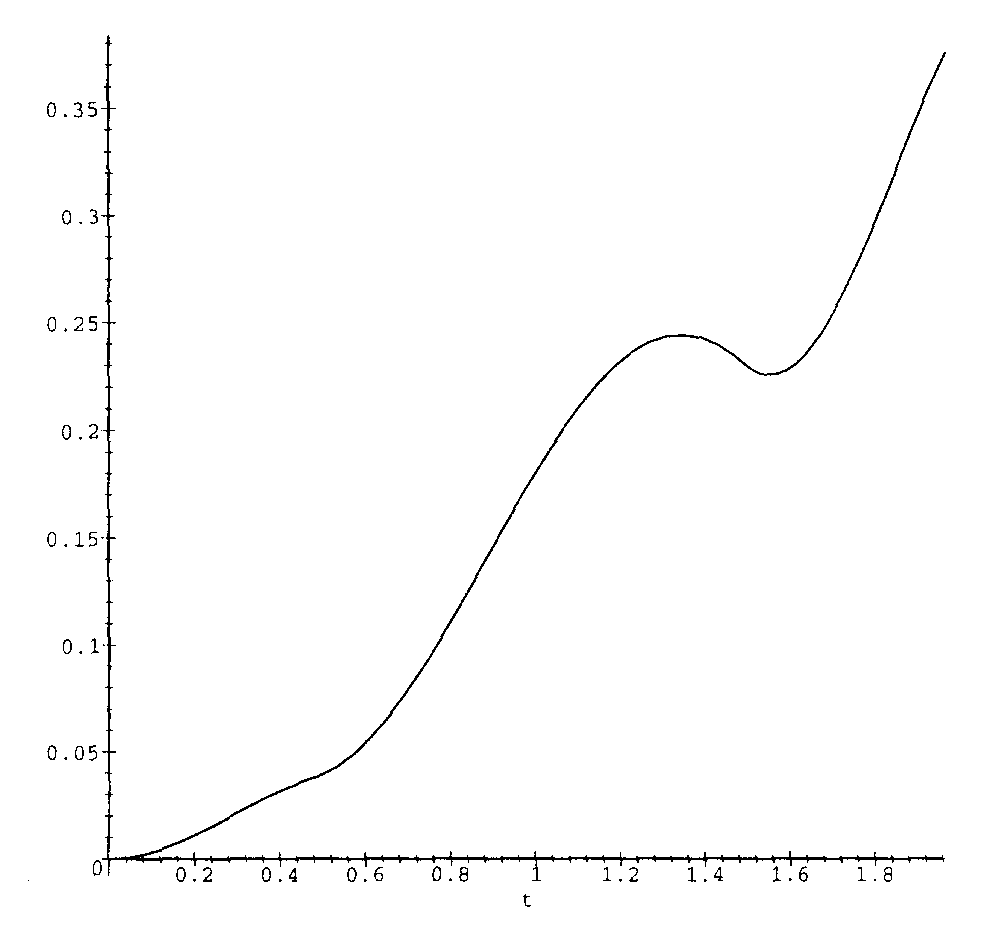
\includegraphics[width=0.5\textwidth]{ParamRes}
 \caption[\nue disappearance probability (qualitatively) as a
  function  of the distance $t$ (measured in units of the Earth's radius) along
  the  neutrino trajectory. Figure adopted from \cite{ParamRes2}.]
  {\nue disappearance probability (qualitatively\footnotemark) as a  function
  of the distance $t$ (measured in units of the Earth's radius) along  the
  neutrino trajectory. Figure adopted from \cite{ParamRes2}.}
 \label{fig:ParamRes}
\end{figure}

Thus for atmospheric neutrinos crossing the Earth, the matter potential can be 
approximated by a so-called ``castle-wall'' profile with good precision: First 
the neutrinos will experience a constant potential $A_\mathrm{CC}^m$ for a 
distance $l_m$ while passing through the mantle, with $A_\mathrm{CC}^m$ given 
by (\ref{eqn:mat_pot}) inserting the mean electron density in the mantle. 
Thereafter, they traverse the core, represented by another constant potential 
$A_\mathrm{CC}^c$ with a width of $l_c$, followed by a second crossing of the 
mantle that is symmetric to the first one.

\footnotetext{As \cite{ParamRes2} has been published already in 1999, the
values assumed for the mixing parameters do not coincide with the current best
fits. The effect in general, however, is the same for more up-to-date values.}

The principal resonance occurs if both $l_m$ and $l_c$ are close to half the
oscillation length (\ref{eqn:osc_length}) for the effective mass splittings 
(\ref{eqn:matter_massdiff}) in the respective regions \cite{ParamRes,
ParamRes2}:
\begin{equation}
 \frac{l_m}{L^\mathrm{osc}_m} = \frac{l_c}{L^\mathrm{osc}_c} = \frac{1}{2}
\end{equation}
This can be achieved by choosing an appropriate zenith angle at
which the neutrinos pass through the Earth.

Although the actual calculation of the oscillation probability is rather
involved \cite{ParamRes2}, the principal effect can be understood qualitatively:
The transition probability is close to its maximum when the neutrinos cross the
border between mantle and core, as shown in Fig.~\ref{fig:ParamRes}.
At this point, the matter potential changes, thus the neutrino state has to be
projected into the flavour base in which interactions have to be evaluated.
This re-sets the effective propagation length the neutrinos have travelled to
zero, such that the oscillation probability does not decrease after reaching
its maximum in the first region. Instead, the oscillation is ``restarted'' and
the oscillation probability in the second region is added to the one at the
transition between the regions. The same happens at the second region
transition, back from the core to the mantle, hence the final oscillation
probability after passing through the Earth is vastly enhanced \wrt the
non-resonance case.

These parametric enhancements depend on the neutrino mass hierarchy in the same
way as the MSW resonance, so they will also contribute to the NMH signature to
observe with PINGU, yet on a smaller scale than said resonance as it will be
shown in Sec.~\ref{sec:PINGUosc}.

\section{Oscillation Experiments}
\label{sec:OscExp}

Over the course of the last decades, a variety of experiments targeting most of
the possible neutrino sources listed in Sec.~\ref{sec:NuSources} have observed
oscillations. Consequently, measured values for all of the mixing angles and
mass splittings have been published, leading to a fairly consistent global
picture \cite{Fogli,GonzalezGarcia}. The most prominent of these experiments 
will be presented in this section, followed by an overview of the current 
best-fit values of the oscillation parameters.


\subsection{Solar Neutrinos}

As mentioned previously, already in the first detection of solar electron
neutrinos from the decay of $^8$B in the Homestake experiment in the 1960s
\cite{DaviesNuOsc}, neutrino oscillations had been observed in the form of a
lower than expected event rate. Although oscillations had been considered as the
cause for the deficit \cite{HomestakeLongterm}, a measurement of the 
all-flavour solar
neutrino flux was needed to exclude possible errors in the flux calculation.
This was provided later by the Kamiokande experiment \cite{SuperKsolar}, however
not in sufficient precision.

The required precision was finally reached by the SNO experiment, thereby making
the first definite observation of solar electron neutrinos oscillating to other
flavours \cite{SNOsolar, SNOosc}. In a two-flavour approximation, values for
\dm{21} and \thet{12} could be published as well \cite{SNOparams}.

\subsection{Atmospheric Neutrinos}

The very first conclusive observation of neutrino oscillations was the
disappearance of atmospheric muon neutrinos at energies around 1\,GeV, reported
by the Super-Kamiokande collaboration in 1998 \cite{SuperKosc}. This detection
was facilitated by a large value of the relevant mixing angle \thet{23}, which
is close to the maximum mixing value of $\pi/4$. Over the course of the last
years, more data have been added to this analysis, improving its precision on 
the measured parameters \thet{23} and $\dm{}=(\dm{31}+\dm{32})/2$.

Additionally, a similar measurement has been done with the IceCube DeepCore
neutrino telescope at energies of several tens of GeV \cite{DCosc}. Reaching a
comparable accuracy after a much shorter livetime, this result demonstrated that
a precision oscillation measurement is possible with a detector using a natural
target at which experimenters have much less control than over an artificial 
one.
DeepCore's success has paved the way for PINGU \cite{LoI}, which will map
atmospheric oscillations in the full three flavour picture with unprecedented
accuracy\footnote{With ORCA \cite{ORCA}, a very similar experiment has been
proposed that is supposed to do the same measurement, only using sea water
as detection medium instead of ice.}.

\subsection{Neutrino Beams}

Experiments aiming at atmospheric neutrino oscillations have both the problem
and the benefit that they will observe events over a large energy spectrum that
come from all directions. Although it provides a large lever arm for fitting
oscillation parameters, this also means that there is a fairly large uncertainty
from event reconstruction.

A way to overcome that problem is to use a controllable neutrino source, such as
a neutrino beam from an accelerator pointing towards a dedicated detector. Then,
the total flux as well as the energy and arrival direction of the neutrinos is
known, and one can concentrate on determining the oscillation
parameters---especially the mass splittings, which depend strongly on a precise
knowledge of the neutrino energy. If the value of the mixing parameter one is
about to constrain is roughly known beforehand, one can even fine-tune the
accelerator settings to reach maximal precision.

Examples are the MINOS \cite{MINOSparams} and T2K \cite{T2Kparams} experiments,
both using a \numu beam from Fermilab or J-PARC, respectively, to measure
\dm{31} and \thet{23}---the same parameters accessible for atmospheric
oscillations, thus providing an uncorrelated measurement.

Another goal that can be achieved with neutrino beams due to their high and
well-known flux and clean flavour composition is the search for the appearance
of neutrinos that have oscillated to other flavours. This has been done in T2K,
where the appearance of \nue has been observed \cite{T2Kapp}, and also in
OPERA, an experiment dedicated to search for \nutau events appearing in a \numu
beam from CERN \cite{OPERAapp}.

\subsection{Reactor Neutrinos}
\label{sec:ReacNuOsc}

Finally another class of experiments uses the strong flux of \nuebar at low MeV
energies produced by commercial nuclear reactors to study neutrino
oscillations. Typically, they consist of one ``near'' detector as close to the
reactor core as possible to achieve a precise normalisation of the
un-oscillated neutrino flux, and one ``far'' detector in the first oscillation
minimum, usually at several kilometers distance.
The relevant mixing parameter in this regime is \thet{13}, the last one to be
measured. The first measurement of \thet{13} was published in 2012 by the Daya
Bay experiment \cite{DayaBay}, subsequently confirmed by RENO and Double Chooz
\cite{RENO, DoubleChooz}.

With reactor neutrinos, also the mass hierarchy is accessible. If a far detector
is placed at a distance of $\approx 50$\,km, the small difference between
\dm{31} and \dm{32} will cause a fastly oscillating interference pattern on top
of the principal oscillation probability, whose exact shape depends on the mass
hierarchy. This measurement employs a different effect than the hierarchy
determination in atmospheric oscillations, thereby providing a completely
independent confirmation with different systematic effects. Even if neither of
the two experiments achieves a conclusive significance on its own, the
combination of both can vastly enhance the results \cite{BlennowSchwetz}. This
will be shown for the combination of PINGU with JUNO\footnote{Initially named
Daya Bay II.} \cite{JUNO, JUNO2} in Sec.~\ref{sec:JUNO}.

\subsection{Current Status of Neutrino Mixing Parameters}
\label{sec:MixingParams}

Global fits to neutrino oscillation results from different experiments are
available from various authors and usually constantly updated once new results
are published. For this thesis, the best fit values and uncertainties from Fogli
et al.\ released in 2012 \cite{Fogli2012} are used, which include the results
on \thet{13} from Daya Bay and RENO that where published shortly before. There
are more recent analyses available (e.\,g.\ \cite{Capozzi2013,
GonzalezGarcia2014}), but the differences are small as no major results have
been released in the meantime.
% FIXME: Use GonzalezGarcia2014 for the calculation? Most recent and best
% convention for mass splitting

\begin{figure}
 \centering
 \includegraphics[width=0.5\textwidth]{NMH}
 \caption{Schematic depiction of the ordering of neutrino mass eigenstates in
    both normal and inverted mass hierarchy. The definition of \dm{} and $\delta
    m^2$ according to Fogli et al.\ \cite{Fogli2012} is indicated as well.}
 \label{fig:NMH}
\end{figure} 
Since one of the neutrino mass splittings has a much smaller value than the
others, the convention is to label the two mass eigenstates that are close to
each other as $m_1$ and $m_2$, with $m_1 < m_2$ since the sign of the small
splitting has been determined using solar neutrinos (cf.\ Sec.~\ref{sec:MSW}).
The third eigenstate $m_3$ is then separated from the first two, either
above---in the ``normal'' mass hierarchy (NH)---or below in the ``inverted''
hierarchy (IH). This is illustrated in Fig.~\ref{fig:NMH}.

Since only two of the neutrino mass splittings are independent, Fogli et al.\
choose to do their analysis in terms of one small and one large mass splitting:
\begin{eqnarray}
 \delta m^2 &\equiv& m_2^2 - m_1^2 = \dm{21} > 0 \\
 \dm{} &\equiv& m_3^2 - \left(m_2^2 + m_1^2\right)/2 = \frac{\dm{31}+\dm{32}}{2}
   = \dm{31} - \dm{21}/2 \quad
   \begin{cases}
    \quad > 0 &\mbox{for NH} \\ \quad < 0 &\mbox{for IH}
   \end{cases}
\end{eqnarray}
The values and $1\sigma$ ranges given in \cite{Fogli2012} for $\delta m^2$,
\dm{}, \sinsq{\thet{12}}, \sinsq{\thet{23}}. and \sinsq{\thet{13}} have to be
converted to \dm{21} and \dm{31} and the values of the mixing angles in degrees
in order to be processed by the oscillation code calculating the transition and
survival probabilities. These values, which will be used as the \emph{fiducial}
oscillation parameters, are listed in Tab.~\ref{tab:fiducial_osc}. The CP
violating phase $\delta_\mathrm{CP}$ is set to zero.

\begin{table}[bht]
\caption{Fiducial values of the oscillation parameters, according to Fogli et
al., used throughout this thesis.}
\label{tab:fiducial_osc}
\begin{center}
\begin{tabular}{lcc}
\toprule
Parameter & Best Fit & $1\sigma$ Range\\
\midrule
\dm{31} [$10^{-3}\si{eV}^2$] &
\begin{tabular}[c]{@{}c@{}} 2.46 (NH) \\ -2.38 (IH)\end{tabular} & 0.08 \\
\dm{21} [$10^{-5}\si{eV}^2$] & 7.54 & 0.24 \\
\thet{12} [$^\circ$]         & 33.6 & 1.1 \\
\thet{23} [$^\circ$]         & 38.6 & 1.3 \\
\thet{13} [$^\circ$]         & 8.93 & 0.47 \\
\bottomrule
\end{tabular}
\end{center}
\end{table}

As one can see, the main unknown is the sign of \dm{31}, which will be assessed
by PINGU. Another remaining question is the octant of \thet{23}, i.\,e.\
whether its value is below or above \ang{45}. This unresolved as of now since
most oscillation experiments cannot measure the angle
directly, but rather \sinsq{2\thet{23}}, which is symmetric about \ang{45}.
Yet PINGU has good sensitivity to the octant of \thet{23}, and in addition the
significance of its hierarchy measurement is enhanced if $\thet{23} >
\ang{45}$, as one will see in Sec.~\ref{sec:results_octant}.
\enlargethispage{\baselineskip}

\section{Mass Hierarchy Signature in PINGU}
\label{sec:PINGUosc}

In the previous sections, all ingredients needed to
understand the measurement of the neutrino mass hierarchy PINGU is supposed to
perform have been discussed. These are
\begin{itemize}
 \item the atmospheric flux of \nue, \numu, and their antiparticles
       (Sec.~\ref{sec:AtmNus});
 \item their probabilities to convert to another flavour via neutrino
       oscillations in matter, especially the occurrence of the MSW resonance
       and parametric enhancement
       (Sec.~\ref{sec:matter_osc});
 \item and the cross-sections and peculiarities for the interaction of different
       neutrino flavours with the target material (Sec.~\ref{sec:NuDetection}).
\end{itemize}

The atmospheric neutrino flux as a starting point, follows a steeply falling
power law spectrum with an index of $\gamma \approx -3.7$ in all flavours.
The normalisation for \numu is about twice the \nue normalisation, while
neutrinos and antineutrinos of the same flavour have about the same flux. This
flux has to be multiplied by the oscillation probabilities, which depend not
only on the neutrinos' energies, but also on the zenith angle at which they 
arrive, since this determines the distance travelled since their production in
the Earth's atmosphere as well as the amount of matter traversed on their way
through the Earth.

In Figs.~\ref{fig:nue_to_numu} and \ref{fig:numu_to_numu}, the oscillation
probabilities for \nue to \numu and \numu to \numu are shown as examples. They
have been calculated using the AtmoWeights package that was developed by the
IceCube collaboration \cite{AtmoWeights} using the ``Preliminary Reference Earth
Model'' (PREM) \cite{PREM} for the Earth's density profile, shown in
Fig.~\ref{fig:PREM}. It is easily recognisable that the oscillation
probabilities for $\nu_\alpha \to \nu_\beta$ are in principle equal to those for
$\bar\nu_\alpha \to \bar\nu_\beta$, apart from the MSW resonance, easy to spot
in the energy range from 2 to \SI{10}{\GeV} for zenith angles between
$\coszen \approx -0.9$ and $-0.4$, that appears in neutrinos for the normal and
in antineutrinos for the inverted mass hierarchy (see
Sec.~\ref{sec:matter_osc}).
In addition, parametric enhancements occur for neutrinos passing through the
Earth's core, corresponding to the steepest zenith angles values below $\coszen
\approx -0.9$. These change between neutrinos and antineutrinos in the same way
as the MSW resonance, yet the latter covers a larger \coszen range and hence is
responsible for most of the mass hierarchy asymmetry.

\begin{figure}[p]
 \centering
 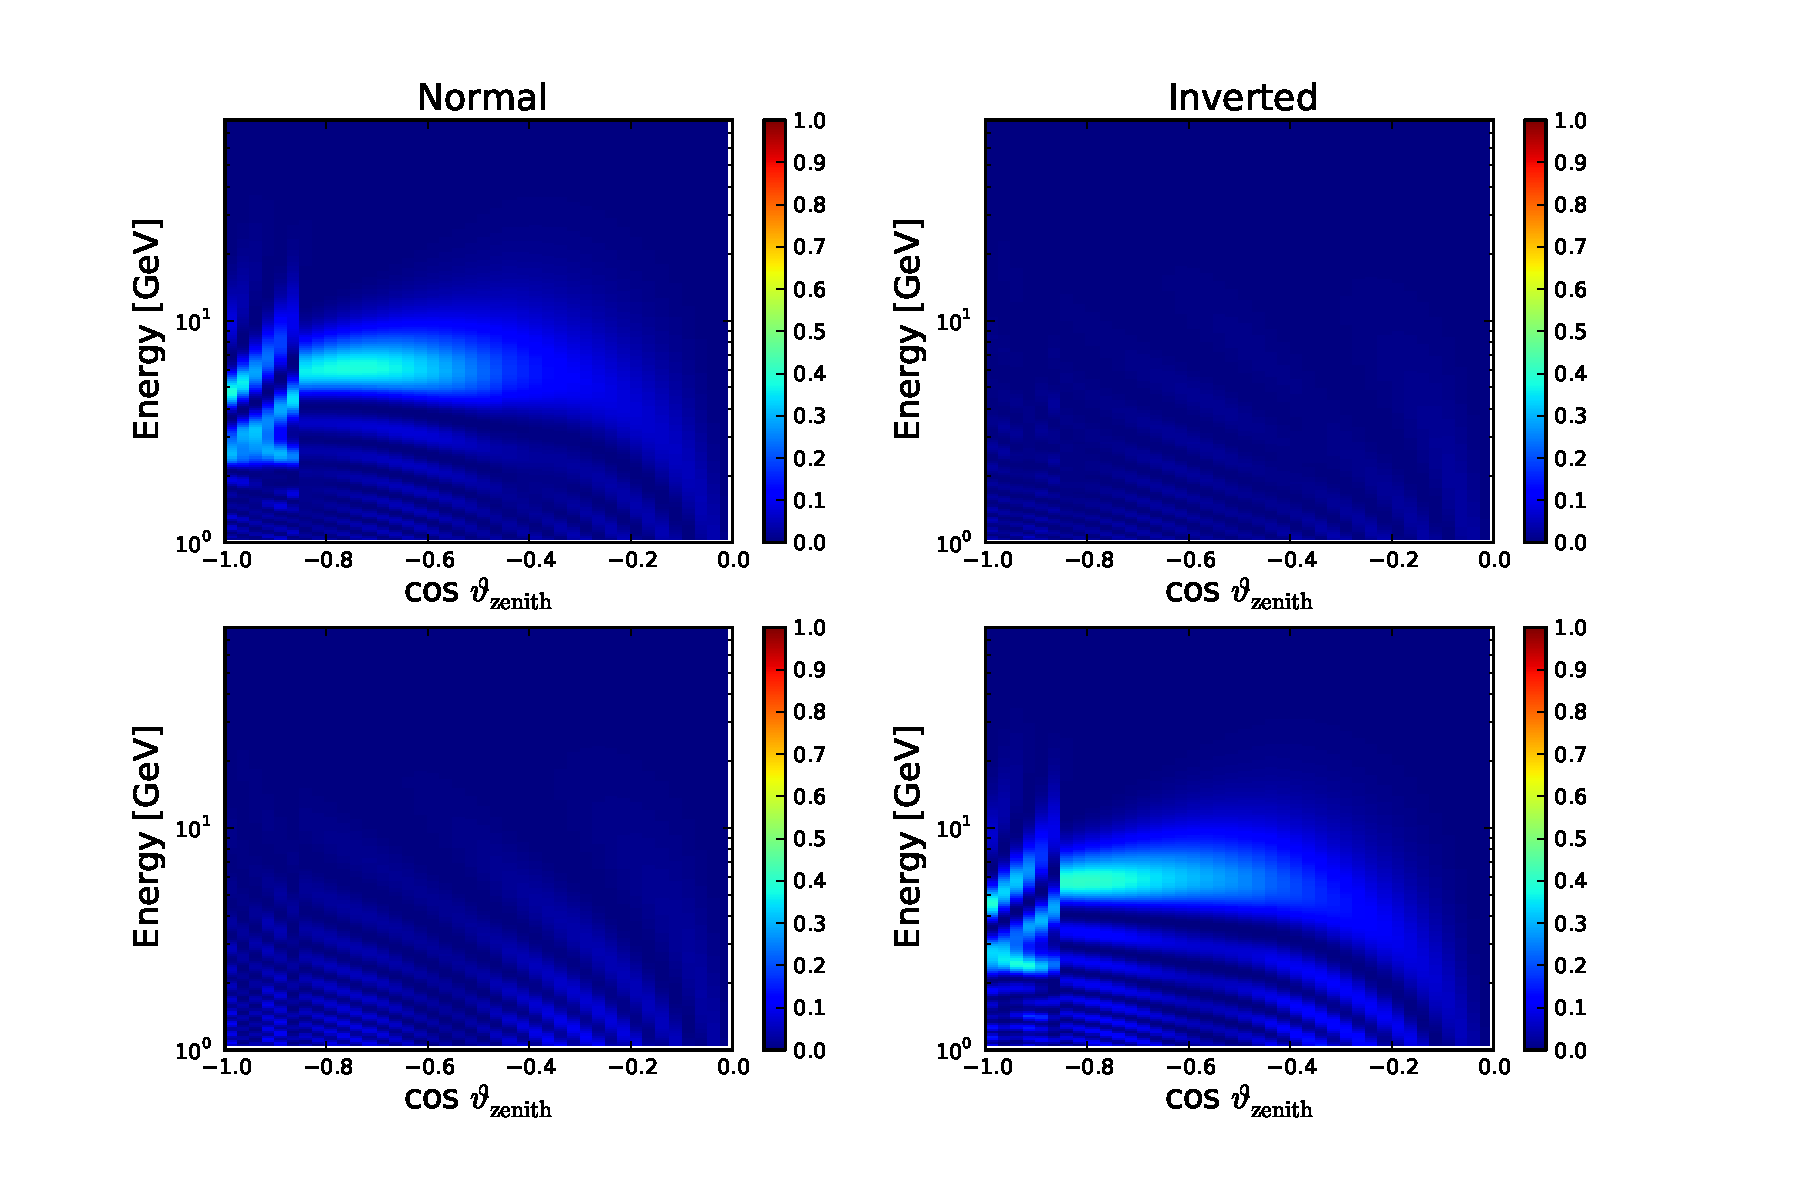
\includegraphics[width=0.95\textwidth]{osc_nue_to_numu}
 \caption{Oscillation probabilities for $\nue \to \numu$ (top) and $\nuebar \to
          \numubar$ (bottom) for normal and inverted hierarchy.}
 \label{fig:nue_to_numu}
\end{figure}
\begin{figure}[p]
 \centering
 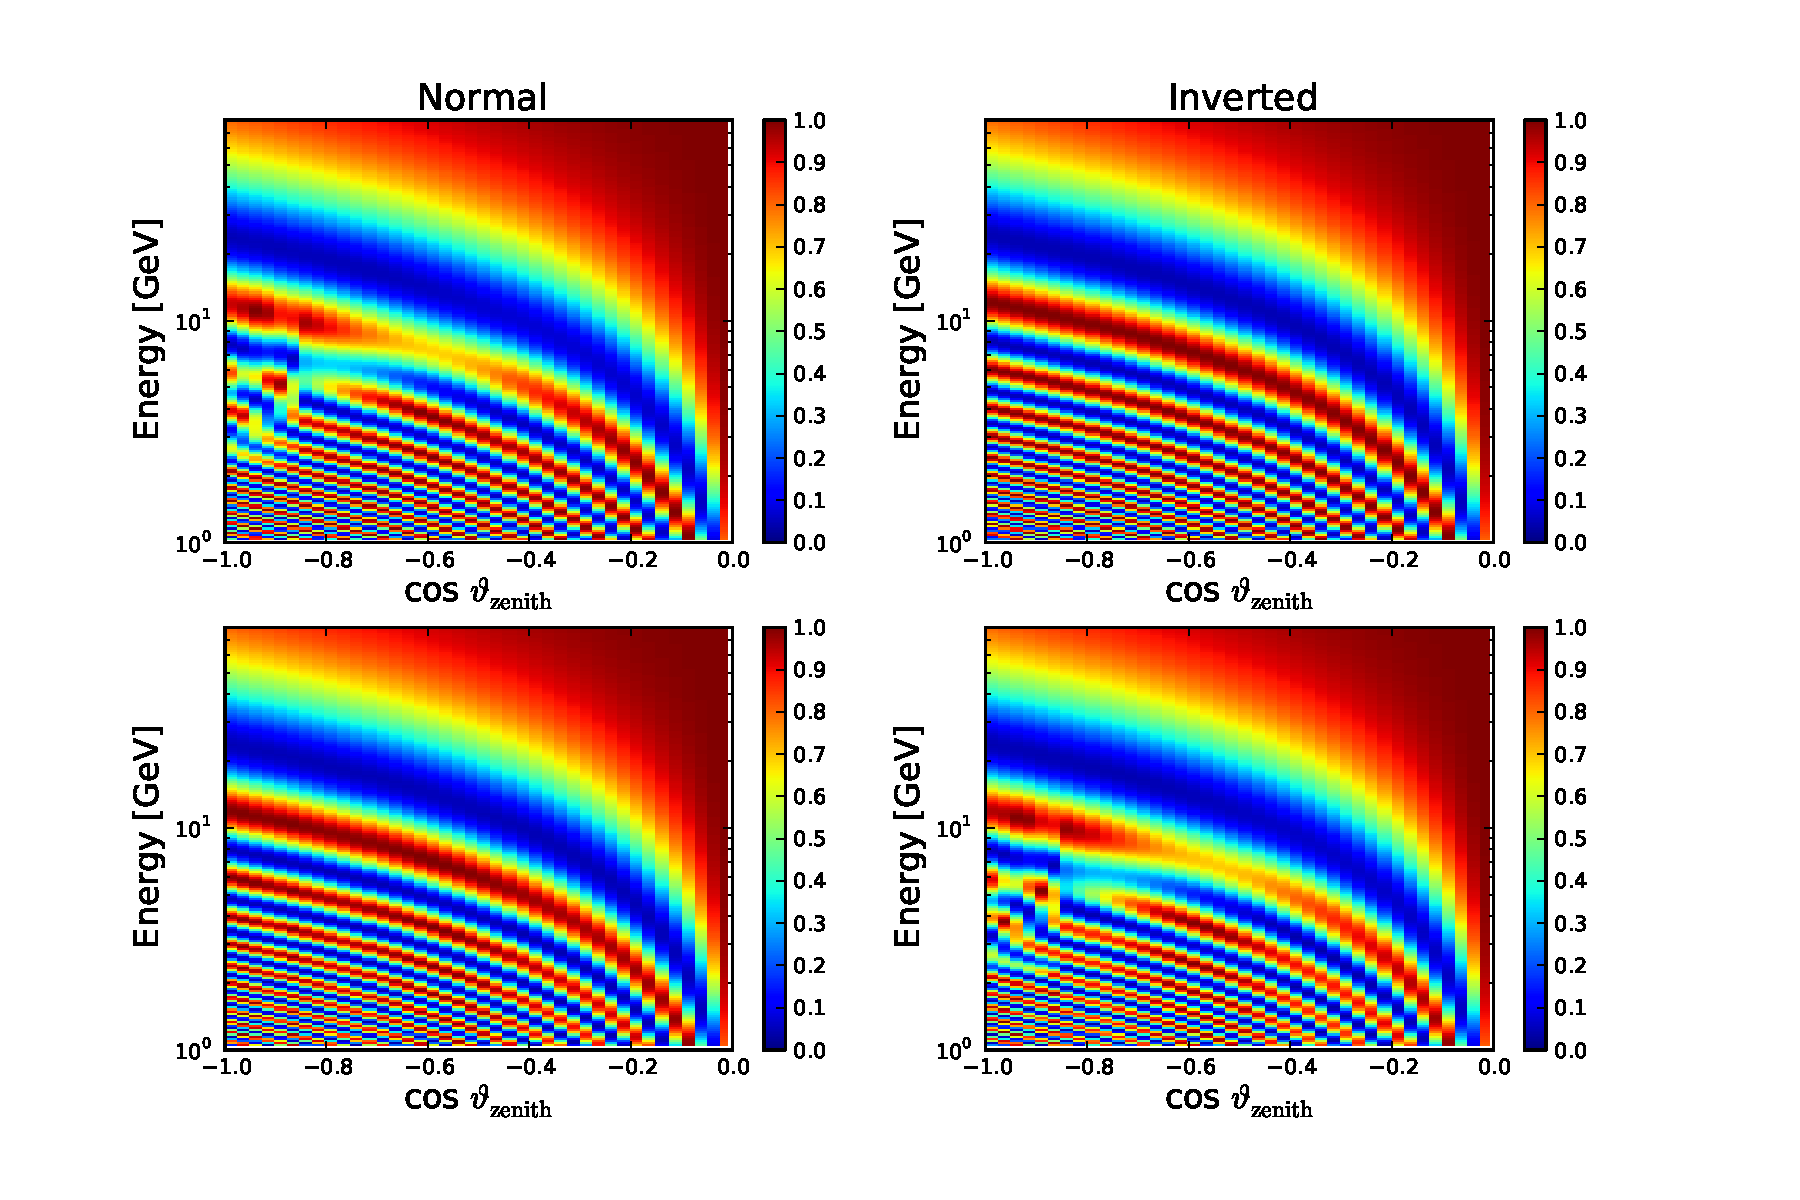
\includegraphics[width=0.95\textwidth]{osc_numu_to_numu}
 \caption{Oscillation probabilities for $\numu \to \numu$ (top) and $\numubar 
          \to \numubar$ (bottom) for normal and inverted hierarchy.}
 \label{fig:numu_to_numu}
\end{figure}

\enlargethispage{\baselineskip}
But since the fluxes of neutrinos and antineutrinos of the same flavour are 
essentially equal and PINGU cannot discriminate between them\footnote{The only
method to do this would be to identify the sign of the electrical charge of 
the lepton
produced in CC interactions. However it is unrealistic to generate the required
magnetic field in the antarctic glacier, where PINGU will be located (see
Secs.~\ref{sec:ICDC} and \ref{sec:PINGU}).}, the question is how the different
hierarchies can show up in the recorded data. Here the different cross-sections
for neutrinos and antineutrinos come into effect. As one can see from
Fig.~\ref{fig:NuXsec_GeV}, at the relevant energies just below \SI{10}{\GeV}
the cross section for antineutrino interactions with a hadronic target
material is about a factor of two lower than the one for neutrinos. Thus, the
MSW resonance will appear in the data in any case, but much more prominent if
the hierarchy is normal, as in this case roughly \sfrac{2}{3} of the
events---the neutrino-induced ones---are affected by it, while in the inverted
hierarchy case only the remaining third caused by antineutrinos is.

So the quantities of interest are the sum of neutrino and antineutrino events
for the different flavours at the energy and \coszen range where the MSW 
resonance is expected and how they differ assuming normal and inverted mass
hierarchy. To assess how significant the difference is in a given bin in the
($E$, \coszen) plane, a bin-wise \delchi similar to \cite{Akhmedov} can be
defined as
\begin{equation}
 \delchi = \frac{N_\mathrm{NH} - N_\mathrm{IH}}{\sqrt{N_\mathrm{NH}}} \quad,
\end{equation}
where $N_\mathrm{NH}$ and $N_\mathrm{IH}$ are the expected number of events in
the normal and inverted hierarchy case, respectively. Plots of the event rates
and their weighted difference \delchi are shown in
Figs.~\ref{fig:true_akhmedov_nue} to \ref{fig:true_akhmedov_nutau}. In this
calculation not the bare cross-sections, but rather the \emph{effective
areas} for the different flavours enter, which also include the detection 
threshold
and selection efficiency of the detector. This will be discussed in detail in
Sec.~\ref{sec:sim_input}.

Comparing the different flavours, one notes that the largest overall scale of 
the
\delchi values appears in the \numu channel, but the contiguous regions of
either positive or negative \delchi are rather small and alternate rapidly.
Since a realistic detector has a limited resolution in reconstructing individual
events, it will be challenging to resolve these fine structures in the data. In
the \nue channel, the features are less pronounced, but more extended than for
\numu, offering a more robust measurement.

\begin{figure}[p]
 \centering
 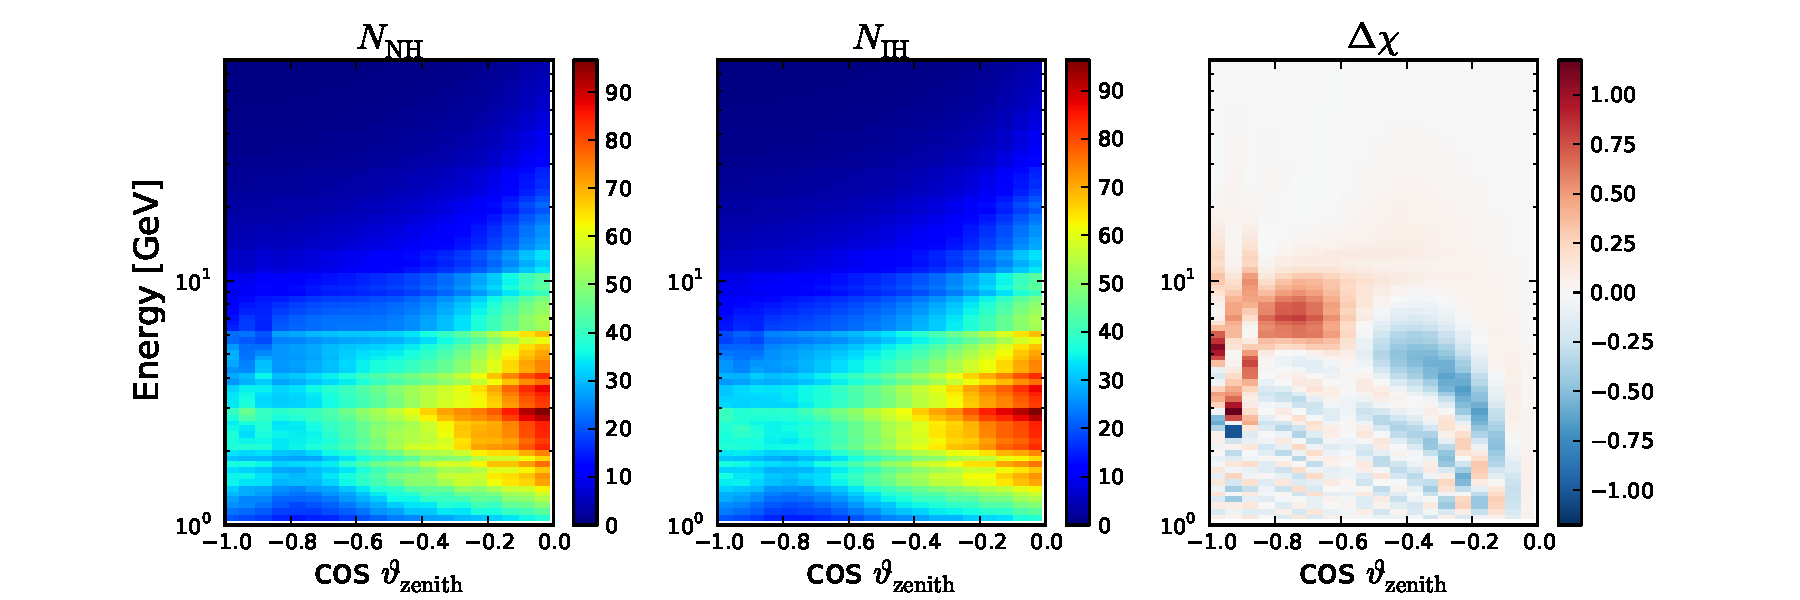
\includegraphics[width=\textwidth]{true_akhmedov_nue}
 \caption{Expected \nue + \nuebar CC event rates in PINGU (arbitrary units) for
    normal and inverted mass hierarchy and their weighted difference \delchi.}
 \label{fig:true_akhmedov_nue}
\end{figure}
\begin{figure}[p]
 \centering
 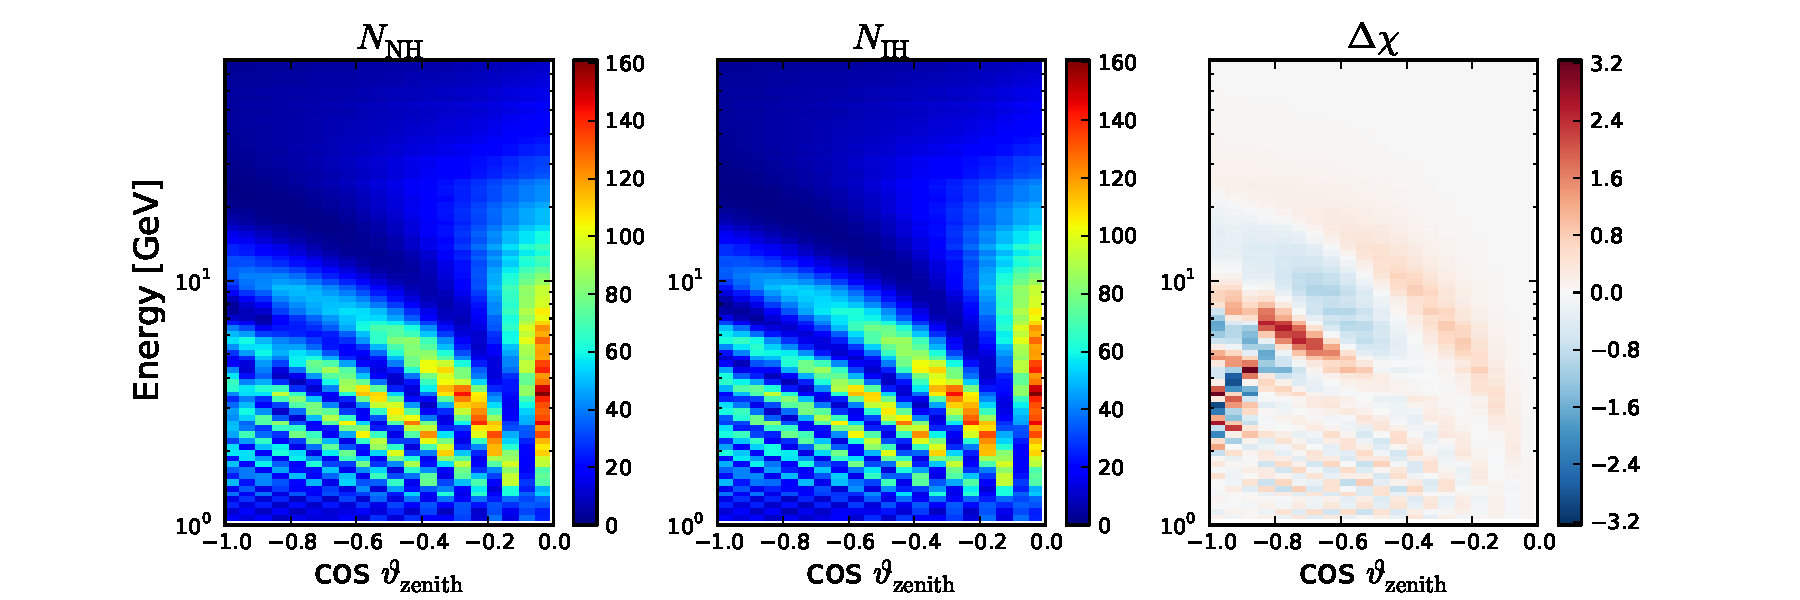
\includegraphics[width=\textwidth]{true_akhmedov_numu}
 \caption{Same as Fig.~\ref{fig:true_akhmedov_nue}, but for \numu + \numubar
    events}
 \label{fig:true_akhmedov_numu}
\end{figure}
\begin{figure}[p]
 \centering
 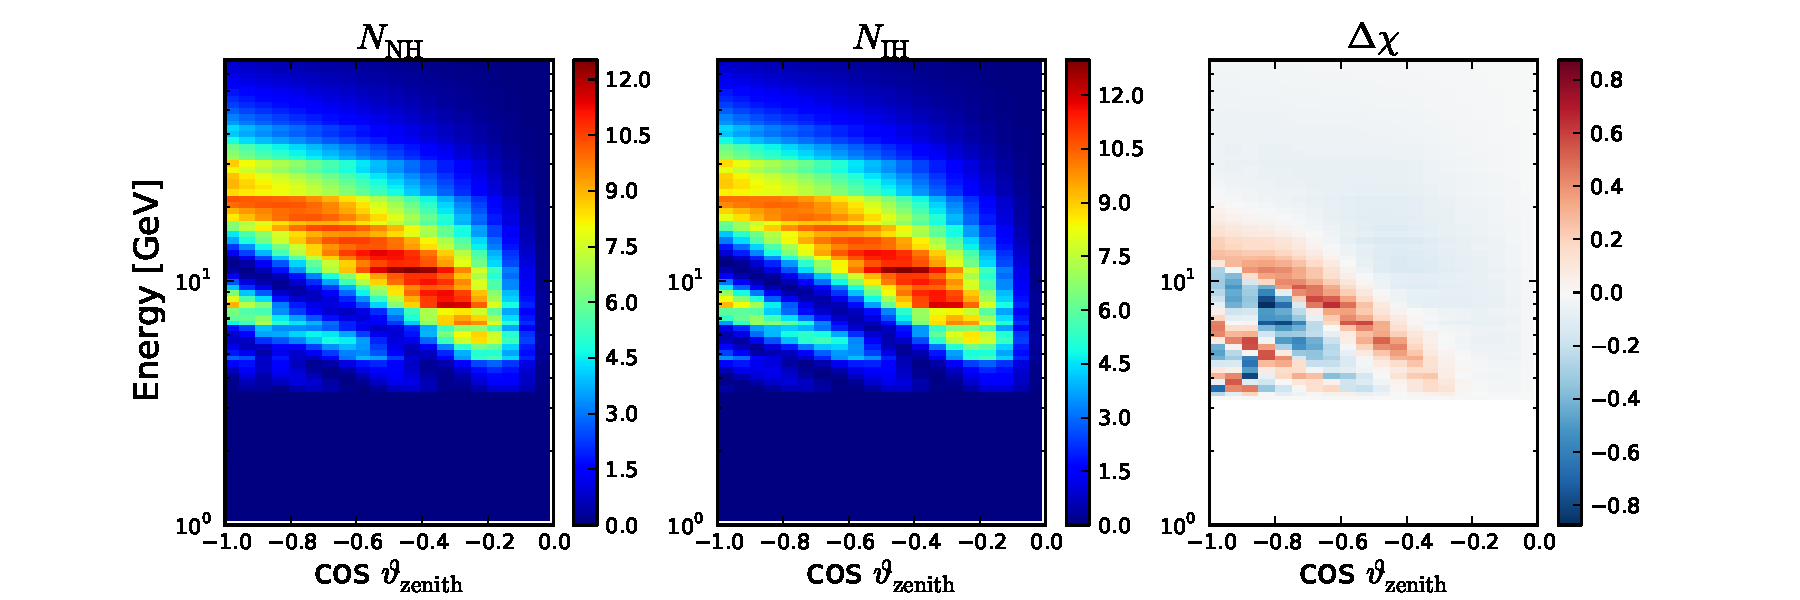
\includegraphics[width=\textwidth]{true_akhmedov_nutau}
 \caption{Same as Fig.~\ref{fig:true_akhmedov_nue}, but for \nutau + \nutaubar
    events}
 \label{fig:true_akhmedov_nutau}
\end{figure}


%==============================================================================
\chapter{Detector}
\label{sec:det}
%==============================================================================

In this chapter, a detailed description of the proposed PINGU neutrino
telescope and its predecessor IceCube will be given. We will start with
introducing the concept of ice or water based neutrino telescopes based on the
detection of Cherenkov radiation with IceCube/DeepCore as example, followed by
a characterisation of its upcoming PINGU upgrade.
Thereafter we will discuss how physics events will be selected and
reconstructed in an analysis targeting the determination of the neutrino mass
hierarchy, and finally how conceptually new hardware might improve the results.

%==============================================================================
\section{IceCube/DeepCore}
\label{sec:ICDC}
%==============================================================================

\subsection{Location}
\label{sec:IClocation}

As already mentioned (Sec.~\ref{sec:NuDetection}), the natural choice for
observing the low natural fluxes of high energy neutrinos are water-based
Cherenkov detectors. Although the basic requirement---a sufficiently large
amount of water or ice---seems not very difficult to meet, there are additional
constraints that have to be addressed as well:

\begin{description}
 \item[Size:] Depending on the energy range one is interested in, the size of
  the detector has to be adjusted accordingly. Since the atmospheric flux
  decreases rapidly with increasing energy, one needs larger detectors to study
  higher fluxes. Roughly from the GeV scale upwards, the required dimensions are
  so big (several hundred metres) that artificial structures like the
  underground caverns of Kamiokande and Super-Kamiokande \cite{SuperKosc} are
  not feasible any more and one has to look for suitable natural locations.
 \item[Transparency:] Since the detection of neutrinos is based on recording
  Cherenkov radiation, i.\,e.\ photons in the optical and near UV regime,
  obviously the chosen medium has to be transparent for these photons. Here ice
  has an advantage over fluid water as it has very low absorption down to
  wavelengths of 300\,nm and below \cite{IceProps}, while the fluid starts to
  absorb significantly below 400\,nm \cite{WaterAbs}.
 \item[Purity:] Usually the experiments try to reconstruct the neutrino events
  as accurately as possible. Therefore it is desirable to record a large number
  of unscattered photons and hence a very clear environment\footnote{There might
  be, however, situations where scattering is desired, e.\,g.\ when only the
  neutrino energy is of interest, then strong scattering keeps the photons
  inside the detector for a longer time and hence increases the total number
  of detected photons, thereby improving the energy resolution}.
 \item[Shielding:] In high energy neutrino experiments, muons from atmospheric
  showers created by cosmic radiation (cf.\ Sec.~\ref{sec:AtmNus}) are a
  background process whose rate is several orders of magnitude higher than the
  neutrino signal. In order to suppress those muons, detectors have to be
  placed deep underground so that there is a shielding with several hundred
  meters thickness, comparable to the range of $\mathcal{O}
  (100\,\mathrm{GeV})$ muons.
\end{description}

\begin{figure}[htp]
 \centering
 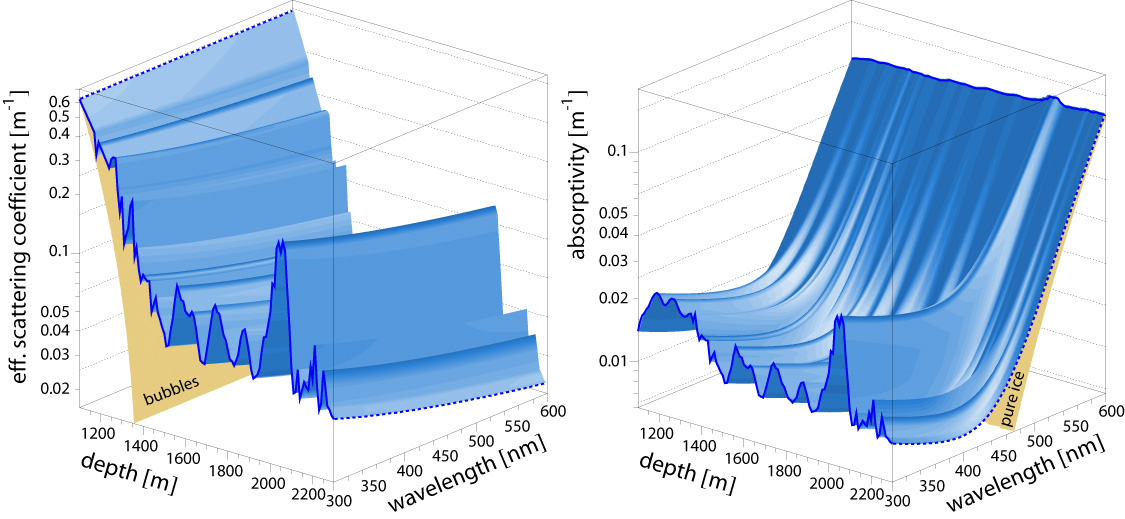
\includegraphics[width=\textwidth]{Icepaper_figure22_scatt-abs-length}
 \caption{Effective scattering and absorption of light in the polar ice. Plot 
  taken from \cite{IceProps}.}
 \label{fig:ice_scatt_abs}
\end{figure}

Choosing an environment optimising all these factors, the IceCube neutrino 
observatory has been constructed in the deep glacial ice at the geographical 
South Pole in Antarctica. The Antarctic glacier with its thickness of $\approx 
2500$\,m is a pristine environment of substantial size. In contrast to natural 
resources like lakes or the deep sea, it inherently provides a solid holding 
structure for the instrumentation, is free of lifeforms that might disturb or 
even destroy the detector, and has a much lower content of radioactive $^{40}$K 
than sea water. Especially at depths more than $\approx 2000$\,m below the 
surface, age and high pressure have facilitated the hydratisation of enclosed 
air bubbles, leaving an extremely clear ice with scattering and absorption 
lengths of several tens of metres even in the UV range, see 
Fig.~\ref{fig:ice_scatt_abs}. Instrumenting only the deepest ice below 1500\,m 
guarantees a sufficient shielding of atmospheric muons. 

The nearby Amundsen-Scott South Pole Station operated by the United States 
Antarctic Program provides the infrastructure needed for such a large scale 
experiment. This incorporates the supply of electrical power for the detector 
itself and the computing farm processing the raw data, satellite communications 
for transmitting science data, general technical support as well as 
accommodations for the visiting scientists.

\subsection{Detector Geometry}
\label{sec:ICgeometry}

A total of 86 strings, each instrumented with 60 Digital Optical Modules (DOMs, 
see Sec.~\ref{sec:ICDOM}), have been installed during IceCube's deployment phase 
from 2005 until December 18, 2010. A hot water drill was used to melt holes of 
60\,cm diameter into the ice, reaching down to 2450\,m, shortly above the 
underlying bedrock. Then the strings were lowered into the holes still filled 
with water which then refroze and firmly encloses the strings.

Eighty of those strings form the hexagonal main array with an inter-string 
distance of 125\,m, while the remaining six are placed at additional positions 
near the centre of the array, forming a dense sub-array with a string spacing 
of only 72\,m, lowering the threshold energy for neutrino detection from 
$\approx 100$\,GeV to $\approx 20$\,GeV. A top view of the string layout is 
shown in Fig.~\ref{fig:string_layout}.

\begin{figure}[htp]
 \centering
 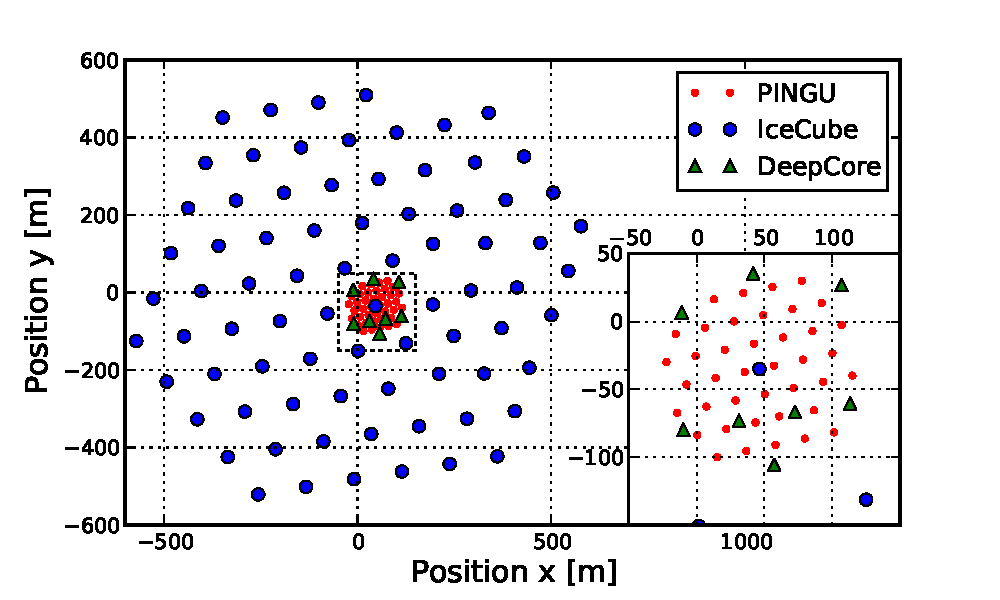
\includegraphics[width=\textwidth]{ic_dc_pingu_strings}
%  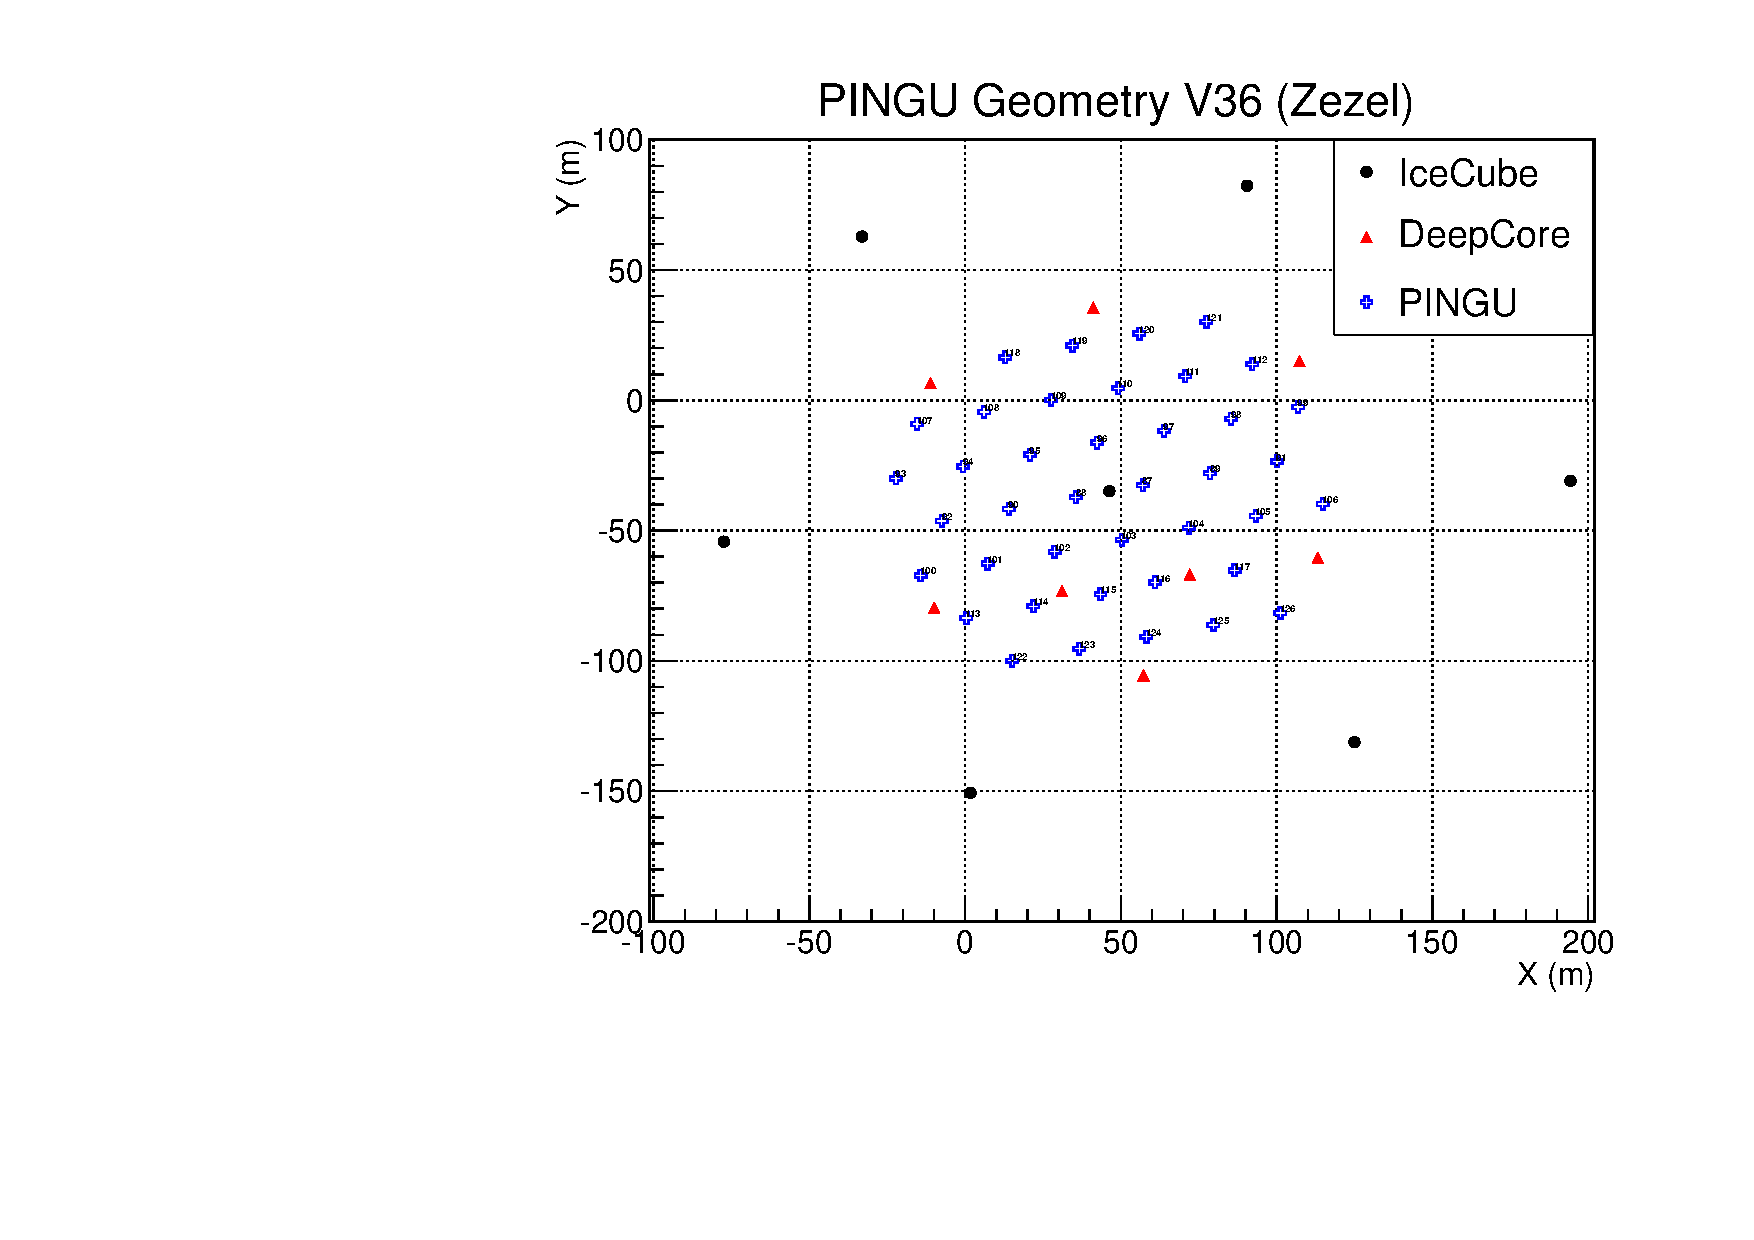
\includegraphics[width=0.7\textwidth]{pingu_V36_Zezel_40_s22_d3}
 \caption{Top view of the IceCube string layout, including the DeepCore and 
planned PINGU (geometry V36) sub-arrays.}
 \label{fig:string_layout}
\end{figure}

To the lowest 1000\,m of the main array strings, sixty DOMs each are attached, 
evenly spaced with a distance of 17\,m. In DeepCore, the vertical DOM spacing 
is only 7\,m below the dust layer found between 1950\,m and 2100\,m 
depth\footnote{The dust layer can be recognised easily in 
Fig.~\ref{fig:ice_scatt_abs} as the region of increased scattering and 
absorption.}, with a veto cap of ten DOMs with 10\,m spacing per DeepCore 
string above it \cite{I3Design,DCDesign}.


\subsection{Digital Optical Modules}
\label{sec:ICDOM}

\begin{figure}[htp]
 \centering
 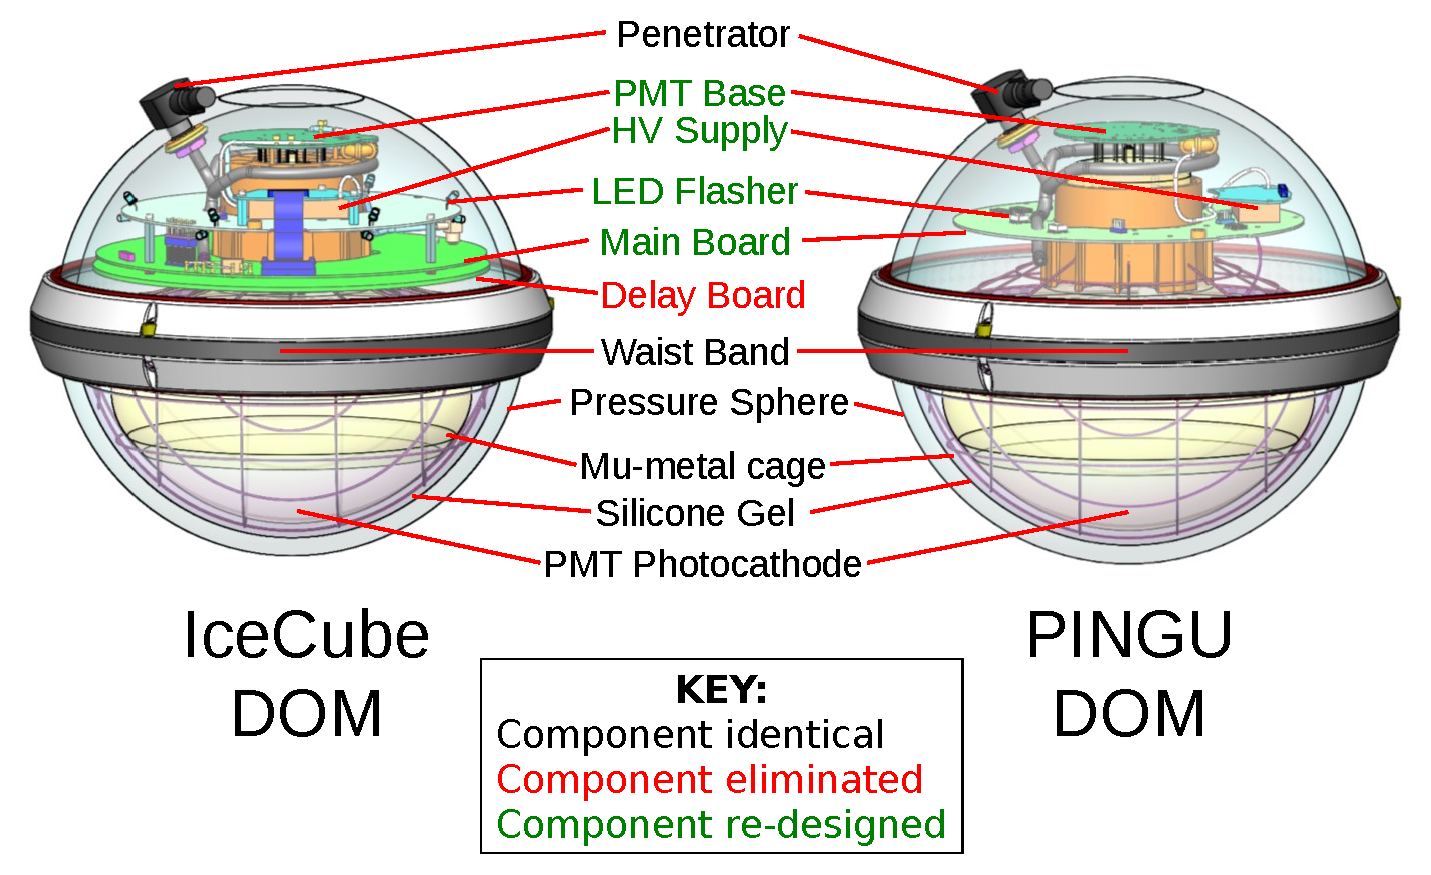
\includegraphics[width=0.7\textwidth]{I3DOM_PDOM_cropped}
 \caption{Comparing an IceCube/DeepCore DOM to the PDOM used in PINGU. Graphics 
taken from \cite{PDOM_Aachen}.}
 \label{fig:DOM}
\end{figure}

The 5160 Digital Optical Modules are the basic detection units of IceCube. They 
are attached to the string and connected to the main string cable during 
deployment and work autonomously except for the low voltage power supply. This 
modular design has the convenience that if one DOM fails to work and cannot be 
fixed as it is frozen in the deep ice, the others are not affected.

As shown in Figure \ref{fig:DOM}, the DOM is housed by a borosilicate glass 
sphere of 13\verb+"+ diameter and 0.5\verb+"+ thickness to withstand the 
pressure arising from the refreezing water in the drill holes. This glass sphere 
also contributes to the noise rate of about 540\,Hz per DOM as it contains 
isotopes of the uranium and thorium decay chains. The content of natural 
$^{40}\mathrm{K}$, that undergoes beta decay where the emitted $\beta$ particle
generates Cherenkov light, has been reduced in the glass.

The main component of the DOM is a 10\verb+"+ photomultiplier tube (Hamamatsu 
R7081-02 \cite{PMTpaper,PMTdata}). In DeepCore, an improved version of this PMT 
with a 35\,\% higher quantum efficiency was used \cite{DCDesign}. The PMT is 
oriented downwards as the main focus of IceCube is on extraterrestrial neutrinos 
from the northern hemisphere that have travelled through the Earth and hence 
arrive at the South Pole from below. The coupling to the glass sphere is 
provided by an optical gel which also provides protection and fixation to the 
PMT, while a surrounding Mu-metal grid guarantees the shielding of external 
magnetic fields.

The upper half of the DOM is filled with an high voltage divider that locally 
transforms the 96\,V voltage that is provided by the string main cable into the 
high voltage of 1.3--1.5\,kV that is needed to fuse the PMT, thus making it 
independent from possible voltage fluctuations of the pole station's power 
supply. Around the HV divider, the circular flasher board and DOM mainboard are 
mounted. The flasher board is populated with LEDs that can be used to produce a 
standardised signal for calibration. On the mainboard the electronics are 
located that are needed to read out the PMT signal and digitise the recorded 
data in situ, after which they are sent to the surface.



%==============================================================================
\section{PINGU}
\label{sec:PINGU}
%==============================================================================

PINGU, the Precision IceCube Next Generation Upgrade, is planned as a further 
infill to the IceCube/DeepCore array, lowering the energy threshold to few GeV 
\cite{LoI}. The current baseline geometry, V36, consists of forty additional 
strings with 96 PINGU-DOMs (PDOMs, see below) each. In this layout, shown in
Figs.~\ref{fig:string_layout} and \ref{fig:string_layout}, the string spacing is
22\,m while the PDOMs are located the lowest 300\,m of IceCube with a vertical
distance of 3\,m. In this depth, the same as the main part of DeepCore, the ice
has the best optical properties.

\begin{figure}[htp]
 \centering
 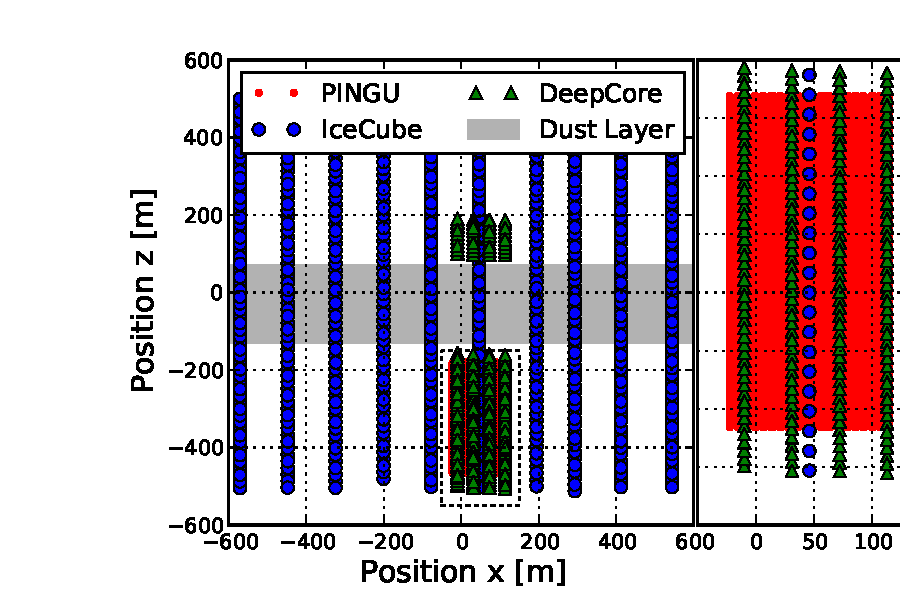
\includegraphics[width=0.8\textwidth]{ic_dc_pingu_sideview}
%  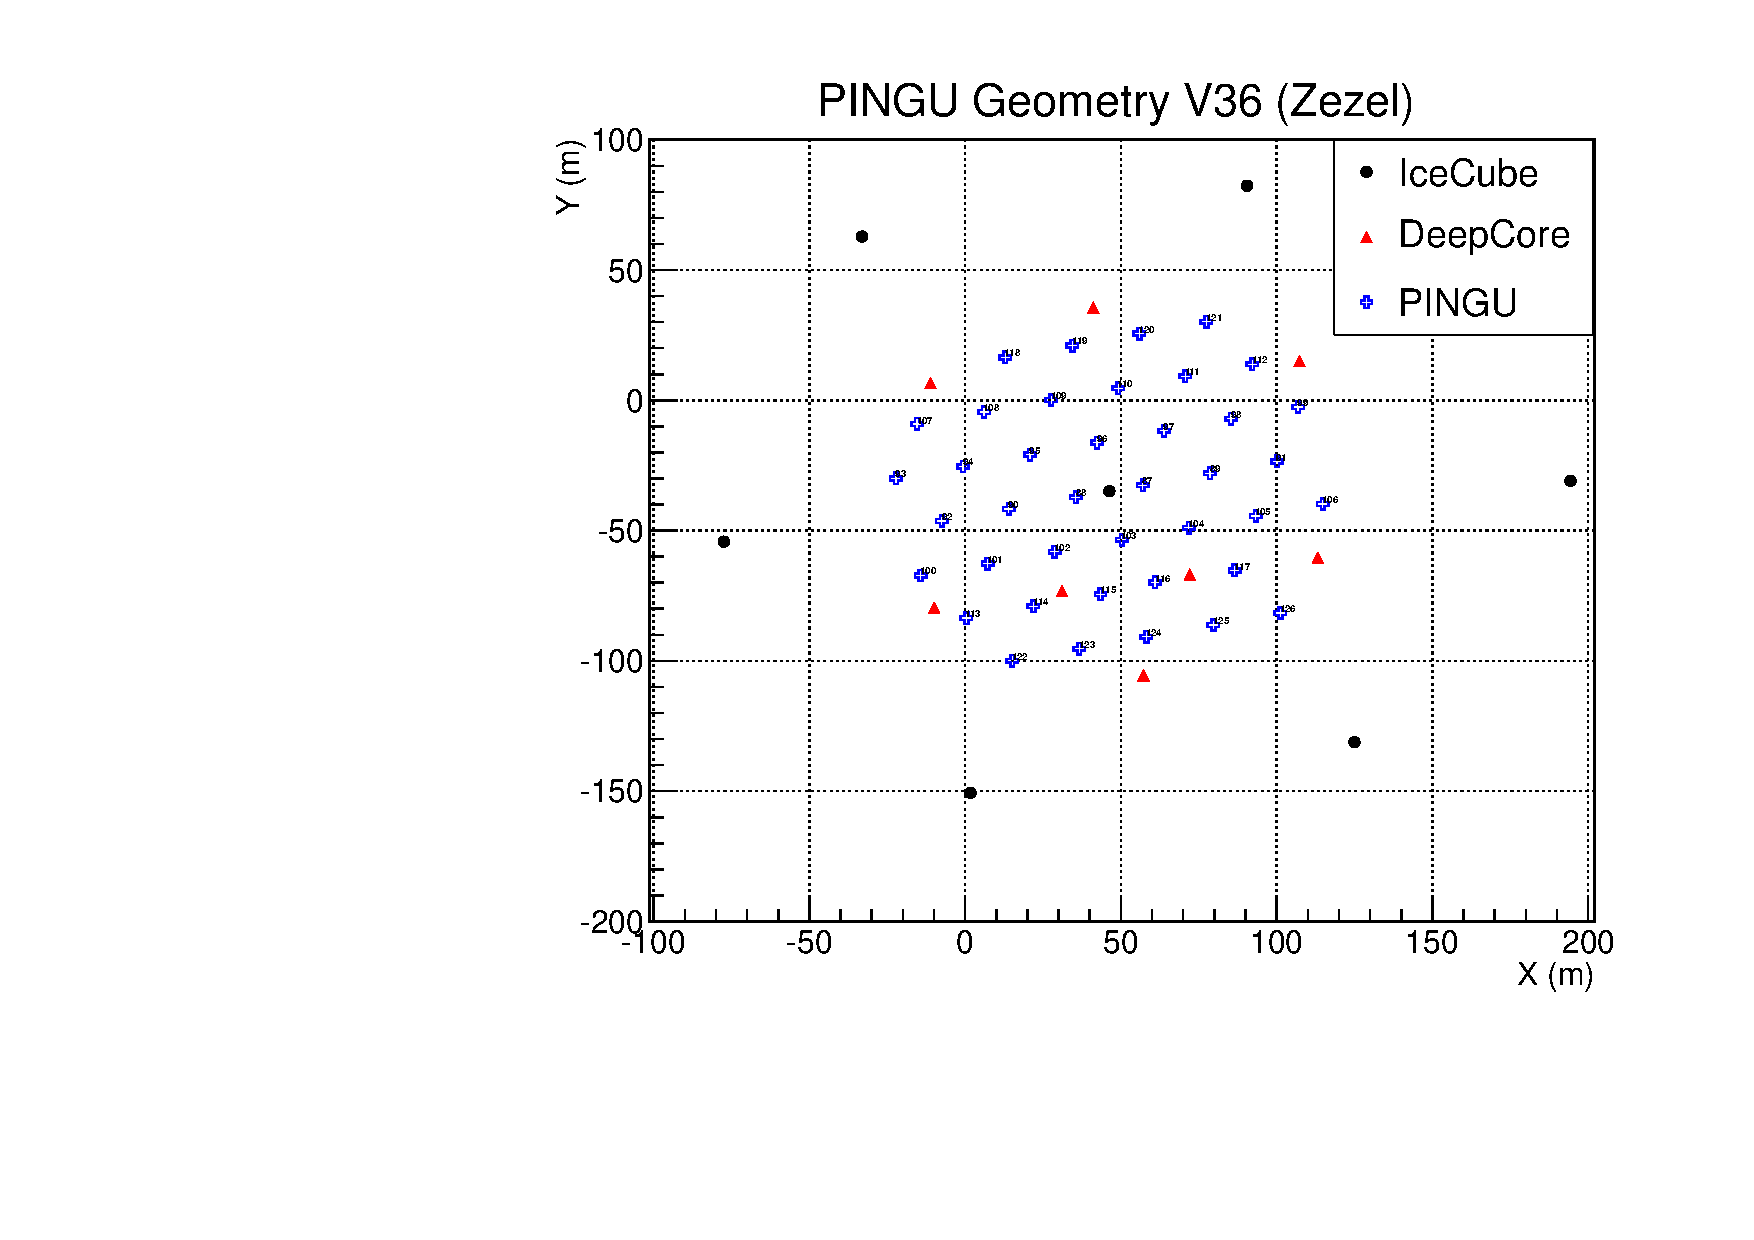
\includegraphics[width=0.7\textwidth]{pingu_V36_Zezel_40_s22_d3}
 \caption{Side view of the IceCube string layout, including the DeepCore and
  planned PINGU (geometry V36) sub-arrays. The approximate position of the dust
  layer is shown for reference.}
 \label{fig:string_layout_side}
\end{figure}

This detector geometry has been optimised to yield a maximum sensitivity for 
the neutrino mass hierarchy. It will be used for all studies described in 
Chapter~\ref{sec:ana} unless explicitly stated otherwise.

In terms of hardware and software infrastructure, many things can be adopted 
from IceCube, redesigning parts where a potential for improvement or 
simplification has been discovered. Several components of the electronics part
of the module, like the main board, the PMT base, and the high voltage supply,
have been redesigned or replaced by more recent versions. In particular the PMTs
will all be the high quantum efficiency models already installed in DeepCore.
A delay board has become obsolete with the more recent signal digitisers and
will not be part of the PINGU DOMs. Additional components, such as cameras to
monitor the freeze-in process, are in discussion.

Although the bulk of PDOMs are an improved version of the technology that has 
proven to work reliably, prototypes of novel optical modules will be deployed 
with PINGU as well. As those might be the baseline technology of future 
neutrino telescopes, they have to be tested under realistic conditions before 
they can be considered for large-scale use. Two options for these 
next-generation optical modules are described in Sec.~\ref{sec:Gen2DOM}, 
studies showing how they will impact the NMH determination are presented in 
Sec.~\ref{sec:om_effects}.

Another thing to be improved upon in PINGU is the so-called ``hole ice''. In 
IceCube it was observed that the refrozen ice directly around the strings that 
had been molten during deployment contains lots of small air bubbles. These 
inclusions lead to a dramatically reduced scattering length around the DOMs,
significantly deteriorating the quality of event reconstruction that strongly
profits from a large number of direct (i.\,e.\ unscattered) photons being
recorded. In order to reduce the impact of the hole ice, the molten water will
be degassed as a part of the drilling process for PINGU, thus reducing its air
content and hence the number of air bubbles remaining after refreezing.

%==============================================================================
\section{Event Reconstruction}
\label{sec:EvtReco}
%==============================================================================

To identify the features in the distribution of neutrino events recorded by
PINGU that are imprinted by the neutrino mass hierarchy, it is crucial to
reconstruct the events as exactly as possible. Although the interesting neutrino
properties are only its energy and the zenith angle of its arrival
direction\footnote{Which determines the length of propagation since the
creation in the Earth's atmosphere and the matter potential passed on the way.}
as those are determining the oscillation probability, an actual neutrino
interaction event in PINGU has far more properties that need to be
reconstructed as well. These are:
\begin{itemize}
 \item The position of the interaction vertex in both space and time, giving
  rise to four variables in total ($x,\,y,\,z,\,t$).
 \item The energy of the hadronic cascade caused by the fragmented target
  nucleus, $E_\mathrm{cscd}$.
 \item The direction of the hadronic cascade, described by its zenith and
  azimuth angles ($\theta,\,\phi$)
 \item The energy $E_\mu$ of the outgoing muon (if present), which can be
  replaced by its length $l$ since muons can be
  considered as minimum ionising particles (see Sec.~\ref{sec:NuDetection}).
 \item The direction of the muon, represented by zenith and azimuth angles
  ($\theta_\mu,\,\phi_\mu$) as well.
\end{itemize}
This amounts to a total of ten variables (seven if no muon is created in the
interaction) whose values have to be found in the reconstruction process. The
neutrino energy is then given by the sum of cascade and muon energy, and its
direction has to be calculated from their momenta using the conservation of the
total momentum. 


% \subsection{Low-Level Reconstruction}
% \label{sec:reco_lowlevel}
% TODO: write about it?

\subsection{CLast}
\label{sec:reco_clast}

The start of the reconstruction chain is CLast \cite{CLast}, a first-guess
algorithm for cascade, i.\,e.\ point-like events. With $vec{r}_i$ being the
positions of the DOMs that have registered charges $a_i$ at times $t_i$ in the
event, first the event vertex is determined a the centre of gravity (COG) of the
hit DOMs:
\begin{equation}
 \vec{x} = \sum_i a_i \vec{r}_i
\end{equation}

Following that, the time $t$ of the vertex is calculated. For this, the residual
time is defined as
\begin{equation}
 \tau_i(t) = t_i - \left( t + d_i/c_\mathrm{ice} \right) \quad,
\end{equation}
where $d_i = | \vec{x} - \vec{r}_i |$ and $c_\mathrm{ice} = c/n_\mathrm{ice}$ is
the speed of light in ice. After that, a direct hit is defined as a DOM hit
with $0 < \tau_i < t_w$, with a trigger window of $t_w = 200$\,ns. Now for each
DOM, a test vertex time is chosen to be $t_i - d_i/c_\mathrm{ice}$ and the
number of direct hits on all other DOMs is calculated. From all those test
vertex times, the earliest one resulting in more than four direct hits on other
DOMs is chosen as the vertex time $t$.

After the vertex position has been established, the cascade direction is
determined from the ``tensor of inertia'' of the hit pattern. In a reference
frame centred at the COG, $\vec{r}_i' = \vec{r} - \vec{x}$, this is calculated
analogue to the quantity in classical mechanics with the mass replaced by the
DOM charge:
\begin{equation}
 I^{k,l} = \sum_i a_i \left(\delta^{kl} \vec{r}_i'^2 - r_i'^k r_i'^l\right)
\end{equation}
The cascade direction is then given by the eigenvector corresponding to the
smallest eigenvalue of the tensor of inertia, which points along the strongest
elongation of the hit pattern.

Finally, a first estimate for the cascade energy is calculated using an
empirical polynomial fit \cite{Processing} to the number of hit DOMs in the
event, $N_\mathrm{Ch}$:
\begin{equation}
 \log_{10}\left(E_\mathrm{cscd} [\mathrm{GeV}]\right) =
  -3.3 + x\,(\,9.2 + x\,(\,-9.7 + x\,(\,5.3 + x\,(\,-1.4 + x\cdot 0.134))))
\end{equation}
with $x = \log_{10}(N_\mathrm{Ch})$.

\subsection{Photonics}
\label{sec:reco_photonics}

The Photonics software \cite{Photonics} is a tool widely used in IceCube to get
a fast description of the propagation of Cherenkov photons in the ice. Its main
functionality is to return the expected number of registered photons
$B(\vec{r}, \vec{x}, t, \theta, \phi)$ for any combination of source
$(\vec{x}, t, \theta, \phi)$ and sensor position $\vec{r}$.

Since photon propagation needs extensive computing, $B$ cannot be directly
simulated for each request. The number is retrieved from a table look-up
instead. The respective tables have to be generated in advance by simulating a
large number of sources in all possible depths---since the optical properties
of the Antarctic ice sheet depend strongly on the vertical position, see
Fig.~\ref{fig:ice_scatt_abs}---and all possible zenith angles, using data on the
ice properties that have been retrieved from onboard LED flasher signals
recorded by the IceCube DOMs \cite{Dima}. The resulting photon density
distribution is then stored in six-dimensional tables, the relevant quantities
being three spatial dimensions, the relative time between emission and
detection, the emission angle at the source, and the angle of incidence on the
detector since the DOMs have a zenith dependent detection efficiency, as clearly
visible from their layout (Fig.~\ref{fig:DOM}).

Finally these tables are fitted with multidimensional spline functions, which
leads to more smooth results and significantly reduces the amount of data that
has to be stored \cite{Dima}. This is an important issue, since one of those
six-dimensional tables has to be loaded into the CPU memory for every source
depth, orientation, and type (point-like and track-like, as these have
different light output distributions).

\subsection{Monopod}
\label{sec:reco_monopod}

The Monopod algorithm is an likelihood reconstruction for cascade-like events
using detailed photon timing information. It is the single source case of the
more general Millipede algorithm \cite{Millipede} that is used for high-energy
track reconstruction, where it segments an extended track into a series of
point-like energy depositions along the track.

Assuming a cascade-like energy deposition $E$ at the vertex position $\vec{x}$
and time $t$, pointing into the direction $(\theta, \phi)$, the expected number
of photons $B^\mathrm{cscd}_j(\vec{r}_i, \vec{x}, t, \theta, \phi)$ per unit
energy is retrieved from Photonics (see Sec.~\ref{sec:reco_photonics}) for every
DOM $i$ that registered photons in the event and for every time bin $j$. The
total number of expected photons is then
\begin{equation}
 \mu_{ij} = B^\mathrm{cscd}_j(\vec{r}_i, \vec{x}, t, \theta, \phi)
             \,E_\mathrm{cscd} + \nu_j  \quad, \label{eqn:cscd_hypo}
\end{equation}
where $\nu_j$ is the expectation of noise hits.

From this, a Poisson likelihood is constructed according to
\begin{equation}
 \mathcal{L} = \prod_i^\mathrm{\#\ hit\ DOMs} 
   \quad \prod_{j}^\mathrm{\#\ time\ bins}
   \frac{\mu_{ij}^{n_{ij}}}{\Gamma\left(n_{ij}+1\right)}\ e^{-\mu_{ij}} \quad,
\end{equation}
with $n_{ij}$ being the actual number of photons registered on DOM $i$ in the
time bin $j$. A fitting routine can now search for the values of $(\vec{x}, t,
\theta, \phi)$ that maximise $\mathcal{L}$, corresponding to the most
probable values of the true cascade parameters.

Those fitting routines search for the maximum value of
$\mathcal{L}$\footnote{Usually, and computationally more conveniently, they
search for the minimum of $-\log\mathcal{L}$. Hence they are commonly called
``minimisers''.} in a multidimensional parameter
space in an iterative process. In general, the procedure is to choose a test
point in the parameter space, where the likelihood and its gradient vector are
evaluated. After that, the test point is moved into the direction of the
gradient by a distance depending on its magnitude. This procedure is repeated
until the likelihood difference between two subsequent test points is below a
predefined convergence value, indicating that the minimum has been found, or the
maximum number of iterations has been reached.

In PINGU, Monopod is run with four iterations using the output of CLast as
seed, i.\,e.\ the first test point. Yet obviously it cannot fully describe
all of the expected events since its assumption about the event topology does
not contain the possibility of an outgoing muon track. But since muons at PINGU
energies of few GeV have a range at the order of ten or twenty metres,
comparable to the string spacing, and hence only slightly distort the point-like
event topology. Thus Monopod still gives a reliable estimate of the vertex
position and direction, sufficiently precise for the first loose vertex
containment cut (Sec.~\ref{sec:cuts_step1}).
% Afterwards it is used as seed for the more elaborate HybridReco/MultiNest
% reconstruction.

\subsection{HybridReco/MultiNest}
\label{sec:reco_multinest}

The final, most accurate and involved reconstruction for PINGU events is called
HybridReco/MultiNest, or just MultiNest. It consists of two different
ingredients: the HybridReco event hypothesis and the MultiNest minimiser.

\subsubsection{HybridReco}

To conform to the actual event topology in PINGU, it is necessary to add the
possibility of an outgoing muon of finite length to the pure cascade hypothesis
that was used for the previous reconstructions. Since its starting point is
fixed at the cascade vertex, the muon adds only three variable to the problem:
its direction, again defined by two angles, and its length. However at PINGU
energies the kinematic angle between the hadronic cascade and the outgoing
lepton is only a few degrees \cite{NuScattAng}, far below the directional
resolution of the reconstruction (see Sec.~\ref{sec:sim_input}), the directions
of muon and cascade are assumed to be aligned to reduce complexity. Thus only
the muon energy $E_\mu$, which is proportional to its length, is added to the
set of parameters.

This means that the expression for the expected number of photons on a certain
DOM (\ref{eqn:cscd_hypo}) has to be extended by a term representing the muon
track:
\begin{equation}
  \mu_{ij} = B^\mathrm{cscd}_j(\vec{r}_i, \vec{x}, t, \theta,\phi)
              \,E_\mathrm{cscd}
   + B^\mathrm{track}_j(\vec{r}_i, \vec{x}, t, \theta, \phi)\,E_\mu
   + \nu_j \quad, \label{eqn:hybrid_hypo}
\end{equation}
Although only one variable is added with respect to the cascade reconstruction,
it turns out that finding the maximum likelihood gets much more difficult than
before. The reason for this is the fact that two different photon emission
patterns, $B^\mathrm{cscd}$ for the hadronic cascade and $B^\mathrm{track}$ for
the muon, have to be considered in the hypothesis where it is unclear whether a
given photon originates from the cascade or the muon. Additionally the typical
distances in PINGU are so small that photon scattering plays only a small role
and most of the photons reach the DOMs on an undisturbed path, so-called
``direct hits'' or ``direct photons''.

As an illustration, consider a photon that is detected close to the muon track
in its direction of travel. Since the muon moves with the speed of light in
vacuum, but the photons only with the speed of light in ice, $c_\mathrm{ice} =
c_\mathrm{vac}/n_\mathrm{ice}$, a direct photon from the muon would arrive
earlier than one from the vertex, although it was emitted later. On the other
hand, a photon whose arrival time is compatible with a direct hit from the
vertex could also originate from the muon if it was scattered on the way and
hence took a longer path to its detection. This leads to ambiguities in the
photon distributions.

Even more importantly, the large number of direct hits causes strong
discontinuities in the likelihood space, as it is very probable that a given
photon arrives undisturbed at the earliest time allowed by causality, but
forbidden to arrive even a short time earlier. These sharp edges are
problematic for conventional minimisers as described in
Sec.~\ref{sec:reco_monopod}, which tend to ``get stuck'' in local minima of the
likelihood space during their iterations.

\subsubsection{MultiNest}

A robust way to handle such a challenging likelihood profile and reliably find
its global maximum is offered by the MultiNest algorithm \cite{MultiNest1,
MultiNest2}. Instead of starting with a seed point and trying to move it to
the maximum along a path following the direction of the local gradient,
MultiNest uses an ensemble of active points distributed over an active region
in the parameter space to infer the shape of the likelihood and then tries to
shrink this region down to the maximum.

\begin{figure}[ht]
 \centering
 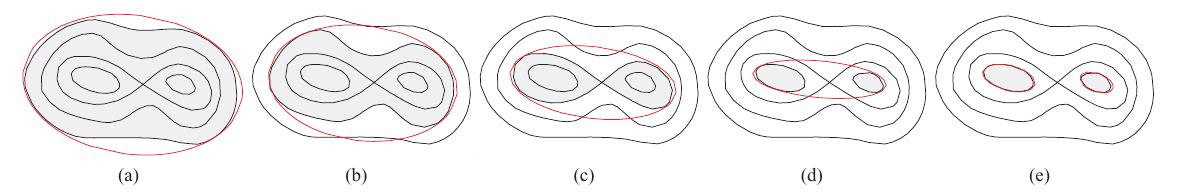
\includegraphics[width=\textwidth]{MultiNest2}
\caption{Cartoon illustrating the MultiNest sampling process. (a) -- (d) show
  the shrinking sampling region with the iso-likelihood contours approximated
  by ellipses. In (e) the sampling region has been separated into two  distinct
  active regions. Figure taken from \cite{MultiNest1}.}
\label{fig:MultiNest_process}
\end{figure} 

The algorithm starts off with evaluating the likelihood values at the initial
ensemble of points in parameter space. From this, an elliptical iso-likelihood
contour is estimated from the points with the lowest likelihoods, as shown in
Fig.~\ref{fig:MultiNest_process}a. Then the contour is scaled down by a certain
factor, Fig.~\ref{fig:MultiNest_process}b, and the points which are now outside
the contour are replaced by new points distributed evenly within the smaller
contour. This procedure is repeated until the likelihood values of all active
points are inside a sufficiently small range, indicating that the maximum has
been found, or the number of iterations has reached the allowed bound.

A powerful feature of the MultiNest algorithm is that it can combine several
overlapping ellipses into one iso-likelihood contour, and hence efficiently map
out irregularly shaped maxima, and even identify sub-samples of active points
belonging to different local maxima. If such sub-samples are detected, the
active region is split into several distinct regions, as shown in
Fig.~\ref{fig:MultiNest_process}e. Then the different regions are optimised in
parallel, and if at some iteration it turns out that one of the local maxima is
significantly lower than the others, the corresponding region gets removed
again.

\begin{figure}[ht]
 \centering
 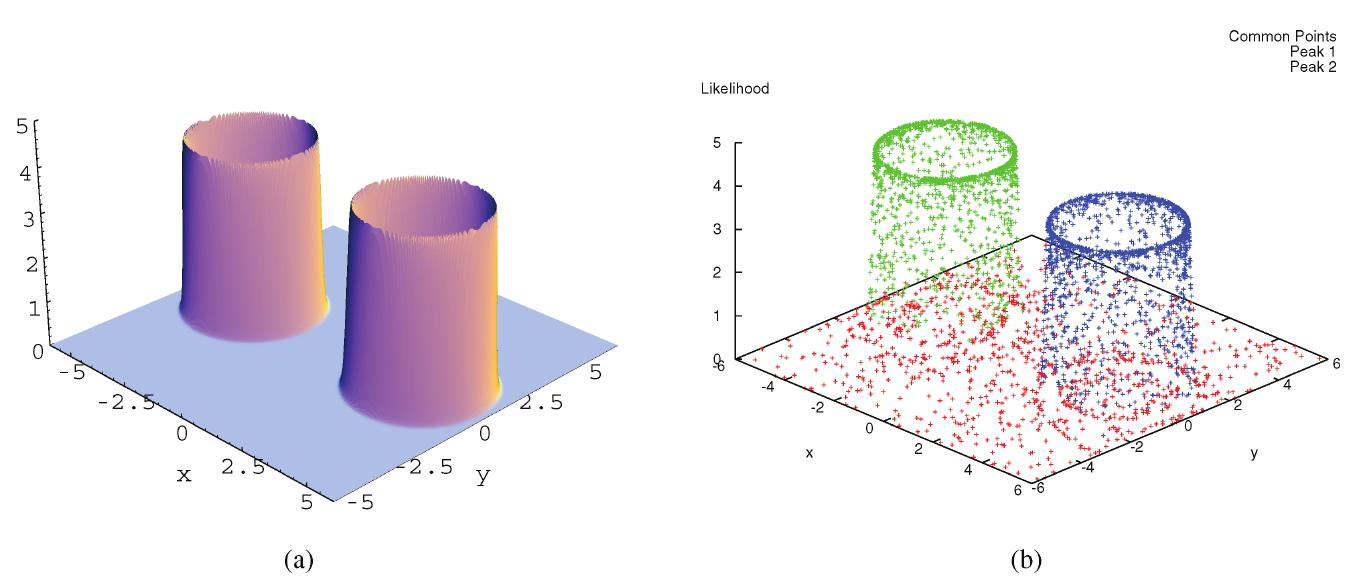
\includegraphics[width=0.8\textwidth]{MultiNest3}
\caption{Example of MultiNest treating a likelihood landscape with two
  distinct, sharp maxima (a). In (b), the starting ensemble of test points is
  shown in red and the maximum likelihood points from the two isolated
  sub-samples evolving during successive iterations of MultiNest in green and
  blue, respectively. Figure taken from \cite{MultiNest1}.}
\label{fig:MultiNest_result}
\end{figure}

Due to these possibilities, MultiNest is suited to find the maximum likelihood
solution of the HybridReco hypothesis for events in PINGU, where sharp and
irregularly shaped maxima commonly occur. Also the ambiguities described above
can be handled reliably via the technique of disjoint samples following two
possible solutions of the problem in parallel. An example showing MultiNest
operating on an artificial likelihood landscape with sharp edges and two
separated maxima is shown in Fig.~\ref{fig:MultiNest_result}.

%==============================================================================
\section{Event Selection}
\label{sec:EvtSel}
%==============================================================================

Since in PINGU the expected rate of neutrino events is in the order of $1 -
2$\,mHz, corresponding to about five neutrinos per hour, while background
events, the vast majority caused by atmospheric muons, will be triggered at
several kHz\footnote{In IceCube, the trigger rate is $\approx 3000$\,Hz.}, an
efficient background rejection algorithm is essential. At the same time, one
has to make sure that a large fraction of the neutrinos carrying the neutrino
mass hierarchy signal pass the imposed cuts---since it is only a second-order
effect event statistics are of great importance---and that the signal in the
data is not destroyed or changed by the cuts.

For the data samples used in this study, a two step selection has been applied
\cite{Processing}. The rationale for this approach is the efficient use of
computing resources. At least the first part of the data reduction has to be run
directly at the South Pole due to the limited bandwidth for data transmission to
the northern hemisphere. Hence the computing for this part has to be
lightweight, as computing resources in Antarctica are scarce as well. After the
easily identifiable background events have been removed, more involved
reconstructions can be run on the remaining data, whose results will be used for
a refined second event selection and eventually in the analysis of the final
data sample.

% \subsection{Trigger and Noise Cleaning}
% \label{sec:cuts_trigger}
% TODO: Write about it?

\subsection{Step 1}
\label{sec:cuts_step1}

The first set of cuts is based on the rather fast CLast and Monopod
reconstructions and on the topology of the charge distribution in the detector
itself. The cut variables have demonstrated their discrimination power in
previous DeepCore analyses, where atmospheric neutrino oscillations have already
been measured at higher energy \cite{DCosc}.

\begin{description}
 \item[$\mathbf{z_\mathrm{CLast} < -200}$\,m:] The very first cut requires the
  event vertex reconstructed by the CLast algorithm to be below --\,200\,m in
  IceCube coordinates, which is 20\,m below the topmost PINGU DOMs. Since
  atmospheric muons enter the detector from above moving downwards, their
  vertices tend to be reconstructed  at the highest possible location while the
  neutrinos that PINGU is interested  in have travelled through the Earth and
  interact inside the detector volume,  pointing upwards.

\item[C2QR6\ $\mathbf{>0.5}$:] The next cut is the so-called ``C2QR6'' quantity
  being  larger than 0.5. It is defined as the fraction of the total PMT charge
  in the  event that has been accumulated within the first 600\,ns, while the
  two very  first hits are ignored. Muons are usually travelling through the
  detector on  an extended path and generate Cherenkov light evenly along it, so
  that usually  only a small fraction of it is recorded during the first
  600\,ns\footnote{During this time, a muon propagates $ct\approx180$\,m.}.
  Neutrinos on the other hand deposit a large fraction of their energy in the
  hadronic cascade that only lasts for few ns.

\item[$\mathbf{z_\mathrm{travel} > -30}$\,m:] For the third cut, the mean spread
  in $z$  of all hits is calculated relative to the mean depth of the first
  quartile of  hits in the event. The cut is passed if this value is larger than
  --\,30\,m,  meaning that the the topology of the event is not too strongly
  pointing  downwards. Again this disfavours muons travelling through the
  detector from  top to bottom while retaining neutrinos coming from below.

\item[$\mathbf{t_\mathrm{90\,\%} < 2}$\,\textmu s:] This cut requires the
  time from  the start of the event after which 90\,\% of the total charge has
  been  accumulated to be less than 2\,\textmu s. Again the reasoning is that
  background muons deposit their energy evenly on their rather long path
  through the  detector, while neutrinos are almost point-like sources in both
  location and  time.

\item[$\mathbf{r_\mathrm{Monopod} < 95}$\,m:] Looking at the secondary 
  Monopod reconstruction, the final cut at the first level secures that the
  event is contained in the detector volume not only vertically, but also
  horizontally. This horizontal containment is considered to be fulfilled if
  the reconstructed vertex is not farther than 95\,m from the detector centre
  at ($50$\,m, $-35$\,m) in the $xy$ direction. The containment assures that
  the event has the possibility to be successfully reconstructed by the
  MultiNest algorithm, which has to be run prior to the second cut level.
\end{description}


\subsection{Step 2}
\label{sec:cuts_step2}

The intention of the second set of cuts is not so much to reject background
events, which is the focus of the first cut level, but rather to select
well-reconstructed events whose quality is sufficient for the final analysis.
Therefore all the cuts in the second step are merely containment cuts, assuming
any non-neutrino event fulfilling the strict containment has already been
recognised and removed in the first step. The reference reconstruction for the
following cuts is the MultiNest reconstruction (Sec.~\ref{sec:reco_multinest})
that has been run on all events passing the first stage of cuts.

\begin{description}
 \item[$\mathbf{-500}$\,m $\mathbf{< z_\mathrm{vertex} < -180}$\,m:] The upper
  bound of the vertical containment, as shown in
  Fig.~\ref{fig:string_layout_side}, has been loosened with respect to the
  $z_\mathrm{vertex} < -200$\,m cut in step one, where the stricter bound was
  necessary due to the strong downgoing background contamination. The lower
  boundary has been introduced since events originating from far below the
  instrumented volume generally have poor reconstruction quality as only
  photons that have travelled far through the ice and hence are subject to
  multiple scattering contribute to the signal recorded in the detector.

 \item[$\mathbf{r_\mathrm{vertex} < 85}$\,m:] The horizontal containment, shown
  in Fig.~\ref{fig:string_layout}, has  been tightened by 10\,m compared to the
  first step. Since the reconstructed  zenith angle of the neutrino is a key
  variable in the mass hierarchy  analysis, one needs to make sure that this
  quantity is reconstructed as accurately as possible. This can not be
  guaranteed for events that are so  close to the edge of the detector that they
  are recorded only partly.

 \item[$\mathbf{\theta_\mathrm{zenith} \geq \pi/2}$ (optional):] For the mass
  hierarchy analysis, neutrinos that have undergone oscillations in a matter
  potential have to be selected. This means that only events that are
  reconstructed as upgoing and hence have passed through the Earth will be
  selected for the final data sample. However, the downgoing neutrino sample
  can still be used as a control region, e.\,g.\ for the normalisation of the
  atmospheric neutrino flux or to estimate the remaining background
  contamination at the final cut level.
\end{description}

\subsection{Particle Flavour Identification}
\label{sec:cuts_PID}

Since in PINGU the main oscillation channels are muon neutrinos converting into
\nue or \nutau, which are all selected by the event selection strategy
described above, it is necessary to reconstruct the flavours of the neutrino
events in the final data sample. As shown in Sec.~\ref{sec:NuDetection},
however, PINGU can only distinguish between track-like events corresponding to
\numu CC interactions with a muon in the final state and cascade-like events,
made up from of \nue and \nutau CC events and NC events of all flavours,
which lack the outgoing muon and consist of a cascade only, and possibly
missing energy in form of an outgoing neutrino.

To make this discrimination as efficient as possible, a boosted decision tree
\cite{BDT} has been set up to generate a single cut variable from the
combination of six input variables, all carrying information on the topology of
the underlying event \cite{PID_BDT}. Three of these variables based on the
distribution of the reduced arrival times with respect to the reconstructed
vertex ($\vec{x},\,t$),
\begin{equation}
 t_i^\mathrm{red} = t_i - t - |\vec{r}_i - \vec{x}|/c \quad,
\end{equation}
of the DOM hits in the event while the remaining three refer to the result of
the MultiNest reconstruction:
\begin{description}
 \item[Early hit charge:] The number of DOM hits in the time window
  [$-200,\,-6$]\,ns (i.\,e.\ before) relative to the reconstructed vertex time.
  Track-like events tend to have a larger number of these early hits since the
  muon travelling through the detector and hence emitting light over a longer
  time causes a bias towards late vertex times. Then direct hits from the
  cascade can be registered prior to the reconstructed interaction vertex
  (cf.~Sec.~\ref{sec:reco_multinest}).
 \item[Very late hit charge:] The number of DOM hits in the time window
  [$200,\,20000$]\,ns relative to the reconstructed vertex time. Track-like
  events tend to have a larger number of very late hits as well, as the total
  light deposition is spread out over a longer time span due to the muon.
 \item[Time to accumulate 10\,\% of the total charge:] In cascade-like events,
  light deposition happens at a more or less singular point in space and time,
  such that the first 10\,\% of the integrated PMT charge are accumulated 
  faster than in spread-out track events.
 \item[Reconstructed muon length:] The propagation length of the
  muon reconstructed by MultiNest before it has deposited all its energy and
  decays. Obviously, this value should be larger for true track events while
  cascades should ideally contain a muon of zero length.
 \item[Muon fractional energy:] The fraction of the total reconstructed energy
  that is accounted to the muon, $\frac{E_\mu}{E_\mu+E_\mathrm{cscd}}$. Similar
  to the above, this is a measure how prominent the muon features are in the
  event and is close to zero for cascades.
 \item[Best vs. cascade-only likelihood:] For the best fit parameters found by
  MultiNest, the likelihood of the cascade-only hypothesis is evaluated by
  setting the muon energy to zero and scaling up the cascade energy accordingly.
  The larger the difference to the actual value of the best-fit likelihood
  including a muon, the more probable that a muon is contained in the event.
\end{description}


%==============================================================================
\section{Next-Generation Optical Modules}
\label{sec:Gen2DOM}
%==============================================================================

Currently two different prototypes of optical modules are supposed to be
deployed in PINGU. The first one, called mDOM (Sec.~\ref{sec:mDOM}), is an
adaptation of the Km3NeT optical module \cite{Km3NeTmodule} whose shape has been
changed from spherical to cylindrical in order to fit into the holes drilled for
the PINGU strings. The other one, called WOM (Sec.~\ref{sec:WOM}), is a novel
approach to enhance the photon collection efficiency by using passive
components.

Both types of modules will be described in more detail below. In
Sec.~\ref{sec:om_effects}, the performance of a PINGU detector consisting fully
of these next-generation modules will be investigated.

\subsection{Multi-PMT Optical Module (mDOM)}
\label{sec:mDOM}

% \begin{figure}[htp]
%  \centering
%  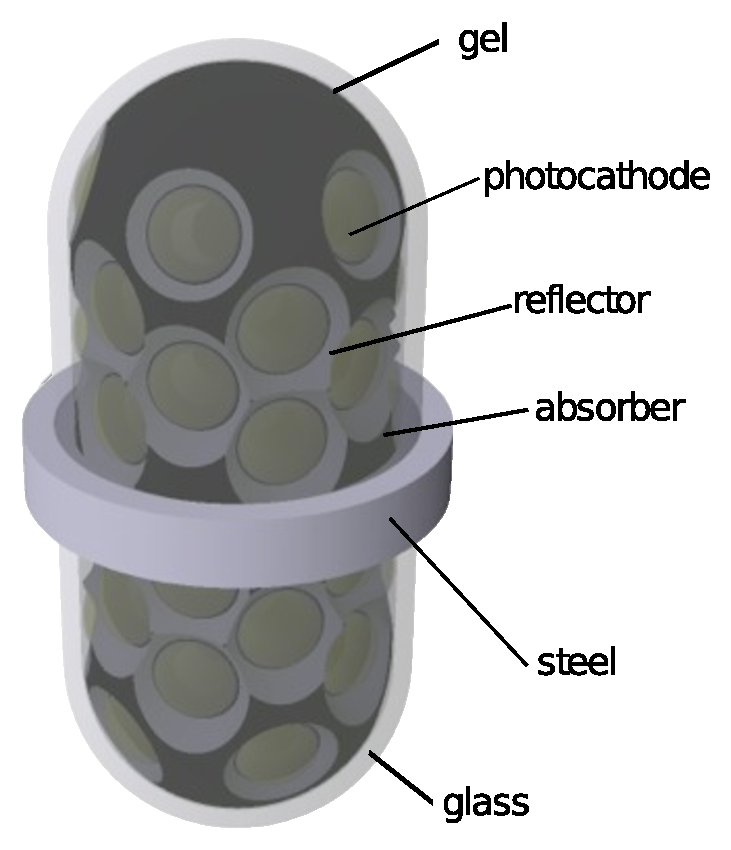
\includegraphics[width=0.5\textwidth]{mDOM_cropped}
%  \caption{The mDOM module concept. Graphics taken from \cite{mDOM_Geneva}.}
%  \label{fig:mDOM}
% \end{figure}

\begin{figure}
\centering
  \subfloat[\label{fig:mDOM}]
    {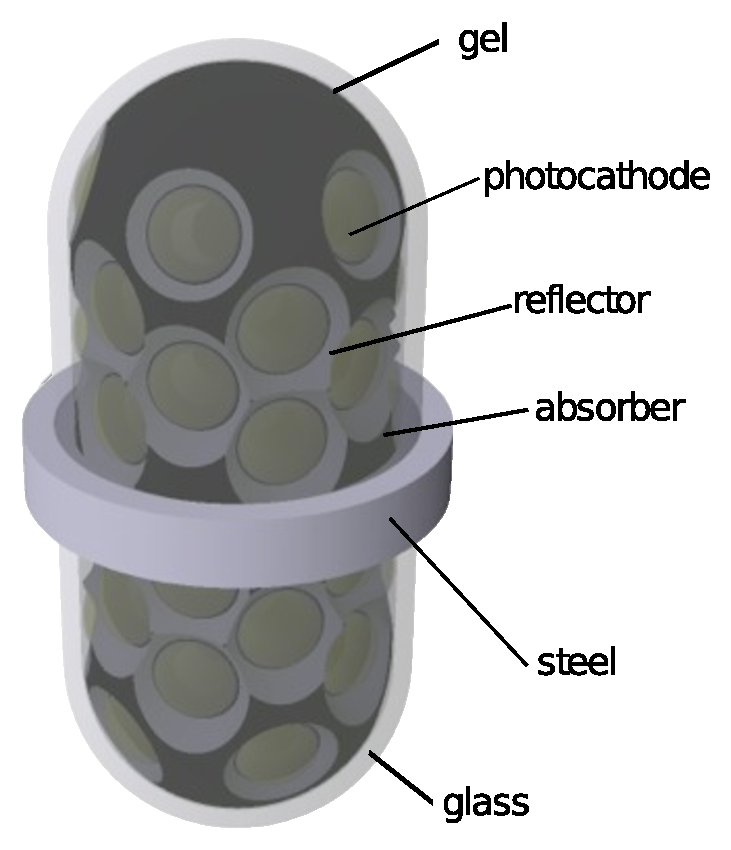
\includegraphics[height=7cm]{mDOM_cropped}}\qquad
  \subfloat[\label{fig:WOM}]
    {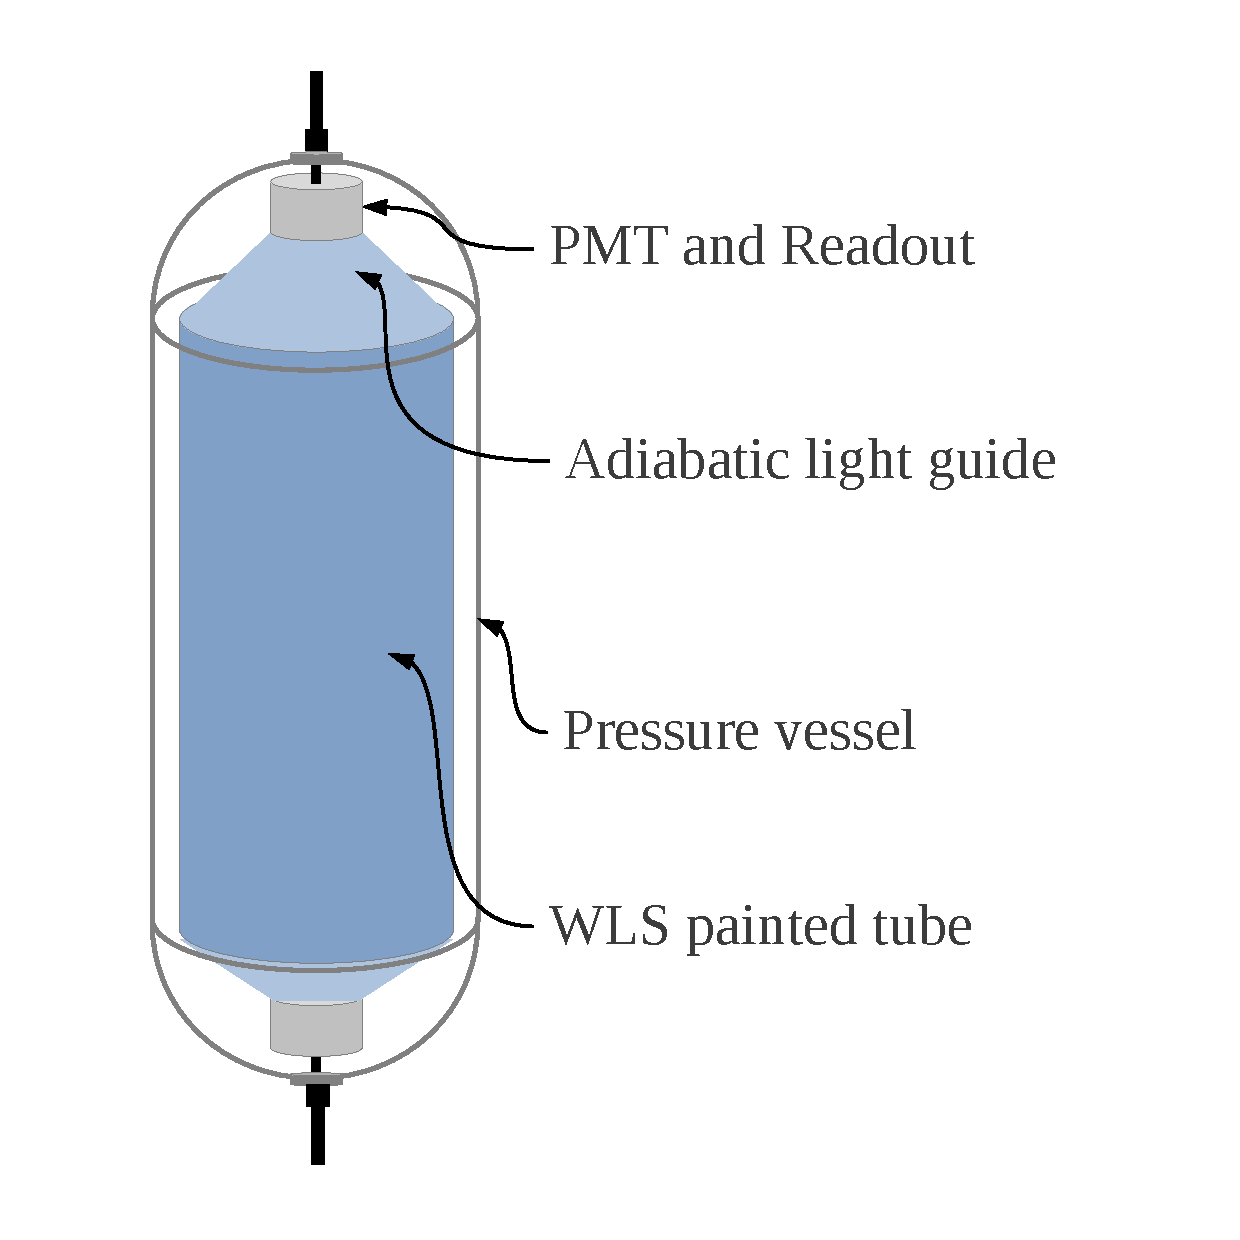
\includegraphics[height=7cm]{WOM}}
  \caption{The \protect\subref{fig:mDOM} mDOM and \protect\subref{fig:WOM} WOM
    module concepts. Graphics taken from \cite{mDOM_Geneva} and \cite{WOM_ICRC},
    respectively.}
\label{fig:Gen3modules}
\end{figure}

Comparing the mDOM, short for Multi-PMT Optical Module, to the standard PINGU
DOMs, the main difference is that instead of one single large PMT, a total of
41 small PMTs with 3\verb+"+ diameter will be used for photon detection, see
Fig.~\ref{fig:mDOM}. The advantages from this layout are that the angular
acceptance covers almost every direction, in contrast to the downwards-pointing
single PMT that has no sensitivity for photons arriving from above
\cite{mDOM_Geneva}.

In addition, the use of more than one PMT per module allows for a very
effective noise reduction. If one only counts module hits where at least two
different PMTs on the same module have registered a photon within a very short
coincidence time, the most important sources of module noise can be strongly
suppressed: Both radioactive decays inside the PMT glass housing and random
electronic noise are restricted to one PMT at a time and hence vetoed with
close to 100\,\% efficiency.

\subsection{Wavelength-shifting Optical Module (WOM)}
\label{sec:WOM}

The WOM on the other hand uses smaller PMTs as well, but enhances the sensitive
area of the module by using passive components as light collectors and
concentrators instead of putting several PMTs into one module \cite{WOM_ICRC}.
The main component, as shown in Fig.~\ref{fig:WOM}, will be a cylindrical tube
made of quartz glass, which has a very low contamination with radioactive
isotopes, that has a coating with wavelength-shifting properties.

In this coating, Cherenkov photons, which are mostly in the UV range (cf.\
Sec.~\ref{sec:Cherenkov}), will be absorbed and then re-emitted isotropically
at a larger wavelength. Due to this isotropic emission a large fraction of the
photons, which were incident roughly perpendicular to the cylinder surface,
will be captured within the tube and hence guided towards its end via multiple
total internal reflection. At the end of the tube, an adiabatic light guide
will project its cross-section area onto a small PMT which then reads out the
photons. Since their spectrum has been shifted from the UV to the optical blue,
it is now better suited for readout by conventional PMTs which are usually most
sensitive for the blue and green part of the optical regime.

In this setup, the size of the sensitive area is given by the coated quartz
glass tube, whose dimensions, especially the length, can be scaled up almost
arbitrarily. At the same time the module noise is dominated by the single PMT
at $\mathcal{O}$(10\,Hz) \cite{WOM_ICRC}, since the quartz glass housing and the
organic wavelength shifter are passive components without electronic noise, and
their radioactive contamination is negligible. So in contrast to the mDOM, the
WOM can fully exploit its large sensitive area to increase the photon
statistics, while in the former the larger sensitive area gets eaten up by the
fact that only multiple photon hits on the same module are counted.

%==============================================================================
\chapter{Simulation}
\label{sec:sim}
%==============================================================================

As this thesis is about estimating the performance of the PINGU detector before
it is actually built, the estimate has to be based on simulations. In the
chapter on hand, the simulations used to generate the results reported in the
following chapter will be described in detail.

The chapter, as the simulation process, is divided into two sections.
Sec.~\ref{sec:sim_MCchain} will discuss the existing and well-established
IceCube Monte Carlo (MC) chain, which has been adopted for PINGU simulations.
Here, individual neutrino events are generated and their output of Cherenkov
photons is modelled. After propagating the photons through the ice, the
resulting hit pattern is processed through the standard reconstruction and event
selection specified in Secs.~\ref{sec:EvtReco} and \ref{sec:EvtSel},
respectively. The outcome of this event-by-event MC, \ie the effective
areas, reconstruction resolutions, and particle identification efficiencies for
all neutrino flavours, are then used as input for the second part of the
detector simulation.

The Parametric PINGU Analysis, \papa in short, was written specifically for the
rapid analysis of PINGU's neutrino mass hierarchy sensitivity including a
variety of systematic parameters. Since propagating these through the full
MC chain would be way too time-consuming, an effective detector
simulation was implemented that, instead of operating on individual events,
generates the expected event distributions directly, based on the detector
performance retrieved from the MC data. \papa will be described in
detail in Sec.~\ref{sec:papa}.

%==============================================================================
\section{The IceCube/PINGU Simulation Chain}
\label{sec:sim_MCchain}
%==============================================================================

\subsection{Event Generation}
\label{sec:MC_genie}

The first step in the MC chain is to model the interaction of an incoming
neutrino with a target nucleus and the resulting final state, the so-called
event generation. In the dedicated PINGU MC, this is carried out using the
GENIE (Generates Events for Neutrino Interaction Experiments) \cite{GENIE}
software package. This is already the first modification of the standard
IceCube MC chain, where NuGen \cite{NuGen}, an IceCube-specific neutrino
generator, is the default. Yet NuGen is laid out for high-energy neutrino
events where only deep inelastic scattering has to be considered as an
interaction process. In PINGU, however, the low GeV energy range is carrying the
interesting oscillation signal, and here the complex interplay between
quasi-elastic and deep-inelastic scattering as well as resonant processes have
to be taken into account (see Sec.~\ref{sec:Xsecs}). Since GENIE puts much
effort into modelling especially this energy range with great care and
validating it against experimental results, it is the natural choice for
generating PINGU events.

GENIE starts off with an isotropic flux of neutrinos of a given flavour
following a user-defined power-law distribution in energy (usually $\propto
E^{-1}$ or $E^{-2}$ for PINGU MC \cite{PINGU_MC}) on the surface of a
cylindrical generation volume well encompassing the full IceCube detector. Any
generated neutrino passing through the interaction volume, which is fully inside
the generation volume but still contains the detector as a whole, is forced to
interact inside this volume. The interaction type is chosen randomly from the
ones that are allowed and the event is assigned a weight $\mathcal{W}_i$
proportional to the particular interaction probability, taking into account the
generated energy spectrum. This weighting strategy makes it possible to
re-weight the generated events to any desired incoming flux $\Phi(E, \theta)$
later on. Then the actual weight is simply given by
\begin{equation}
 w_i = \frac{\Phi(E_i, \theta_i)\,\mathcal{W}_i}{N_\mathrm{evts}} \quad,
 \label{eqn:reweight}
\end{equation}
where $N_\mathrm{evts}$ is the total number of simulated events.

After the interaction mechanism has been determined, the interaction itself is
modelled in detail and all involved particles, from the initial neutrino and
nucleus over possible intermediate states to the final (meta-)stable particles
like pions or muons, are stored inside an \texttt{I3MCTree} object for further
processing. The reference to a tree comes from the fact that this object has
the structure of a multiply nested list, where every particle is the root of a
sub-tree (or branch) holding the particles created in its decay. The particles
are characterised by their identities, positions, four-momenta, and state (such
as 'initial', 'intermediate', or 'final'). 
Additional GENIE-specific information such as the number of generated events,
$N_\mathrm{evts}$, the size of the interaction volume, and others, are kept as
an \texttt{I3MCWeightDict} object.

\subsection{Particle Propagation}
\label{sec:MC_clsim}

The \texttt{I3MCTree} generated by GENIE is handed off to the mmc module
\cite{mmc}, which propagates the final state particles in the tree as well as
possible secondaries created in their decay further through the ice until they
have deposited all their energy. 

\subsection{Detector Response}
\label{sec:MC_detector}

%==============================================================================
\section{The PaPA Code}
\label{sec:papa}
%==============================================================================

\subsection{Idea}
\label{sec:sim_idea}


\subsection{Implementation}
\label{sec:papa_code}


\subsection{Systematic Parameters}
\label{sec:systematics}


%==============================================================================
\chapter{Analysis}
\label{sec:ana}
%==============================================================================

Now that the tools and theoretical foundations needed for the simulation of an
PINGU physics run have been presented and described, the next step is the
actual calculation of PINGU's physics capabilities, in particular its
sensitivity for the neutrino mass hierarchy. This will be done using the Fisher
information matrix, a tool to quickly evaluate the covariance matrix of an
experiment where a large number of systematic uncertainties has to be taken
into account, which will be introduced in Sec.~\ref{sec:fisher}.

Thereafter, the simulation input that was used for the generation of the
results is documented (Sec.~\ref{sec:sim_input}) before finally the results
themselves can be presented and discussed in Sec.~\ref{sec:results_baseline}.
Looking even more into the future, in Sec.~\ref{sec:om_effects} 
the possible benefits of instrumenting PINGU with the next generation optical
modules described in Sec.~\ref{sec:Gen2DOM} will be estimated. Finally, one can
make use of the
Fisher matrix's ability to easily combine the results of different experiments
measuring the same physical effect to evaluate the benefits gained from the
joint analysis of PINGU and other neutrino oscillation experiments, in
particular JUNO \cite{JUNO} (Sec.~\ref{sec:JUNO}). The chapter concludes with a
summary of the findings in Sec.~\ref{sec:ana_summary}.


%==============================================================================
\section{Fisher Information Matrix}
\label{sec:fisher}
%==============================================================================

The Fisher information matrix, or just Fisher matrix in the following, provides
a way to estimate the full covariance matrix of an experiment and therefore the
accuracy of its intended measurement in advance. It has been widely used,
especially in cosmology \cite{Fisher_first}, but also in neutrino
astrophysics \cite{MarekDiffuse}. For a detailed discussion see \eg
\cite{Fisher_first, DETF, DETF2}.

The experiment that is to be modelled is characterised by two sets of variables:
\begin{description}
 \item[Observables] are the variables $f_n$ that will actually be measured by
  the experiment. In the case of PINGU, these are the expected event counts 
  binned in energy and zenith angle. Since the partial derivatives of the
  observables \wrt the parameters enter the calculation of the Fisher matrix,
  their dependence on the parameters has to be known either analytically or (as
  in this analysis) from simulations, such that these derivatives can be
  determined in an analytical or numerical way.
 \item[Parameters] are the variables $p_i$ that will be extracted from the
  measurement (\ie from the observables). These are the physical parameters
  which are the actual target of the experiment as well as nuisance parameters
  required to account for systematic uncertainties.
\end{description}
Then the Fisher matrix is defined as:
\begin{equation}
 \mathcal{F}_{ij} = \sum_n \frac{1}{\sigma_n^2} \frac{\partial f_n}{\partial
p_i} \frac{\partial f_n}
 {\partial p_j}\bigg|_\mathrm{fid.\,model}
 \label{eqn:fisher_def}
\end{equation}
Here the $\sigma_n$ denote the errors on the measurement of the observables.
Since in this analysis, these are the expected numbers of events in the bins $n$
of the analysis histograms (cf.\ Sec.~\ref{sec:papa_code}), $f_n = N_n$, one
can apply Poissonian statistics where the errors are simply given by the square
root of the number of events:
\begin{equation}
 \sigma_n = \sqrt{f_n} = \sqrt{N_n}
\end{equation}
The derivatives in (\ref{eqn:fisher_def}) are evaluated at the set of ''true''
values of $p_i$ that are used as an input for the simulation. This set of
parameters $p_i$ is called the \emph{fiducial model} and is chosen with the best
existing knowledge.

\subsection{Properties}

Once the Fisher matrix has been constructed, the covariance
matrix of the experiment is obtained by inverting the Fisher matrix. Then the
full errors of the parameters $\sigma_i^{\rm full}$ and their correlations can
be read from the covariance matrix $\mathcal{S}$:
\begin{equation}
 \sigma_i = \sigma_i^\mathrm{full} = \sqrt{\mathcal{S}_{ii}}
                        = \sqrt{\left(\mathcal{F}^{-1}\right)_{ii}}
 \label{eqn:sigma_full}
\end{equation}
Also the purely statistical error of a given parameter $\sigma_i^\mathrm{stat}$
(\ie the error that is obtained assuming all other parameters are fixed) can be
calculated from the corresponding diagonal element of the Fisher matrix:
\begin{equation}
 \sigma_i^\mathrm{stat} = \sqrt{\left(\mathcal{F}_{ii}\right)^{-1}}
\label{eqn:sigma_stat}
\end{equation}

External constraints on parameters, so-called \emph{priors}, can easily be
incorporated as well. If parameter $i$ has an prior $\sigma_i^\mathrm{ext}$, it
can simply be added to the corresponding diagonal element of the Fisher matrix:
\begin{equation}
 \mathcal{F}_{ii}^\mathrm{prior} = \mathcal{F}_{ii} +
     \left(\frac{1}{\sigma_i^\mathrm{ext}}\right)^2
\end{equation}
To fix one parameter completely, the corresponding row and column are removed
from the Fisher matrix before inversion.

The Fisher matrix allows not only to read off the full uncertainty of any
parameter and all its correlations with other parameters, but also decompose the
full error into the purely statistical part (\ref{eqn:sigma_stat}) and the
contribution arising from the uncertainties of the other parameters, denoted as
\emph{systematic} error $\sigma_i^\mathrm{syst}$ below:
\begin{equation}
 \sigma^\mathrm{syst}_i =
         \sqrt{\sigma_i^2 - \left(\sigma^\mathrm{stat}_i\right)^2}\quad,
 \label{eqn:syst_error}
\end{equation}
where $\sigma_i$ is calculated without any possible priors on
parameter $i$. The correlation coefficient between two parameters $i$ and $j$
can be calculated as:
\begin{equation}
 c_{ij}
   = \frac{\left(\mathcal{F}^{-1}\right)_{ij}}{\sigma_i \sigma_j}
   = \frac{\sigma_{ij}}{\sigma_i \sigma_j}
 \label{eqn:corr_coeff}
\end{equation}
With this, the error ellipse in the $(p_i,p_j)$ plane can be calculated as
well. Its semi-major and semi-minor axes $a$ and $b$ are given by the
eigenvalues of the $2\times 2$ sub-matrix of the covariance matrix corresponding
to the two parameters,
\begin{equation}
 \mathcal{S}^{(i,j)} =
 \begin{pmatrix}
  \,\sigma_i^2 & \sigma_{ij}\, \\
  \,\sigma_{ij} & \sigma_j^2\,
 \end{pmatrix} \quad,
 \label{eqn:cov_submatrix}
\end{equation}
which are equal to \cite{Fisher_ellipse}
\begin{eqnarray}
 a^2 &=& \frac{\sigma_i^2 + \sigma_j^2}{2} +
         \sqrt{\frac{\left(\sigma_i^2+\sigma_j^2\right)^2}{4}+\sigma_{ij}^2} \\
 b^2 &=& \frac{\sigma_i^2 + \sigma_j^2}{2} -
         \sqrt{\frac{\left(\sigma_i^2+\sigma_j^2\right)^2}{4} + \sigma_{ij}^2} 
\end{eqnarray}
for $\sigma_i > \sigma_j$. Otherwise, the roles of semi-major and semi-minor
axis have to be exchanged. These values have to be scaled by a factor $\alpha$
reflecting the confidence level the ellipse is supposed to represent, \eg
$\mathrm{CL} = 68\,\%$ for a $1\sigma$ ellipse. It can be determined after
\begin{equation}
 \alpha = \sqrt{\mathrm{PPF}_{\chi^2,\,2}(\mathrm{CL})} \quad,
\end{equation}
where $\mathrm{PPF}_{\chi^2,\,2}$ is the \emph{percent point function}---the
inverse of the cumulative distribution function---for the $\chi^2$ distribution
with two degrees of freedom.
The rotation of the ellipse corresponds to the angle $\phi$ between the $p_i$
axis and the eigenvector of the reduced covariance matrix
(\ref{eqn:cov_submatrix}):
\begin{equation}
 \tan 2\phi = \frac{2\sigma_{ij}}{\sigma_i^2 - \sigma_j^2}
 \label{eqn:ell_angle}
\end{equation}
Since the parameters $p_i$ and $p_j$ do not necessarily have the same
dimension, all values in the equations above have to taken as dimensionless,
\ie in units of actual size on a plot. For this reason, (\ref{eqn:ell_angle})
has to be divided by the aspect ratio of the plot before taking the arc tangent.

Another important property of the Fisher matrix is its additivity. As one can
see from (\ref{eqn:fisher_def}), where the total Fisher matrix is given by 
summing the contributions from all observables, one can always add a new
measurement to the ones already accounted for just by adding the respective
Fisher matrices. If there are parameters that only appear in one of the
measurements---\eg the relative atmospheric neutrino flux scale
$r_{\mathrm{flux},\,\nue-\numu}$ that has to be considered in PINGU, but not in
JUNO as the latter relies on reactor neutrinos---the matrix of the experiment
not yet having said parameter is expanded by a corresponding row and column
filled with zeroes: As the measurement does not depend on the new parameter, the
uncertainty on its value as extracted from the measurement
(\ref{eqn:sigma_stat}) is $1/\sqrt{0} = \infty$. The full covariance matrix of
the combination of the two experiments is then simply given by the inverse of
the added Fisher matrices.

\subsection{Prerequisites}
\label{sec:fisher_prereq}

As the simplicity of the Fisher matrix formalism suggests, it is not
universally applicable, but an approximation that is only valid under certain
circumstances. The basic requirement that has to be met is that the fiducial
model, in which the Fisher matrix is constructed, already gives a good
description of the actual ``truth''. There are several criteria to judge
whether this requirement is in fact fulfilled, which turn out to all be
equivalent:
\begin{enumerate}[(a)]
 \item In parameter space, the fiducial and true points have to be close
  enough, such that the dependence of the observables on the parameters,
  $f_n(p_i)$, can be approximated by linear functions. I.\,e.\ the partial
  derivatives $\frac{\partial f_n}{\partial p_i}$ entering in
  (\ref{eqn:fisher_def}) are the same at both points. If this was not the case,
  the experiment's ``response'' to the parameters would be different at the two
  points and hence the fiducial point was not appropriate to make predictions
  about the actual truth.
 \item When constructing the likelihood landscape over the parameter space, such
  that
  \begin{equation}
   \frac{\partial^2\mathcal{L}}{\partial p_i^2}
     = \sum_n \frac{\partial f_n}{\partial p_i}
   \label{eqn:fisher_llh}
  \end{equation}
  with a minimum of $\mathcal{L}$ at the true point, at the fiducial point the
  shape of $\mathcal{L}$ can still be approximated by a parabola with the apex
  at the true point. This ensures that the error ellipses, which are nothing
  else than iso-likelihood contours, are in fact elliptical.
 \item The test statistics of the experiment is Gaussian. This means that the
  likelihood values of an ensemble of pseudo-experiments follow a Gaussian
  distribution, no matter whether they are thrown at the fiducial or at the true
  point. \emph{Throwing a pseudo-experiment} means in this case that
  a possible ``real'' experimental outcome is simulated by generating a 2D
  histogram of events filled with random numbers following a Poisson
  distribution with the means taken from the expected event numbers generated
  with \papa.
\end{enumerate}
% Since the likelihood $\mathcal{L}$ introduced in (\ref{eqn:fisher_llh}) does
% not need to be constructed explicitly, only condition (a) will be checked to
% be fulfilled. This validation can be found in App.~\ref{app:fisher_valid}.
That these conditions are, in fact, fulfilled for the baseline settings of
PINGU is demonstrated in App.~\ref{app:fisher_valid}. As for conditions (b)
and (c) this would require a likelihood evaluation of the full parameter
space\footnote{This is not possible within reasonable computing time, which is
why the Fisher Matrix approach has been chosen in the first place.}, here the
validation is restricted to a case with only two systematic parameters, \dm{31}
and \thet{23}.

\subsection{The Hierarchy Parameter}
\label{sec:fisher_hierarchy}

The Fisher matrix can only handle continuous parameters $p_i$, as the
derivatives of the observables \wrt these parameters enter in
(\ref{eqn:fisher_def}). For this reason the hierarchy parameter $h$ was
introduced in (\ref{eqn:hierarchy_parameter}), making the intrinsically
binary\footnote{By construction it can only be either normal or inverted.}
neutrino mass hierarchy continuous. However it still needs to be demonstrated
that this definition leads to a result that can be interpreted in a meaningful
way.

In \cite{Akhmedov}, a metric is defined that allows to evaluate the sensitivity
of an atmospheric neutrino experiment to the mass hierarchy in terms of
standard \delchisq statistics. For every bin of the final analysis histograms in
($E,\coszen$), a \delchi is defined as
\begin{equation}
 \delchi = \frac{N_\mathrm{NH}-N_\mathrm{IH}}{\sqrt{N_\mathrm{NH}}} \quad.
 \label{eqn:def_delchi}
\end{equation}
The expected significance of the experiment's mass hierarchy measurement is
then given by
\begin{equation}
 \mathcal{S}_{\chi^2} = \sqrt{\sum_\mathrm{bins} \delchisq}
 = \sqrt{\sum_\mathrm{bins}
     \frac{(N_\mathrm{NH}-N_\mathrm{IH})^2}{N_\mathrm{NH}} }\quad.
\end{equation}
With the definition of $h$ according to (\ref{eqn:hierarchy_parameter}), from
the Fisher Matrix the statistical error on $h$ can be retrieved:
\begin{equation}
 \sigma_h^\mathrm{stat} = \sqrt{\left(\mathcal{F}_{hh}\right)^{-1}} \quad,
\end{equation}
with
\begin{equation}
 \mathcal{F}_{hh} = \sum_\mathrm{bins} \frac{1}{\sigma_b^2}
   \frac{\partial N_b}{\partial h} \frac{\partial N_b}{\partial h}
  = \sum_\mathrm{bins} \frac{1}{N_\mathrm{NH}}(N_\mathrm{NH}-N_\mathrm{IH})^2
  \quad.
\end{equation}
As the pure normal and pure inverted hierarchy case correspond to $h=1$ and
$h=0$, respectively, \ie the two cases that have to be distinguished differ by
$1$, the statistical significance (without including any systematic parameters)
retrieved from the Fisher matrix is
\begin{equation}
 \mathcal{S}_\mathrm{Fisher} = \frac{1}{\sigma_h^\mathrm{stat}} 
 = \sqrt{\mathcal{F}_{hh}}
 = \sqrt{\sum_\mathrm{bins}
     \frac{(N_\mathrm{NH}-N_\mathrm{IH})^2}{N_\mathrm{NH}}}
 = \mathcal{S}_{\chi^2} \quad.
\end{equation}
Thus the significances calculated according to \delchisq statistics, where by
construction no systematic parameters are included, and from the Fisher matrix
with explicitly excluding systematics are, in fact, identical.

\subsection{Constructing the Fisher Matrix with \papa}

To construct the Fisher matrix for PINGU primarily means to derive the partial
derivatives entering (\ref{eqn:fisher_def}), \ie the derivatives of the
expected number of events \wrt to all systematic parameters $p_i$ introduced in
Sec.~\ref{sec:systematics} for each bin in the final analysis histograms. In
order to this, for every parameter a set of test points\footnote{Typically
$\approx 10$ different values.} in the vicinity of its fiducial value and \papa
is run for this test point while all other parameters are kept at their fiducial
values.

Then for every bin $b$ in the analysis histograms, the expected bin count $N_b$
is fitted as a function of $p_i$ with a parabola, \ie
\begin{equation}
 N_b^\mathrm{fit}(p_i) = c_0 + c_1\cdot p_i + c_2\cdot p_i^2 \quad.
\end{equation}
The sought-after derivative is then simply given by
\begin{equation}
 \frac{\partial N_b^\mathrm{fit}}{\partial p_i} = c_1 + 2 c_2 p_i 
\end{equation}
with $p_i$ at the fiducial value. As this procedure is repeated for ever
parameter and every bin, it produces all ingredients needed to finally
construct the Fisher matrix.

Here another advantage of the Fisher matrix formalism becomes obvious: since
all systematic parameters are treated independently from each other, adding a
new parameter results only in a small relative increase in computing time.
The parameter space is sampled only along one-dimensional paths aligned with
the parameter axes, thus adding an extra dimension only means adding one path
to the sampling. Hence the time needed to get a result scales only linearly
with the number of parameters taken into account while for algorithms sampling
the full parameter space the scaling is exponential. Using a more graphic
explanation, the Fisher matrix infers the shape of the likelihood landscape by
retrieving a cross-section in each coordinate direction and then ``rotates''
them assuming a parabolic shape.
%==============================================================================
\section{Simulation Input}
\label{sec:sim_input}
%==============================================================================

In this section, the actual values of the inputs required by \papa as described
in Sec.~\ref{sec:papa_code} will be presented as they were used to generate the
results reported in Sec.~\ref{sec:results_baseline}. The detector-related
inputs were extracted from the official PINGU Monte Carlo datasets for geometry
V36\footnote{These are the PINGU Monte Carlo runs 390 for \nue and \nuebar, 389
for \numu and \numubar, and 390 for \nutau and \nutaubar.}.

\subsection{Atmospheric Neutrino Flux}
\label{sec:input_flux}

\begin{figure}[htbp]
 \centering
 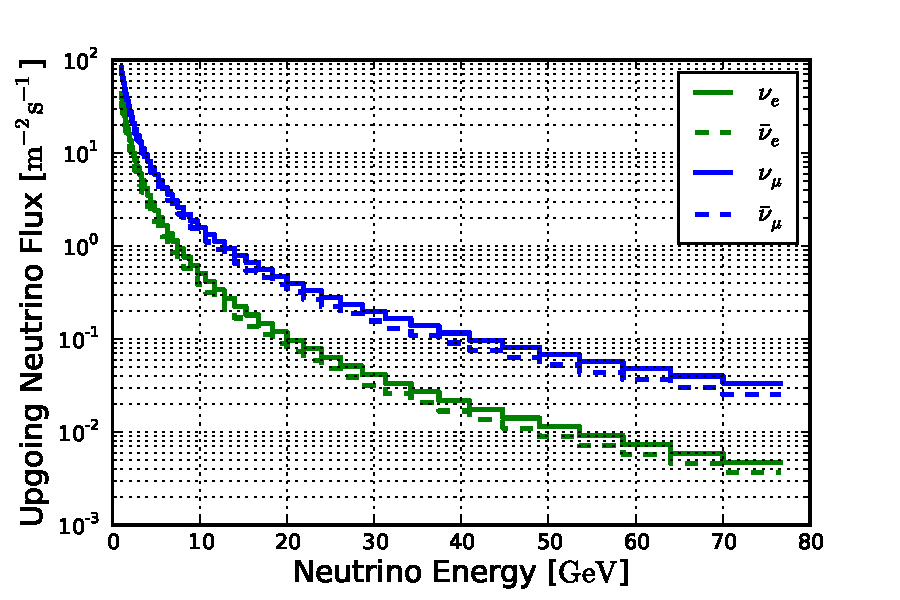
\includegraphics[width=0.7\linewidth]{summed_flux}
 \caption{The atmospheric neutrino flux at the South Pole integrated over all
          upgoing (\coszen in $[-1,0]$) directions. Based on the
          azimuth-averaged neutrino flux tables from \cite{HondaSP}.}
\label{fig:summed_flux}
\end{figure}

As already mentioned, the incoming atmospheric neutrino flux without
oscillations is calculated from the 2014 re-calculation of the flux tables
published by Honda et al.\ \cite{Honda, HondaSP}. A plot of the flux in the
energy range covered by the PINGU simulation (1\,--\,80\,GeV) is shown in
Fig.~\ref{fig:summed_flux}. The flux has been integrated over all upgoing
(\coszen in $[-1,0]$) directions, as downgoing neutrinos arriving from above
the detector do not pass through a significant amount of matter and hence do
not bear any information on the neutrino mass hierarchy.

\subsection{Oscillation Probabilities}
\label{sec:input_osc}

The neutrino oscillation probabilities have been calculated using the
AtmoWeights code for the PREM Earth density profile as described in
Sec.~\ref{sec:PINGUosc}. The fiducial values of the mixing parameters used for
the calculation follow the global fit of Fogli et al.\ \cite{Fogli}, listed in
Tab.~\ref{tab:fiducial_osc}. Example plots of the probabilities demonstrating
the characteristic signature of the mass hierarchy are shown in high resolution
in that section as well, the full set of all possible oscillation channels can
be found in App.~\ref{app:oscillation}. The binning of those plots is the same
as used for the actual analysis, which is 79 logarithmic bins in energy between
1\,GeV and 80\,GeV and 20 equally sized bins between -1 and 0 in \coszen.

\subsection{Effective Areas}
\label{sec:input_aeff}

\begin{figure}[htbp]
 \centering
 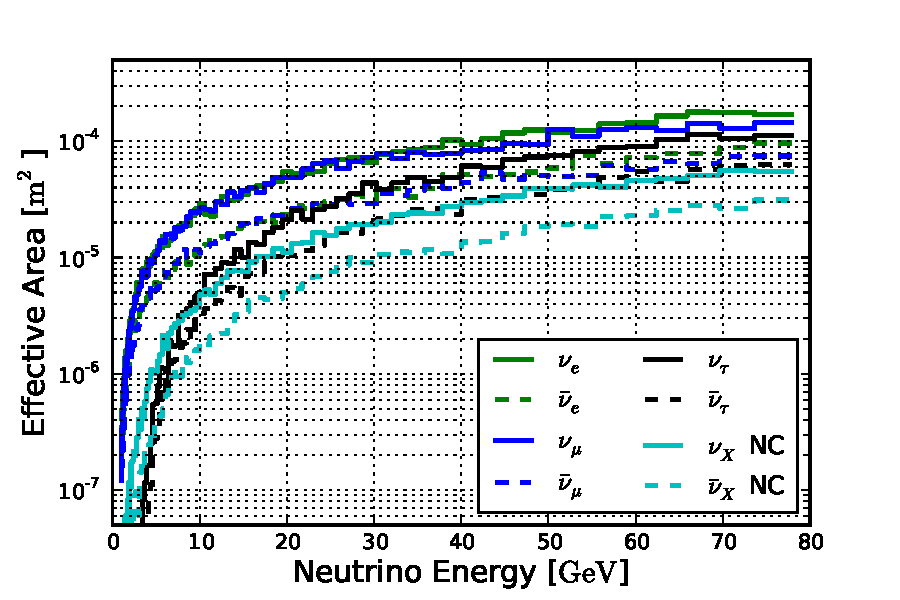
\includegraphics[width=0.495\linewidth]{aeff_energy}
 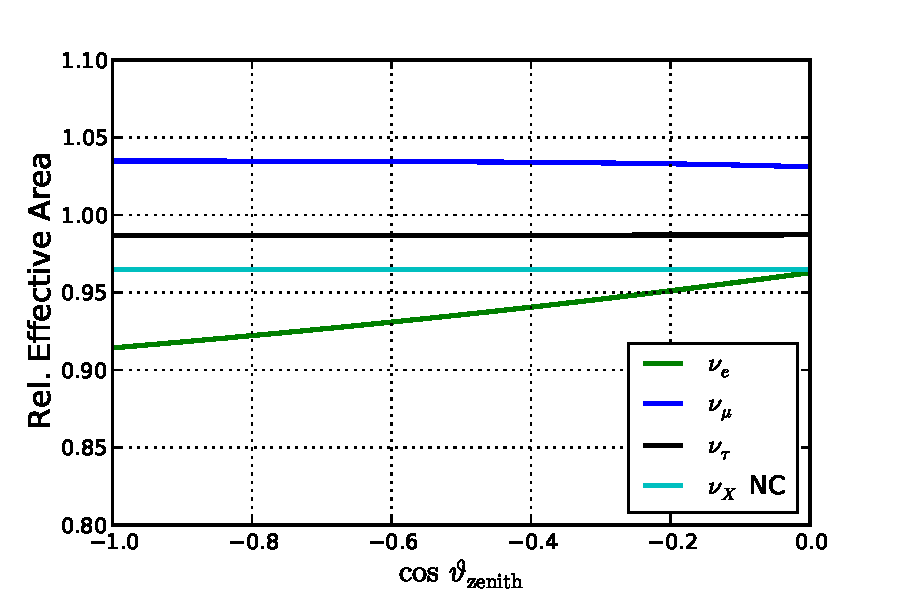
\includegraphics[width=0.495\linewidth]{aeff_coszen}
 \caption{Effective areas for all relevant neutrino interactions. Shown are
  energy (left)  and zenith (right) dependence.}
\label{fig:aeffs}
\end{figure}

The effective areas are extracted from PINGU Monte Carlo datasets via the
OneWeight quantity multiplied by $4\pi$, which is equivalent to a per-event
effective area \cite{OneWeight}. The zenith dependence of the effective area is
modelled by an analytic fit to the MC data, assuming that energy and zenith
dependence can be handled separately. A plot of the effective areas and their
zenith dependence is shown in Fig.~\ref{fig:aeffs}.

\subsection{Reconstruction Resolutions}
\label{sec:input_reco}

As already mentioned, the event reconstruction for the baseline model will be
simulated by 


% \begin{figure}
%  \centering
%  \includegraphics[width=0.495\linewidth]{figures/MultiNest_EnergyResolution.pdf}
%  \includegraphics[width=0.495\linewidth]{figures/MultiNest_ZenithResolution.pdf}
%  \caption{Median resolutions of the \textsf{MultiNest} algorithm for
%   $\nu_e/\bar\nu_e$ and $\nu_\mu/\bar\nu_\mu$ CC events.
%   \emph{Left:} Relative energy resolution.
%   \emph{Right:} Zenith angle resolution}
%  \label{fig:MultiNest}
% \end{figure}


The input for the reconstruction resolutions, whether supplied as
parametrisations or tables, is obtained from the
\textsf{MultiNest}\footnote{Developed by J.\,P.\ A.\,M.\ de Andr\'{e},
M.\ Dunkman, and F.\ Huang (Penn State)} reconstruction algorithm. This 8D
hybrid likelihood minimization fits for the hadronic interaction vertex plus an
outgoing muon. Median resolutions in energy and zenith angle are shown in
Fig.~\ref{fig:MultiNest}.

\subsection{Particle Flavour Identification}
\label{sec:input_pid}

\begin{figure}[htbp]
 \centering
 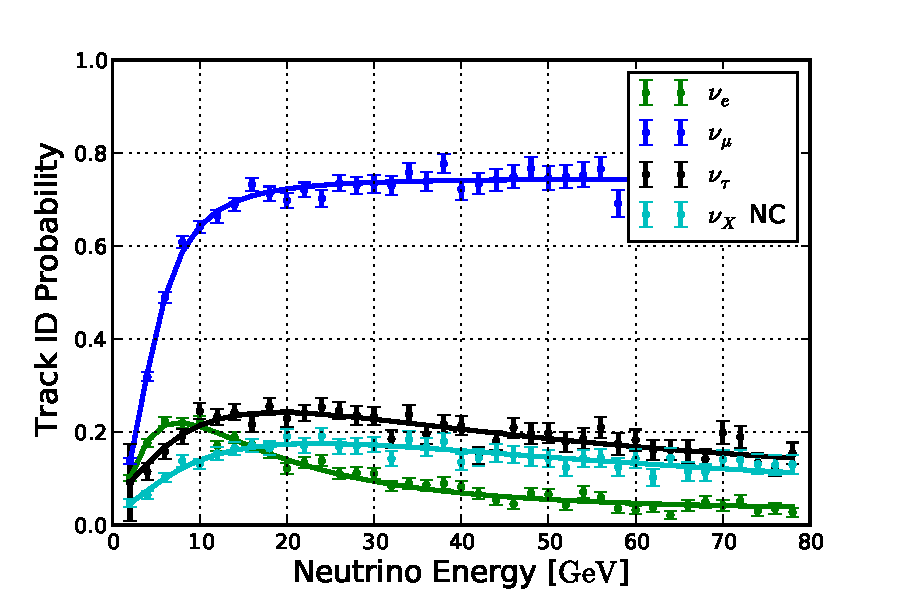
\includegraphics[width=0.7\textwidth]{PID}
 \caption{Track identification probability as function of energy in all four
  interaction channels. The straight lines show fits to the data.}
 \label{fig:PID}
\end{figure}

The classification of the neutrino events into track-like and cascade-like
events is according to their final score in the boosted decision tree described
in Sec.~\ref{sec:cuts_PID}. In the baseline detector settings, the decision is
of binary nature, meaning that the probability to classify a given event as
cascade is one minus the probability to classify it as a track.

Data points for the track identification probabilities in all channels as a
function of the neutrino energy have been provided by \cite{JP_PID}. These data
were fitted with analytic functions, the fits are shown together with the data
points in Fig.~\ref{fig:PID}. The functions definitions themselves are listed
in App.~\ref{app:pid}.
%==============================================================================
\section{Results for the Baseline Geometry}
\label{sec:results_baseline}
%==============================================================================

\begin{table}[htpb]
 \caption{Uncertainties on all systematic parameters for the baseline
  detector model with three years of lifetime, ranked according to their impact
  on the mass hierarchy parameter $h$.}
 \label{tab:baseline_results}
 \begin{center}
  \small{\begin{tabular}{lrrrrrr} 
\toprule
Parameter & Impact [\%] & Best Fit & $\sigma^\mathrm{full}$ & $\sigma^\mathrm{stat}$ & $\sigma^\mathrm{syst}$ & Prior \\ 
\midrule
$h$ & 100.0 & \num{1.00e+00} & \num{3.43e-01} & \num{2.33e-01} & \num{2.52e-01} & free \\
$r_{A_\mathrm{eff},\,\nu-\bar\nu}$ & 8.9 & \num{0.00e+00} & \num{4.73e-02} & \num{4.76e-03} & \num{1.47e-01} & \num{5.00e-02} \\
$\vartheta_{13}$ [$^\circ$] & 8.0 & \num{8.93e+00} & \num{4.64e-01} & \num{8.24e-01} & \num{3.67e+00} & \num{4.68e-01} \\
$n_{A_\mathrm{eff}}$ & 7.4 & \num{0.00e+00} & \num{1.94e-02} & \num{1.99e-03} & \num{1.94e-02} & \num{2.00e-01} \\
$\vartheta_{23}$ [$^\circ$] & 3.2 & \num{3.86e+01} & \num{4.67e-01} & \num{3.02e-01} & \num{3.97e-01} & \num{1.32e+00} \\
$\Delta m^2_{31}$ [eV$^2$] & 2.7 & \num{2.46e-03} & \num{6.49e-05} & \num{1.77e-05} & \num{1.10e-04} & \num{8.00e-05} \\
$r_{\Phi,\,\nu_e-\nu_\mu}$ & 2.4 & \num{0.00e+00} & \num{1.10e-02} & \num{5.12e-03} & \num{1.01e-02} & \num{5.00e-02} \\
$s_{A_\mathrm{eff}}$ [m$^2$/GeV] & 1.1 & \num{0.00e+00} & \num{2.19e-04} & \num{1.23e-04} & \num{1.82e-04} & free \\
$\Delta_\mathrm{PID}$ [GeV] & 0.9 & \num{0.00e+00} & \num{1.70e-02} & \num{1.58e-02} & \num{6.23e-03} & \num{5.00e-01} \\
$s_E$ & 0.1 & \num{1.00e+00} & \num{2.81e-02} & \num{7.66e-03} & \num{3.31e-02} & \num{5.00e-02} \\
\bottomrule 
\end{tabular}
}
 \end{center}
\end{table}

Using the settings described in the previous section, the Fisher matrix for
PINGU can now be constructed with \papa. The full, statistical, and systematic
errors are for all parameters are listed in Tab.~\ref{tab:baseline_results} for
a nominal PINGU lifetime of three years. The parameters are ordered after their
\emph{impact} on the mass hierarchy parameter $h$, which is defined as the
square of their correlation coefficient $c_{ih}$ (\ref{eqn:corr_coeff}) with
$h$. Note that for the baseline settings, the systematic parameter
$s_\mathrm{PID}$ has been excluded as it is fully degenerate with $n_{\aeff}$:
since the PID decision is binary, no channel of unidentified events exists and
hence both parameters just evenly increase the overall number of events,
effectively.

From the first line of Tab.~\ref{tab:baseline_results}, one can read off the
expected significance of PINGU's mass hierarchy measurement by inverting the
full error (see Sec.~\ref{sec:fisher_hierarchy}). This gives an expected
significance of 2.9\,$\sigma$ after three years. Looking at the statistical
error alone, this value increases to 4.3\,$\sigma$, emphasising the important
role systematic parameters are playing in the determination of the mass
hierarchy.

\begin{figure}[bhtp]
 \centering
 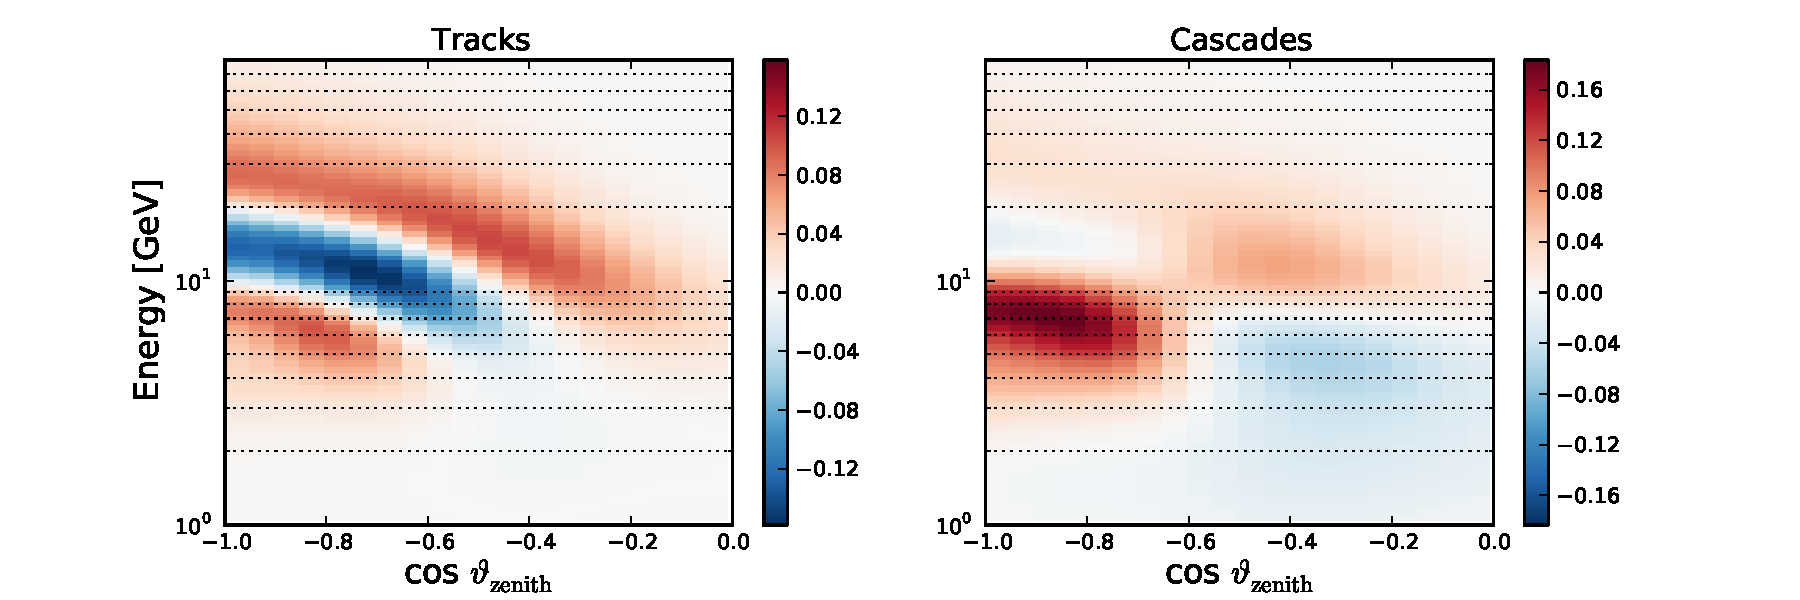
\includegraphics[width=\linewidth]{akhmedov_baseline}
 \caption{\delchi distribution in the track (left) and cascade (right) channels 
for the baseline settings.}
 \label{fig:akhmedov_baseline}
\end{figure}

\begin{figure}[thp]
 \centering
  \subfloat[\label{fig:sigma_vs_time}]
   {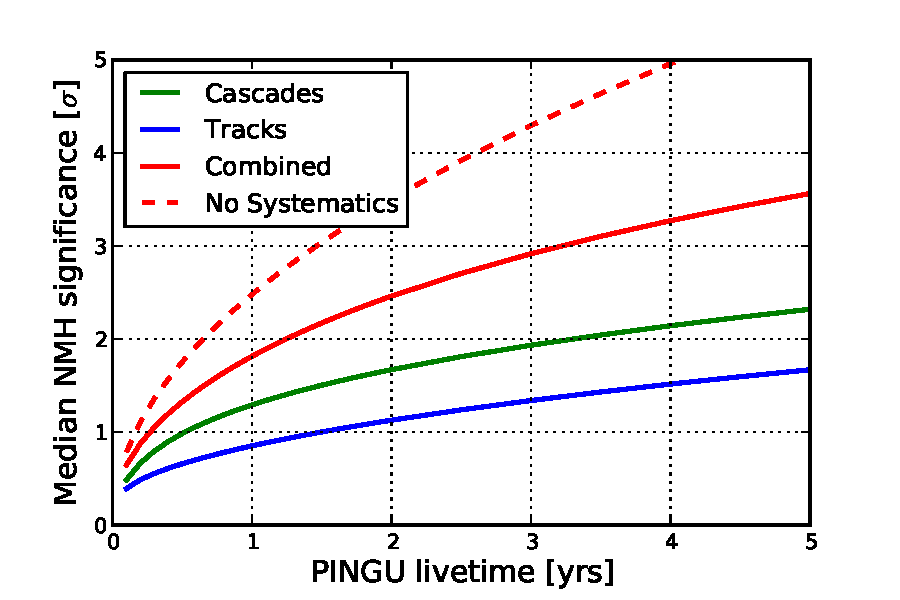
\includegraphics[width=0.495\linewidth]{sigma_vs_time_default}}
  \subfloat[\label{fig:covmat_baseline}] 
   {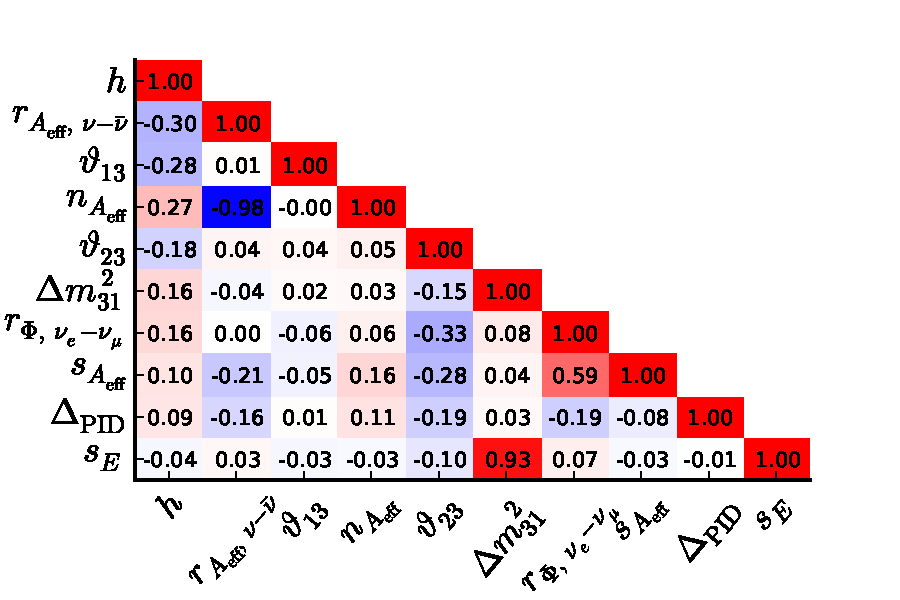
\includegraphics[width=0.495\linewidth]{CovMat_PINGU}}
 \caption{\protect\subref{fig:sigma_vs_time} Evolution of PINGU's expected mass 
          hierarchy significance with time and 
          \protect\subref{fig:covmat_baseline} Full correlation matrix for PINGU
          for the baseline settings.}
 \label{fig:time_covmat}
\end{figure}

Treating the track and cascade channels separately, the expected significances
are 1.9\,$\sigma$ with and 3.0\,$\sigma$ without systematics for the cascade
and 1.3\,$\sigma$ (3.1\,$\sigma$) for the track channel,
respectively\footnote{The full error listings corresponding to
Tab.~\ref{tab:baseline_results} can be found in
App.~\ref{app:fisher_baseline}}. Although the purely statistical significances
are comparable, when taking systematics into account the significance for the
cascades remains much higher than the track significance. 
The reason for this becomes obvious when looking at the \delchi distributions 
for both channels in Fig.~\ref{fig:akhmedov_baseline}. In the track channel, 
there are three distinct regions driving the expected significance. These 
regions are separated only by small margins and have alternating sign, while in 
the cascade channel most of the significance comes from one contiguous region. 
Together with the fact that the cascade channel has roughly three times higher 
event statistics than the track channel---62,000 vs.\ 22,000 neutrino events 
per year---this makes the cascade channel much more robust against the impact 
of systematic parameters.

In Fig.~\ref{fig:sigma_vs_time}, the significances for the individual channels 
and for their combination are shown as a function of time. The purely 
statistical significance is plotted as well, exhibiting a scaling with the 
square root of the lifetime as one would expect for a counting experiment where 
the relative error is proportional to $1/\sqrt{N}$. The actual significances 
including systematics increase much slower with time as a part of the 
accumulating statistics has to be ``spent'' in order to better constrain the 
systematic parameters. However the combined analysis of the two channels still 
gives a much higher sensitivity than simply adding the two individual channels 
in quadrature as one would do for two completely unrelated measurements of the 
same quantity. E.\,g.\ for a lifetime of three years as above, the quadratic 
sum of the track and cascade significances is $\sqrt{(1.3\,\sigma)^2 + 
(1.9\,\sigma)^2} \approx 2.3\,\sigma$, considerably lower than the 
2.9\,$\sigma$ for the combined analysis.

Finally one can look at the correlation matrix of PINGU. In contrast to the 
error listing for all parameters as in Tab.~\ref{tab:baseline_results}, here the 
interdependences between the parameters are in the focus. The graphical 
representation in Fig.~\ref{fig:covmat_baseline} shows, for every combination 
of parameters, their correlation coefficient $c_{ij}$. Using these quantities 
instead of the entries $\sigma_{ij}$ of the covariance matrix themselves has 
the benefit that due to their normalisation, cf.~(\ref{eqn:corr_coeff}), the 
entries of the matrix are dimensionless and restricted to the range $[-1, +1]$, 
thus making them easier to interpret.

From the correlation matrix itself, several things can be learned. First, the 
hierarchy parameter is the one with strongest overall correlations. This 
emphasises the fact that the determination of the neutrino mass hierarchy is a 
very delicate measurement relying on a small effect, and that the inclusion of 
so many systematic parameters is indeed necessary to get a robust result.

\begin{figure}[thp]
 \centering
 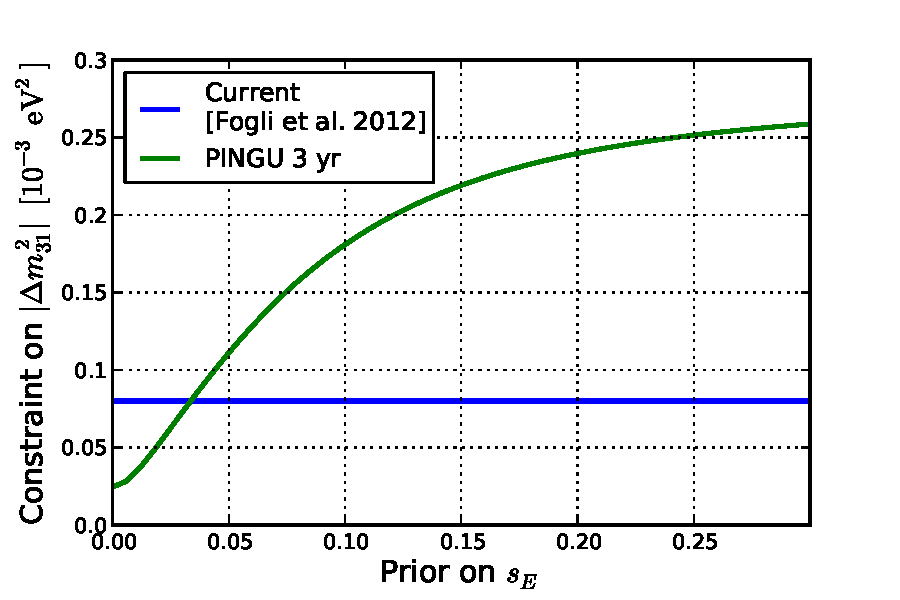
\includegraphics[width=0.7\linewidth]{dm31_vs_escale_prior}
 \caption{PINGU constraint on \dm{31} as a function of the prior on the energy
          scale. No prior knowledge about \dm{31} is assumed.}
 \label{fig:dm31_vs_escale_prior}
\end{figure}

Furthermore, two combinations of parameters stick out due to their very strong 
correlation. The first one is the relative normalisation of the effective areas 
for \nux and \nuxbar, $r_{\aeff,\,\nu-\bar\nu}$, and the overall normalisation 
of all effective areas, $n_{\aeff}$. Their anticorrelation is obvious from 
their definition: $r_{\aeff,\,\nu-\bar\nu}$ increases the number of neutrino 
events while decreasing the number of antineutrino events. Since PINGU cannot 
distinguish between those and the cross-section for neutrinos is higher 
approximately by a factor of two (see Fig.~\ref{fig:NuXsec_GeV}), the total 
number of events is increased, which can be compensated by decreasing 
$n_\aeff$. Only the MSW resonance oscillation causes an asymmetry between 
neutrinos and antineutrinos, such that the anticorrelation is not exactly $-1$.

The second strong correlation can be observed between the absolute value of the 
mass splitting \dm{31} and the energy scale $s_E$. The value of \dm{31} is 
determined from the position of the oscillation minimum in the track channel 
that is easy to spot in Fig.~\ref{fig:SimSteps}. In a two-flavour approximation, 
this can be described by equation (\ref{eqn:osc_length}), where the oscillation 
length is determined by the zenith angle. Then \dm{31} is inversely 
proportional to the neutrino energy. Thus a larger value of \dm{31} can be 
compensated by increasing the energy scale accordingly.

This means that if PINGU is supposed to make a precise measurement of \dm{31}, 
the energy scale has to be known very accurately. As the energy of a neutrino 
event is determined primarily from the number of detected photons\footnote{The 
Cherenkov light output is directly proportional to the deposited energy.}, this
means that the photon detection efficiency of the optical modules has to be
well calibrated. This behaviour is illustrated in
Fig.~\ref{fig:dm31_vs_escale_prior}, where PINGU's self-contained constraint on
the value of \dm{31} is plotted against the prior put on $s_E$. To improve on
the current limits, the energy scale has to be known with an accuracy of at
least 3\,\%.

\subsection{Measuring the Atmospheric Mixing Parameters}
\label{sec:results_atmosperic}

\begin{figure}[thp]
 \centering
 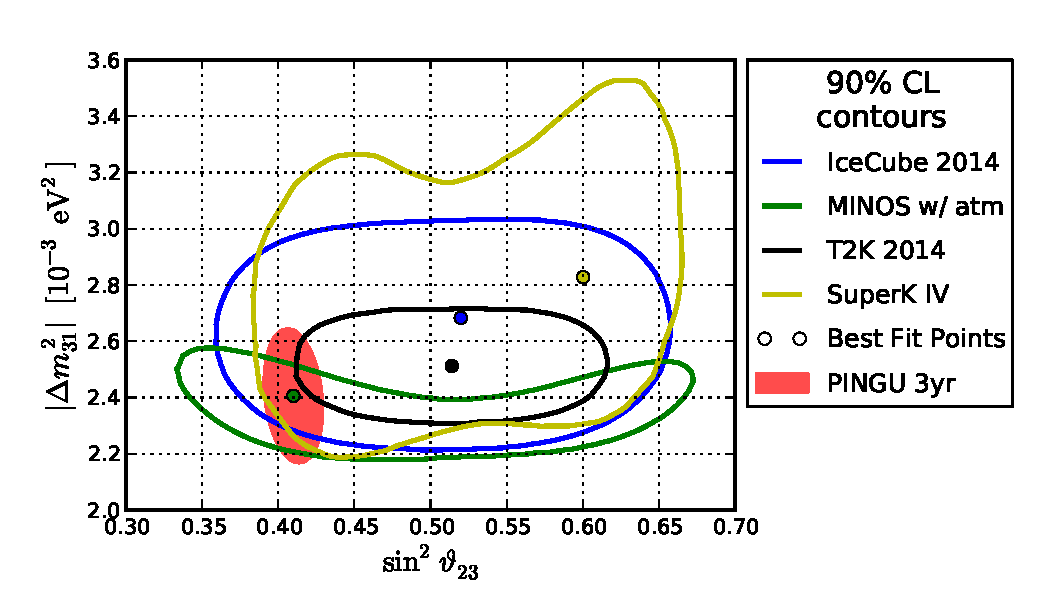
\includegraphics[width=0.85\linewidth]{AtmoParamsBaseline}
 \caption{PINGU constraint on \dm{31} and $\sin^2\thet{23}$ for the baseline
          settings. No prior knowledge about the two parameters is assumed.
          The latest constraints from the IceCube/DeepCore \cite{DCosc}, MINOS
          \cite{MINOSparams}, T2K \cite{T2Kparams}, and SuperKamiokande
          \cite{SuperKparams} are shown for reference.}
 \label{fig:AtmoParamsBaseline}
\end{figure}

To determine the neutrino mass hierarchy, PINGU makes a precision measurement
of the oscillations of atmospheric neutrinos. In fact, with more than 80,000
events recorded per year it will collect the largest sample of atmospheric
neutrinos so far. After DeepCore has been established as a serious contributor
to the global effort of characterising neutrino oscillations, PINGU will go
even further into that direction and provide tight constraints on the values of
\dm{31} and \thet{23}.

These constraints are shown in Fig.~\ref{fig:AtmoParamsBaseline}, along with
the most recent confidence regions of current oscillation experiments. For
PINGU, no priors have been put on \dm{31} or \thet{23}, meaning that the
displayed confidence ellipse comes from PINGU data alone and does not profit
from external knowledge.

The most obvious feature of PINGU's confidence ellipse is its orientation,
which is different from the other experiments: While it cannot constrain
\dm{31} any better than current experiments, the value of \thet{23} will be
much more precise than any measurement available today. The reason for this is
that the value of \dm{31} is extracted from the position of the oscillation
minimum in energy, which needs a precise calibration of the energy scale as we
have seen above. This is much easier to achieve in experiments on a neutrino
beam like MINOS or T2K where the beam energy is well-known. \thet{23} on the
other hand is determined from the relative depth of the oscillation minimum as
one can see from equation (\ref{eqn:twoflavour_prob}). Here PINGU profits from
its wide energy range including control regions without oscillations and the
large event statistics, such that especially the overall detector
efficiency\footnote{Represented by $n_\aeff$ in \papa.}, which usually is
difficult to constrain in beam experiments, only has minor impact.

\subsection{Impact of the Octant of \thet{23}}
\label{sec:results_octant}

\subsection{High-Purity Event Classification}
\label{sec:results_includeunkn}

\subsection{The Missing Monte Carlo Effect}
\label{sec:results_mcstats}


%==============================================================================
\section{Effects of Advanced Optical Modules}
\label{sec:om_effects}
%==============================================================================

In Sec.~\ref{sec:Gen2DOM}, two different concepts to substantially improve the 
optical modules have been introduced, prototypes of both are supposed to be 
deployed in PINGU: the mDOM that has several small PMTs instead of a single 
large one, and the WOM, where the effective area of a single small PMT is 
enhanced drastically by passive components. In this chapter, PINGU will be
modelled as it was built completely from these next-generation optical modules. 
Then the possible benefits for the experiment's outcome can be analysed.

\subsection{WOM: Increasing the Photon Statistics}
\label{sec:wom_effect}

With its enhanced photosensitive area, the WOM will primarily increase the
number of photons detected per event. Since this is the driving parameter for
event reconstruction quality---the more photons are detected, the more
information is available for the reconstruction algorithm---more precise
reconstructions are expected especially at low energies, where photon
statistics are scarce.

To simulate the improvement resulting from a photon count increased by a factor
\phfac in \papa, the \emph{absolute} widths of the energy reconstruction
functions that are usually given by linear functions of the form
\begin{equation}
 \sigma_E( E) = a  E + b \quad,
\end{equation}
where $a$ and $b$ are constants determined by a fit (see
App.~\ref{app:reco_params}), are replaced by
\begin{equation}
 \sigma'_E( E) = a  E + b/\phfac \quad.
\end{equation}
The rationale behind this is that the \emph{relative} energy resolution is
assumed to be a function of the number of detected photons, which in turn is
directly proportional to the neutrino energy\footnote{The number of Cherenkov
photons is proportional to the total deposited energy, see
Sec.~\ref{sec:Cherenkov}.}. Thus increasing the number of detected photons by
\phfac means that an an event with the energy $E$ will now have the relative
energy resolution of an event of energy $\phfac\cdot E$:
\begin{eqnarray}
 \frac{\sigma'_E( E)}{ E} &=& \frac{\sigma_E(\phfac E)}{\phfac E}
  = \frac{a \phfac E + b \quad}{\phfac E} \\
  \Rightarrow \sigma'_E( E) &=& a  E + b/\phfac
\end{eqnarray}
For the \coszen resolution, the modification is more straightforward as one can
simply read out the parametrisations for the absolute widths at an energy
increased by the factor \phfac:
\begin{equation}
 \sigma'_{\cos\theta}(E) = \sigma_{\cos\theta}(\phfac\cdot E) \quad.
\end{equation}

\begin{figure}[thp]
 \centering
 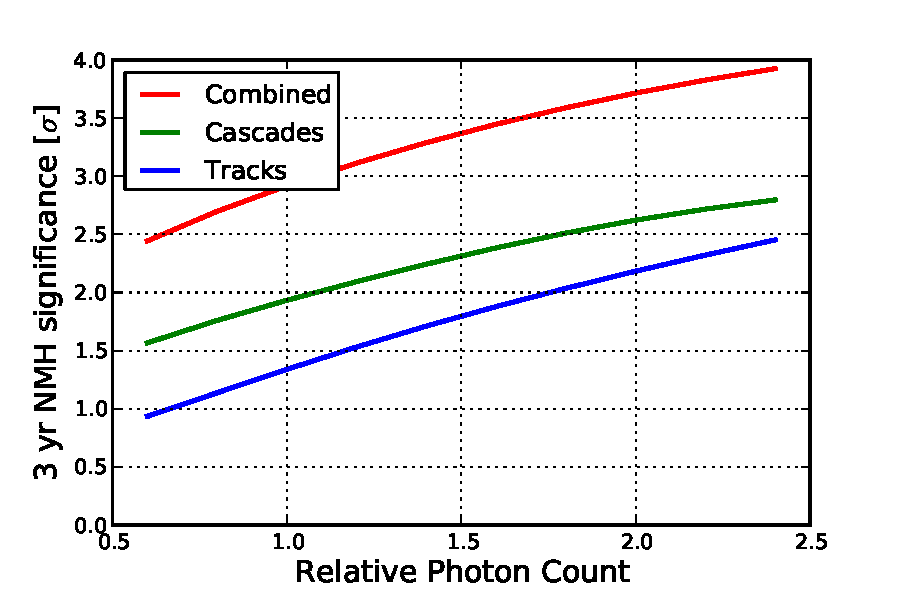
\includegraphics[width=0.7\linewidth]{increase_photon_count}
 \caption{Relative expected three-year significance for the mass hierarchy
          as a function of \phfac.}
 \label{fig:increase_photon_count}
\end{figure}

In addition, the threshold for passing PINGU's event selection is expected to
become lower with an increasing number of photons per neutrino energy,
enhancing the event statistics at low energy. This effect is mimicked by scaling
the effective area at a given energy $E$ by the ratio of the selection
efficiencies $\varepsilon_\mathrm{sel}$ (as shown in
Fig.~\ref{fig:selection_eff}) at $E$ and $\phfac \cdot E$:
\begin{equation}
 \aeff'(E) = \aeff(E) \cdot \frac{\varepsilon_\mathrm{sel}(\phfac\cdot E)}
                                 {\varepsilon_\mathrm{sel}(E)}
\end{equation}
The scaling is applied for all flavours except from \nutau and \nutaubar CC
events, as there the main feature is the kinematic cutoff due to the large mass
of the tau lepton (cf.\ Sec.~\ref{sec:cuts_step2}), which of course is
independent from the performance of the optical modules used in the detector.

This gives a conservative estimate as only effects after the actual triggering
of the detector are taken into account. Since the trigger condition essentially
is a certain number of photon hits being registered within a short time window,
the trigger threshold itself does sink as well, enhancing the overall effect.
Yet as the available amount of MC events before triggering is insufficient to
quantify this, the reduced trigger threshold will be neglected.

% Finally, a similar reasoning can be applied for the particle identification
% efficiency, thus the PID functions will be read off at the scaled energy as
% well:
% \begin{equation}
%  P'_\mathrm{PID}(E) = P'_\mathrm{PID}(\phfac\cdot E)
% \end{equation}

The median three-year significance for the mass hierarchy is shown as a
function of \phfac in Fig.~\ref{fig:increase_photon_count}. As expected, the
mass hierarchy significance increases with the photon statistics as a result of
the improved resolutions and enhanced effective area. When the photon
statistics are doubled, \ie $\phfac =
2$, it reaches 3.8\,$\sigma$, an increase of about 30\,\%. Looking at the
track and cascade channels separately, the tracks are profiting slightly more
from the higher number of photons. This emphasises the fact that the track
channel is more affected by systematics (cf.\ Sec.~\ref{sec:results_baseline}),
which can be resolved better if the events are reconstructed more precisely.

\subsection{mDOM: Eliminating the Noise}
\label{sec:mdom_effect}

\begin{figure}[tbhp]
 \centering
  \subfloat[\label{fig:sigma_vs_time_mDOM}]
   {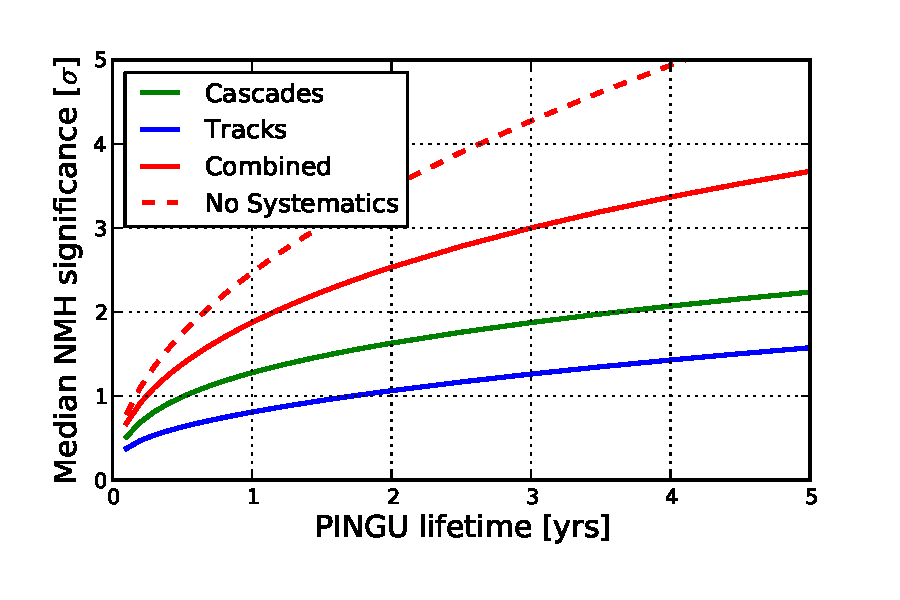
\includegraphics[width=0.495\linewidth]{sigma_vs_time_mDOM}}
  \subfloat[\label{fig:covmat_mDOM}]
   {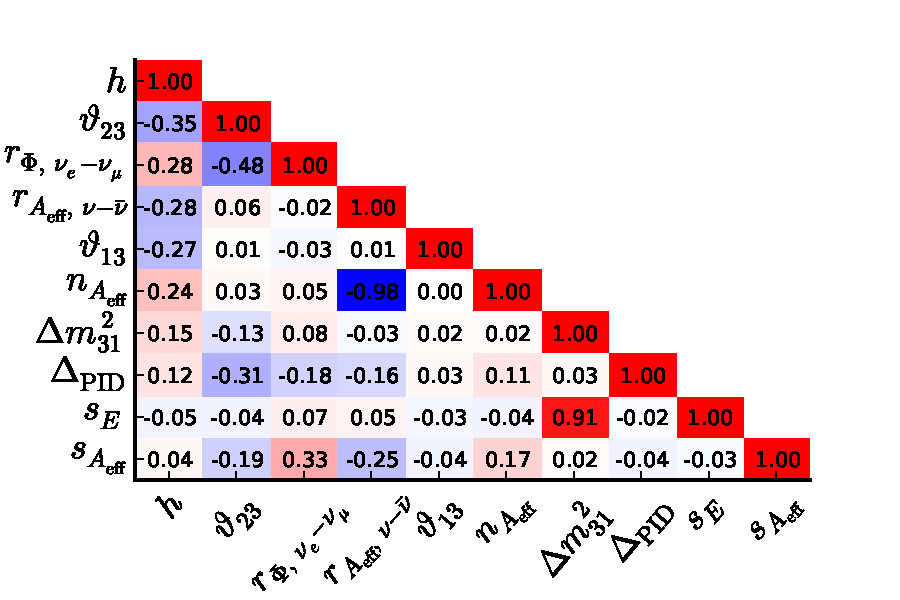
\includegraphics[width=0.495\linewidth]{CovMat_PINGU_mDOM}}
 \caption{\protect\subref{fig:sigma_vs_time_mDOM} Evolution of PINGU's expected
          mass hierarchy significance with time and
          \protect\subref{fig:covmat_mDOM} full correlation matrix for
          PINGU assuming reconstruction and particle identification as in
          geometry V15, \ie no module noise.}
 \label{fig:time_covmat_mDOM}
\end{figure}

\noindent
The segmented photosensitive area of the mDOM will allow for an almost perfect
rejection of noise hits. Thus the event signatures will be clearer, leading to
an improved reconstruction and particle identification. In \papa, this can be
modelled by using the parametrised reconstruction functions and event
classification extracted from the Monte Carlo data for geometry V15, which was
erroneously produced without simulating noise. As the difference to geometry
V36 in terms of module density---which is crucial for the reconstruction
performance---is rather small\footnote{Geometry V36 has a horizontal string
spacing of 22\,m and a vertical module spacing of 3\,m, while in V15 string and
module spacing are 20\,m and 5\,m, respectively.}, the resulting
parametrisations, written out in App.~\ref{app:reco_V15} and
\ref{app:PID_threechannel}, respectively, should give a good approximation of
what to expect for the baseline geometry V36 with fully suppressed noise.

The resulting significance as function of lifetime and the correlation matrix
are shown in Fig.~\ref{fig:time_covmat_mDOM}. Comparing this to the results for
the baseline settings in Fig.~\ref{fig:time_covmat}, only a very small
improvement can be observed. Looking at the correlation matrix, the most
obvious change is the increased impact of the mixing angle \thet{23} and the
flux ratio $r_{\Phi,\,\nue-\numu}$ on the mass hierarchy.

The reason for this
is that especially the cascade channel profits from the improved particle
identification, increasing its significance without systematics from
3.0\,$\sigma$ to 3.3\,$\sigma$\footnote{The full error listings are shown in
App.~\ref{app:fisher_mDOM}}, which is reflected by the increased significance
scale of the \delchi distribution in the cascade channel, shown in
Fig.~\ref{fig:akhmedov_mDOM}. As such a feature basically means more \nue-like
events being detected, it can of course be mimicked by a wrong relative
normalisation of the primary \nue and \numu fluxes or a stronger oscillation
from \numu to \nue, determined by the value of \thet{23}. Unfortunately, these
two parameters are insufficiently constrained by themselves, thus they can
partly ``absorb'' the gain in sensitivity to the mass hierarchy.

\begin{figure}[bhp]
 \centering
 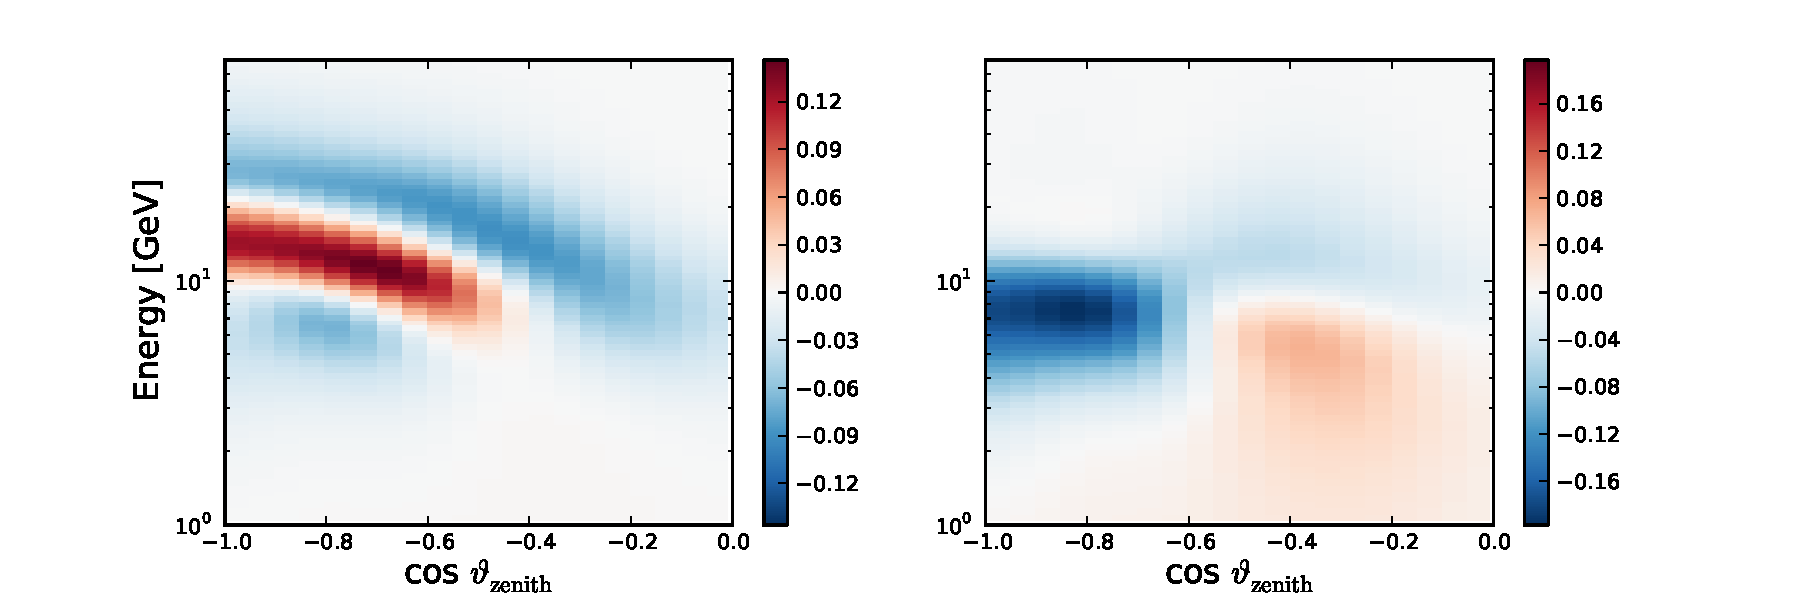
\includegraphics[width=\linewidth]{akhmedov_mDOM}
 \caption{\delchi distribution in the track (left) and cascade (right) channels
          assuming reconstruction and particle identification as in geometry
          V15, \ie no module noise.}
 \label{fig:akhmedov_mDOM}
\end{figure}


%==============================================================================
\section{Combining PINGU with JUNO}
\label{sec:JUNO}
%==============================================================================

\subsection{The JUNO Experiment}
\label{sec:JUNO_exp}

\begin{figure}[thp]
 \centering
 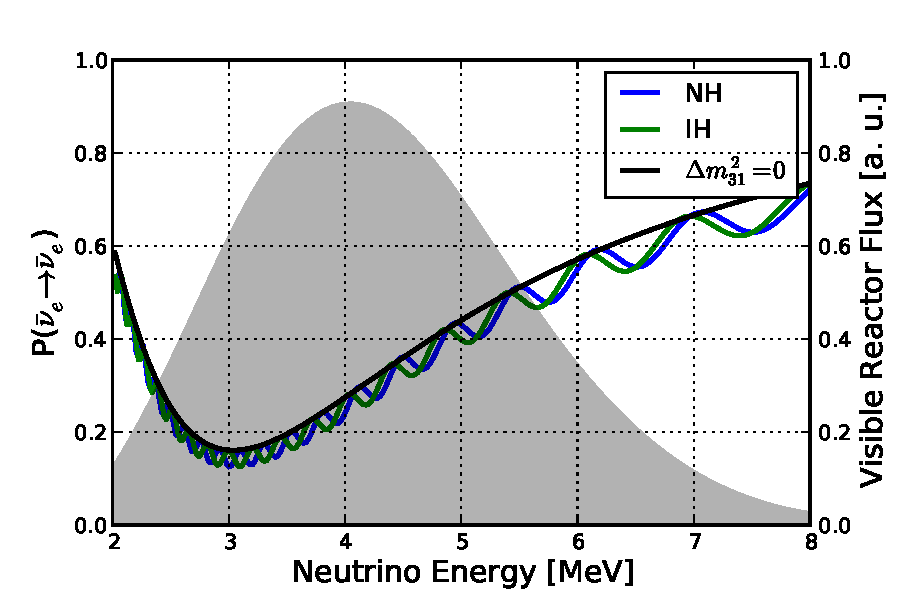
\includegraphics[width=0.7\linewidth]{JUNO_osc_probs}
 \caption{\nuebar survival probability for a baseline of 50\,km, overlaid with
  the un-oscillated nuclear reactor spectrum as it would be detected by JUNO
  (including detector acceptance).}
 \label{fig:JUNO_osc_probs}
\end{figure}

\noindent As already briefly discussed in Sec.~\ref{sec:ReacNuOsc}, 
JUNO\footnote{Short
for Jiangmen Underground Neutrino Observatory.} is a neutrino experiment under
construction in China's Guangdong Province. With its sensitive region at low MeV
energies, it is able to detect supernova and geoneutrinos, yet its main target
are reactor neutrinos from the Taishan and Yangjiang nuclear power plants to be
erected in $\approx 50$\,km distance each. These \nuebar's can be detected via
inverse beta decay:
\begin{equation}
 ^A_Z\mathrm{X} + \nuebar \quad \to\quad  ^A_{Z-1}\mathrm{Y} + e^+
\end{equation}

These \nuebar undergo oscillations that are mostly due to the smaller mass
splitting \dm{21}, but have a fast modulation due to \dm{31}. The vacuum \nuebar
survival probability\footnote{Matter effects can be neglected here.} can be
expressed analytically:
\begin{eqnarray}
 P(\nuebar\to\nuebar)\quad = \quad 1 &-& \cos^4(\thet{13})\,\sin^2(2\thet{12})\,
                            \sin^2\left(\dm{21}\frac{L}{4E}\right) \nonumber\\
                          &-& \cos^2(\thet{12})\, \sin^2(2\thet{13})\,
                            \sin^2\left(\dm{31}\frac{L}{4E}\right) \nonumber\\
                          &-& \sin^2(\thet{12})\, \sin^2(2\thet{13})\,
                            \sin^2\left(\dm{32}\frac{L}{4E}\right)
 \label{eqn:JUNO_osc_probs}
\end{eqnarray}
with $\dm{32} = \dm{31} - \dm{21}$. As shown in Fig.~\ref{fig:JUNO_osc_probs},
for a baseline of $L = 50$\,km this is dominated by the slow \dm{21}
oscillation, corresponding to the first term in (\ref{eqn:JUNO_osc_probs}). On
top of that is a pattern of rapid oscillation originating from the interference
of the second and third term of (\ref{eqn:JUNO_osc_probs}). The exact shape of
this pattern, especially the position of the local minima and maxima, depend on
the mass hierarchy which changes the relative sizes of \dm{31} and
\dm{32}\footnote{Their signs are irrelevant as the outer $\sin^2$ is symmetric
about zero.}.

\begin{figure}[thp]
 \centering
 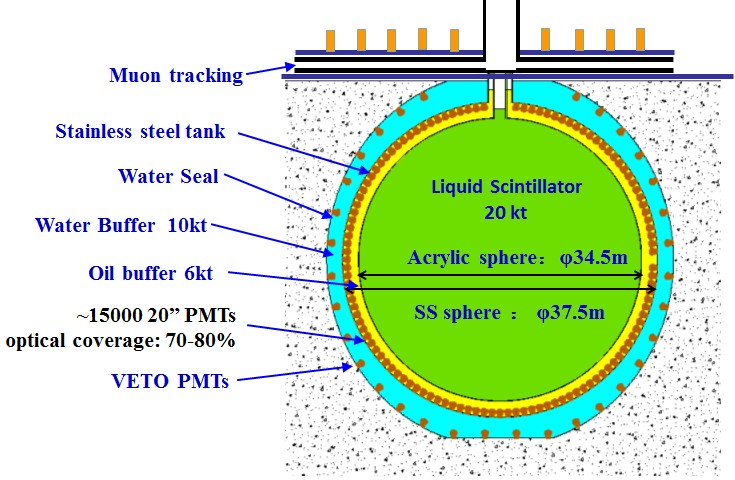
\includegraphics[width=0.7\linewidth]{JUNO}
 \caption{Layout of the JUNO detector. Figure taken from \cite{JUNO2}.}
 \label{fig:JUNO_layout}
\end{figure}

Taking the detector acceptance into account, the expected reactor neutrino
spectrum \cite{JUNO_TDR} is very suitable to observe this signal, as one can see
in Fig.~\ref{fig:JUNO_osc_probs} as well. However, a very precise energy
reconstruction is needed to actually resolve the spectral features associated
with the neutrino mass hierarchy.

With the detector setup shown in Fig.~\ref{fig:JUNO_layout}, a relative
resolution of $3\,\%/\sqrt{E [\mathrm{MeV}]}$ is aimed for. The target volume
is filled with 20\,kt of liquid scintillator to enhance the photon output. This
essentially destroys any directionality of the event signatures, however, no
information about the arrival direction of the neutrinos is needed as the
baseline for the oscillation is known\footnote{In PINGU, the \coszen
information is needed to infer the location where the neutrinos were generated
in the Earth's atmosphere and hence the distance they have travelled.}. The
inner surface of the volume is covered with $\approx 15000$ 20'' PMTs, resulting
in a photocoverage of at least 70\,\%. Tagging and vetoing of atmospheric muons
is ensured by scintillator tiles on top of the detector and a 10\,kt water
Cherenkov detector surrounding the target volume. Natural radioactivity is
buffered in a layer between muon veto and active region filled with 6\,kt of
mineral oil \cite{JUNO2}.

If this precision can indeed be realised, JUNO claims to be able to determine
the neutrino mass hierarchy with a significance of $\approx 3.3\,\sigma$ with a
total $10^5$ recorded neutrino events, corresponding to six years of data taking
\cite{JUNO, JUNO2, JUNO_TDR}. In the following sections a modification of \papa
is described, aiming at a detector simulation for JUNO instead of PINGU in order
to reproduce the reported sensitivity.

\subsection{Simulating JUNO with \papa}
\label{sec:JUNO_sim}

The major difference between the observable signals in PINGU and JUNO is that
PINGU will record a two-dimensional histogram in ($E$,\,\coszen) while in JUNO
only the energy spectrum is measured. Thus only one very narrow zenith bin
with edges at $\coszen = [-0.0039245,\,-0.0039235]$ is simulated, corresponding
to a baseline of 50\,km. In energy, 300 bins between 2\,MeV and 8\,MeV are
used. No oversampling is applied as the oscillation probabilities are
already sufficiently smooth (see Fig.~\ref{fig:JUNO_osc_probs}).

Since only the \nuebar survival probability is relevant for JUNO, which can be
calculated analytically according to (\ref{eqn:JUNO_osc_probs}), the
\texttt{PhysicsSimulation} has been extended by a module doing exactly this
analytical calculation. Avoiding the numerical solution of the Schr\"{o}dinger
equation, the \texttt{PhysicsSimulation} is sped up dramatically.

For the \texttt{DetectorSimulation}, the software itself is not changed,
however the inputs of course have to model the JUNO detector.
The neutrino flux is adopted from \cite{JUNO_TDR} and stored in a table of the
same format as the atmospheric flux tables provided by \cite{HondaSP}. This
flux, shown as an overlay in Fig.~\ref{fig:JUNO_osc_probs}, has the detector
acceptance already folded in, but is only given in arbitrary units. Thus, the
effective area is set to a constant value of 1\,m$^2$ for \nuebar CC and zero
for all other interaction channels while the analysis histograms will be
normalised to $10^5$ \nuebar events before analysis.

The directional reconstruction is parametrised by a single Gaussian with a
fixed width of $10^{-5}$ in \coszen, meaning that all events will stay in
place. As there is only one bin in \coszen, migration of events is impossible
in any case.

The energy reconstruction is represented by a single Gaussian as well, with
mean and width given by
\begin{eqnarray}
 \mu(E) &=& E - 0.8\,\mathrm{MeV} \\
 \sigma(E)/E &=& 4\,\%/\sqrt{E [\mathrm{MeV}] - 0.8} \quad.
\end{eqnarray}
The shift in energy reflects the fact that the visible energy in an inverse beta
decay is smaller than the initial neutrino energy. 511\,keV are needed to
create the $e^+$, which in turn stops to emit Cherenkov light once it falls
below the Cherenkov threshold (\ref{eqn:ChkovThr}), corresponding to a kinetic
energy of $\approx 280$\,keV depending on the optical medium. These two
contributions sum up to $\approx 0.8$\,MeV.
The relative energy resolution refers to the visible energy as well.
Additionally, it has been deteriorated \wrt the published specifications to be
$4\,\%/\sqrt{E_\mathrm{vis} [\mathrm{MeV}]}$. This reflects the fact that the
nuclear power plants used as neutrino sources have several reactor cores that
are up to 500\,m apart from each other. This introduces an uncertainty of 1\,\%
on the baseline $L$, which is equivalent to an additional uncertainty of 1\,\%
in the energy reconstruction as the relevant quantity is $L/E$.

\begin{figure}[thp]
 \centering
 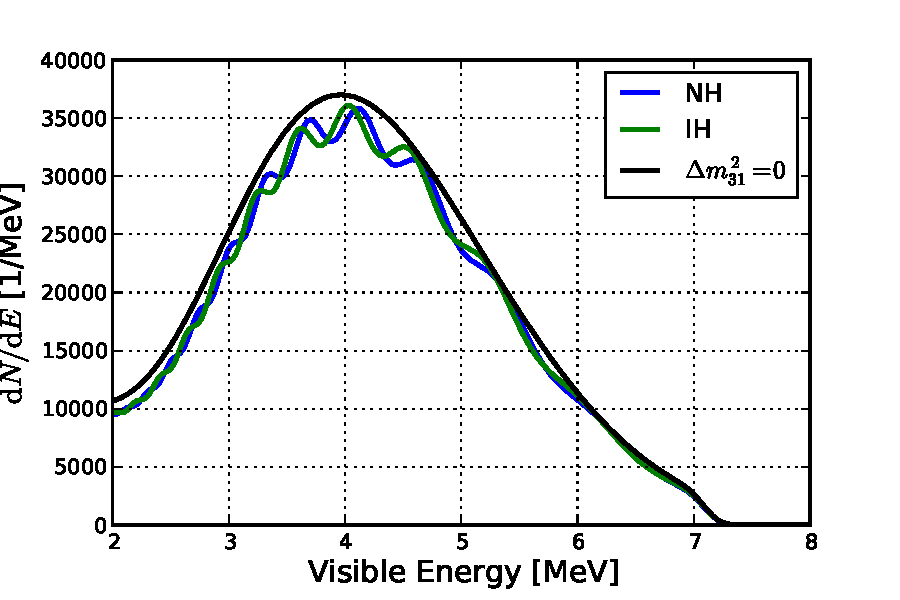
\includegraphics[width=0.7\linewidth]{JUNO_signal}
 \caption{Expected event spectrum in JUNO including all detector effects.}
 \label{fig:JUNO_signal}
\end{figure}

Finally, in JUNO there is no discrimination between cascade-like and track-like 
events as only \nuebar-induced inverse beta decays are expected. Hence, all 
events are classified as cascades and the track channel is not considered for 
the analysis. The resulting observed event distribution for the normal and 
inverted hierarchy case as well as for oscillations with $\dm{31} = 0$ is shown 
in Fig.~\ref{fig:JUNO_signal}.
\enlargethispage{\baselineskip}

\subsection{Preparing the JUNO Signal for Fisher Matrix Analysis}
\label{sec:JUNO_FFT}

\begin{figure}[thp]
 \centering
 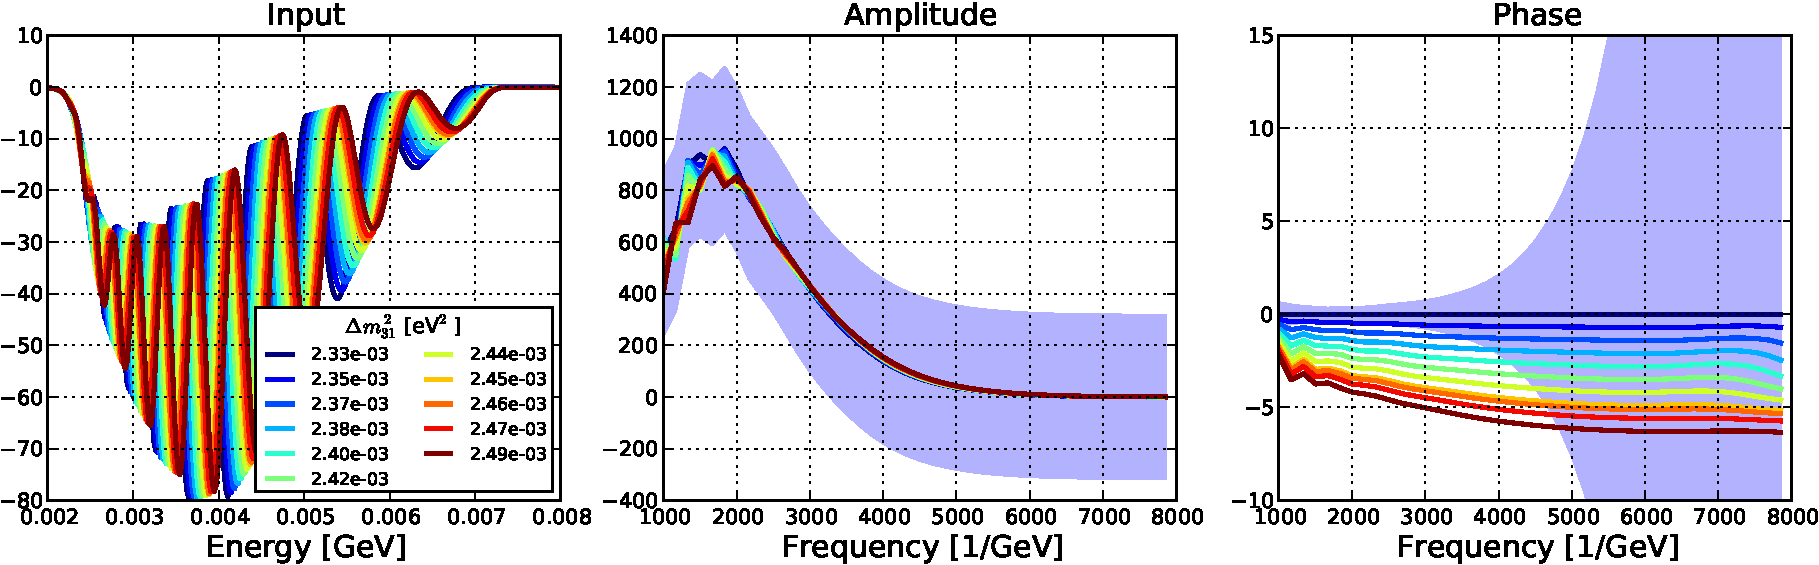
\includegraphics[width=\linewidth]{deltam31_FFT}
 \caption{Linearisation of the detector response to \dm{31} via Fourier 
  transformation. For details, refer to the text.}
 \label{fig:JUNO_FFT}
\end{figure}

\noindent In contrast to PINGU, the analysis histograms for JUNO as shown in 
Fig.~\ref{fig:JUNO_signal} cannot be used for the Fisher matrix analysis 
directly. The reason for this are the rapid oscillations of the event count as 
a function of energy that are the signal to be observed. This means that for a 
given bin in energy, the expected number of events is usually not a linear 
function of the systematic parameters. 
% This is true especially for \dm{31}, as 
% visible in the left panel of Fig.~\ref{fig:JUNO_FFT}. 
% Here, the expected signal 
% for $\dm{31}=0$ (black line in Fig.~\ref{fig:JUNO_signal}) has been subtracted 
% to show the features more clearly.

In order to apply the Fisher matrix formalism, JUNO's response to the 
systematic parameters has to be linearised. As the signal itself is 
oscillatory, the natural choice is to apply a Fourier transformation before 
analysis. To assure an input signal that smoothly fades out to zero at the 
edges of the considered energy interval, the expected signal for $\dm{31}=0$ 
(black line in Fig.~\ref{fig:JUNO_signal}) is subtracted from the actual event 
rates and an exponential cut-off at low energies applied to the result. 

This quantity is shown in the left panel of Fig.~\ref{fig:JUNO_FFT}, the 
non-linearity of the individual bin counts as a function of \dm{31} can clearly 
be seen. It is then fed to the implementation of the fast Fourier transform 
(FFT) algorithm \cite{FFT} provided by the \texttt{numpy} package.

As the input spectrum is real, only positive frequencies have to be considered
in the FFT result. In addition, frequencies below 1/MeV are ignored as they are
subject to large fluctuations. Thus the output of the FFT is a complex
frequency spectrum in the range from 1/MeV to 8/MeV, given as its real and
imaginary part. As the FFT is a linear transform, the error on both is given by
\begin{equation}
 \mathrm{FFT}(\Sigma) = \mathcal{F} \Sigma \mathcal{F}^H \quad,
 \label{eqn:FFTerror}
\end{equation}
where $\mathcal{F}$ is the Fourier matrix, \ie the Fourier transform of the
$n$-dimensional unit matrix where $n$ is the number of bins in the input
series, and $\mathcal{F}^H$ its conjugate transpose. $\Sigma$ is the
covariance matrix of the input data, see \eg \cite{FFT_Error1}.

In this case, the input data are independent bin counts $N_i$ with statistical
errors $\sigma_i = \sqrt{N_i}$, hence $\Sigma$ is diagonal:
\begin{equation}
 \Sigma = \mathrm{diag}(\vec{\sigma})
 = \mathrm{diag}(\sigma^2_1,\,\sigma^2_2,\,\dots,\,\sigma^2_n)
 = \mathrm{diag}(N_1,\,N_2,\,\dots,\,N_n)
\end{equation}
Propagating these properties through (\ref{eqn:FFTerror}) one finds that the
error on both the real and the imaginary part of the FFT output is constant and
proportional to the square root of the total number of bin
entries\footnote{The full error on any observable, \ie entry in the FFT output
spectrum, is given by the square root of the corresponding diagonal element of
the covariance matrix, cf.\ (\ref{eqn:sigma_full}).}:
\begin{equation}
 \Re[\mathrm{FFT}(\Sigma)] = \Im[\mathrm{FFT}(\Sigma)]
 = \mathlarger{\mathlarger{\mathbbm{1}}} \sum_{i=1}^n \sigma^2_i
 = \mathlarger{\mathlarger{\mathbbm{1}}} \sum_{i=1}^n N_i
 = \mathlarger{\mathlarger{\mathbbm{1}}} N_\mathrm{tot} 
\end{equation}

Yet for the analysis of the JUNO oscillation signal, amplitude and phase of the
complex spectrum are better suited than its real and imaginary part. These
quantities are calculated according to
\begin{eqnarray}
 A &=& \sqrt{\Re^2 + \Im^2} \\
 \phi &=& \arctan(\Im/\Re) + 2\pi k
\end{eqnarray}
with $k \in \mathbbm{N}$ assuring that $\phi$ increases monotonically with
increasing frequency, removing discontinuities. Their errors are then given by
\begin{eqnarray}
 \Delta A &=& \sqrt{\left(\frac{\Re}{A}\Delta\Re\right)^2
              + \left(\frac{\Im}{A}\Delta\Im\right)^2} =
              \sqrt{N_\mathrm{tot}}\\
 \Delta \phi &=& \Delta A / A \quad .
\end{eqnarray}

The FFT result in the amplitude-phase base is shown in the middle and right
panel of Fig.~\ref{fig:JUNO_FFT}.
One can see that the amplitude of the spectrum is virtually independent
from \dm{31} while the phase is approximately proportional to its
value\footnote{Note that all phases are shown relative to the phase spectrum
for $\dm{31}=2.33 \cdot 10^{-3}\,\mathrm{eV}^2$ to show the behaviour more
clearly.}. The shaded region marks the error range for the spectra for
$\dm{31}=2.33 \cdot 10^{-3}\,\mathrm{eV}^2$, for the other spectra the errors
are very similar.

\subsection{Results for JUNO}
\label{sec:JUNO_res}

\begin{table}[htpb]
 \caption{Uncertainties on all systematic parameters expected for JUNO with
  $10^5$ detected events, ranked according to their impact on the mass
  hierarchy parameter $h$.}
 \label{tab:JUNO_results}
 \begin{center}
  \small{\begin{tabular}{lrrrrrr} 
\toprule
Parameter & Impact [\%] & Best Fit & $\sigma^\mathrm{full}$ & $\sigma^\mathrm{stat}$ & $\sigma^\mathrm{syst}$ & Prior \\ 
\midrule
$h$ & 100.0 & \num{1.00e+00} & \num{3.32e-01} & \num{7.99e-02} & \num{3.22e-01} & free \\
$\vartheta_{13}$ [$^\circ$] & 54.9 & \num{8.93e+00} & \num{2.34e+00} & \num{5.62e-01} & \num{2.27e+00} & free \\
$\Delta m^2_{31}$ [eV$^2$] & 38.2 & \num{2.46e-03} & \num{1.71e-05} & \num{4.74e-06} & \num{1.64e-05} & free \\
$s_{A_\mathrm{eff},\,\mathrm{JUNO}}$ & 17.9 & \num{0.00e+00} & \num{8.26e+01} & \num{2.05e+01} & \num{8.00e+01} & free \\
$s_{E,\,\mathrm{JUNO}}$ & 15.0 & \num{1.00e+00} & \num{1.52e-02} & \num{5.14e-03} & \num{2.26e-02} & \num{2.00e-02} \\
$\vartheta_{12}$ & 10.5 & \num{3.36e+01} & \num{1.87e+00} & \num{8.65e-01} & \num{1.65e+00} & free \\
$\Delta m^2_{21}$ & 9.8 & \num{7.54e-05} & \num{6.96e-06} & \num{3.86e-06} & \num{5.79e-06} & free \\
$n_{A_\mathrm{eff},\,\mathrm{JUNO}}$ & 0.0 & \num{0.00e+00} & \num{2.00e-02} & \num{9.43e-02} & \num{2.79e+00} & \num{2.00e-02} \\
\bottomrule 
\end{tabular}
}
 \end{center}
\end{table}

\begin{figure}[thp]
 \centering
 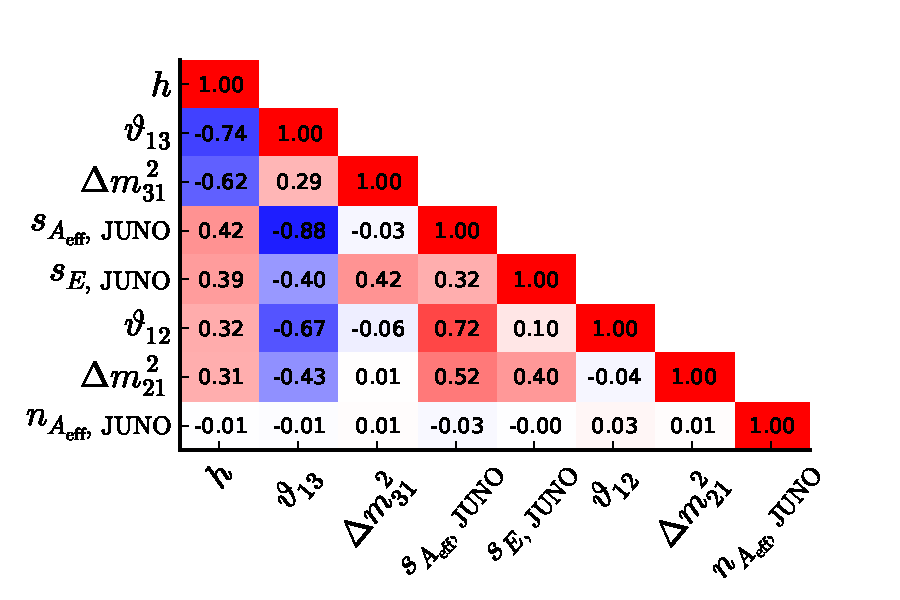
\includegraphics[width=0.7\linewidth]{CovMat_JUNO}
 \caption{Covariance matrix for JUNO, without external constraints on the
  oscillation parameters.}
 \label{fig:CovMat_JUNO}
\end{figure}

\noindent
Now that an observable has been constructed which is sufficiently linear as a
function of the parameters that JUNO will measure, the Fisher Matrix can be
applied.

The full error listing is given in Tab.~\ref{tab:JUNO_results}, where one can
read off a NMH sensitivity of $3.0\,\sigma$ for an event sample of
$N_\mathrm{tot} = 10^5$. Yet in contrast to the PINGU analysis, no priors have
been put on any of the oscillation parameters as the resulting significance is
to be compared to the one quoted by the JUNO collaboration themselves. In
\cite{JUNO2}, for a ``reactor-only analysis'', \ie no without external
knowledge, a confidence level of $\delchi^2 \approx 11$ is reported,
corresponding to a significance of $\mathcal{S} = \sqrt{\delchi^2} \approx
3.3\,\sigma$. This does not match up perfectly with the figure retrieved from
the modified \papa simulation, however the agreement is fairly good given that
the two calculations are completely independent in simulation and analysis
method, and in addition \papa was intended for a very different experiment.

Another claim from \cite{JUNO2} is that the NMH significance can be increased
to $\delchi^2 \approx 19\ \hat{=}\ \mathcal{S} \approx 4.4\,\sigma$ when using
a prior measurement of \dm{\mu\mu} with 1\,\% precision. This parameter can be
measured in \numu disappearance experiments, usually with a neutrino beam from
an accelerator travelling over a baseline of $\mathcal{O}$(100\,km). But since
\dm{\mu\mu} is a rather complex combination of all mixing parameters
\cite{Deltam_ee_mumu}, it is not possible to put the corresponding prior in the
base of mixing parameters chosen in this thesis.

One can, however, include priors on all mixing parameters according to a
current global fit \cite{Fogli} as it was done in the analysis for PINGU
(cf.\ Sec~\ref{sec:input_osc}). This increases the significance retrieved from
the Fisher Matrix to 4.6\,$\sigma$, a gain of 1.6\,$\sigma$ \wrt the value
without any priors. The full errors are listed in Tab.~\ref{tab:JUNO_priors}. In
JUNO's own analysis, only 1.1\,$\sigma$ are added by the inclusion of external
constraints, however there only one prior is put on an composite parameter,
which is a weaker statement than putting individual priors on four underlying
parameters.

The strongest impact on JUNO's expected sensitivity to the neutrino mass
hierarchy has the uncertainty of the mixing angle \thet{13}, as one can read
off from Tab.~\ref{tab:JUNO_results} and the covariance matrix, shown in
Fig.~\ref{fig:CovMat_JUNO}. Including the current knowledge of this parameter
alone enhances the significance to 4.4\,$\sigma$.

Next in size is the impact of \dm{31} on the mass hierarchy. For this parameter,
however, including the current knowledge as a prior does not significantly
improve the NMH measurement. The reason is that the current uncertainty on
\dm{31} is $8 \cdot 10^{-5}\,\mathrm{eV}^2$ \cite{Fogli}, while JUNO will
already provide a constraint of $1.7 \cdot 10^{-5}\,\mathrm{eV}^2$ by itself
(see Tab.~\ref{tab:JUNO_results}), \ie there is no other experiment that can
make a more precise measurement of \dm{31} than JUNO.

This sub-percent precision on the value of \dm{31} is stated by \cite{JUNO2},
too. A similar precision is claimed for \sinsq{\thet{12}} and \dm{21}. Looking
at Tab.~\ref{tab:JUNO_results}, however, the relative uncertainties from
the Fisher matrix are on the order of 10\,\%\footnote{For the relative error
on \sinsq{\thet{12}}, the errors listed in Tabs.~\ref{tab:JUNO_results} and
\ref{tab:JUNO_priors} for \thet{12} in degrees have to be converted:
$\sinsq{\thet{12}} \approx 0.306$ and
$\sigma^\mathrm{full}_{\sinsq{\thet{12}}}
= \frac{\partial \sinsq{\thet{12}}} {\partial \thet{12}}
  \sigma^\mathrm{full}_\thet{12}
= \sin(2\thet{12})\,\sigma^\mathrm{full}_\thet{12}$ with
$\sigma^\mathrm{full}_\thet{12}$ in radians.}. Yet in the given reference it
remains unclear whether the stated uncertainties include the prior on
\dm{\mu\mu}. After adding priors on all oscillation parameters, the
Fisher matrix still lists a precision of $\approx 3\,\%$ for both parameters
(see Tab.~\ref{tab:JUNO_priors}). 

\subsection{Joint Analysis of JUNO and PINGU}
\label{sec:JUNO_comb}

Finally, the results of PINGU and JUNO can be combined by adding the respective
Fisher matrices. To start off on common grounds, only the oscillation
parameters will be considered as systematics without any prior knowledge. This
severely decreases PINGU's NMH significance to only 1.5\,$\sigma$ after three
years of lifetime as it is strongly correlated with \thet{13}, see
Tab.~\ref{tab:PINGU_physonly}. Here a fundamental difference in the approaches
taken by PINGU and JUNO becomes evident: JUNO is able to determine the mass
hierarchy with appreciable significance all by itself, while in PINGU at least
the value of \thet{13} has to be retrieved from an independent experiment, \eg
Daya Bay \cite{DayaBay}. JUNO on the other hand still has a NMH significance of
3.5\,$\sigma$ considering only physics systematics without priors
(Tab.~\ref{tab:JUNO_physonly}).

\begin{table}[h!]
 \caption{Error listings for the combination of PINGU and JUNO, including only
  oscillation parameters without any priors.}
 \label{tab:combined_physonly}
 \begin{center}
  \smaller{\begin{tabular}{lrrrrrr} 
\toprule
Parameter & Impact [\%] & Best Fit & $\sigma^\mathrm{full}$ & $\sigma^\mathrm{stat}$ & $\sigma^\mathrm{syst}$ & Prior \\ 
\midrule
$h$ & 100.0 & \num{1.00e+00} & \num{2.33e-01} & \num{7.56e-02} & \num{2.21e-01} & free \\
$\Delta m^2_{31}$ [eV$^2$] & 83.4 & \num{2.46e-03} & \num{1.21e-05} & \num{4.58e-06} & \num{1.12e-05} & free \\
$\vartheta_{13}$ [$^\circ$] & 76.8 & \num{8.93e+00} & \num{1.01e+00} & \num{4.64e-01} & \num{8.99e-01} & free \\
$\vartheta_{12}$ & 2.5 & \num{3.36e+01} & \num{1.25e+00} & \num{8.65e-01} & \num{9.08e-01} & free \\
$\vartheta_{23}$ [$^\circ$] & 1.4 & \num{3.86e+01} & \num{3.05e-01} & \num{3.02e-01} & \num{3.79e-02} & free \\
$\Delta m^2_{21}$ & 0.7 & \num{7.54e-05} & \num{5.52e-06} & \num{3.86e-06} & \num{3.94e-06} & free \\
\bottomrule 
\end{tabular}
}
 \end{center}
\end{table}

If now the Fisher matrices of PINGU and JUNO are added, the combined
sensitivity to the NMH increases to 4.3\,$\sigma$, much larger than the square
sum of the individual sensitivities, which is 3.8\,$\sigma$. This is mainly due
to the good constraint on \thet{13} from JUNO being passed on to PINGU and
hence enhancing its NMH sensitivity. JUNO on the other hand can not profit much
from PINGU since the only parameter that it can measure with greater precision
than JUNO is \thet{23}, which does not affect JUNO at all.

A second outcome of the joint analysis is that JUNO's extremely precise
measurement of \dm{31} can be used to shrink down PINGU's error ellipse in
(\dm{31},\,\sinsq{\thet{23}}) parameter space, which was shown above in
Fig.~\ref{fig:AtmoParamsBaseline}. Fig.~\ref{fig:AtmoParamsWithJUNO} is an
update of the former including the expected result of JUNO. The combined
ellipse of PINGU and JUNO demonstrates the enormous improvement in the
knowledge about these two parameters that is to be expected over the course of
the next five to ten years---the time needed for the two experiments to be
constructed and take their nominal amount of data.

Since \dm{31} and \thet{23} are virtually uncorrelated in PINGU---as one can
recognise from the semi-major axes of PINGU's error ellipse that are
almost aligned to the coordinate axes---JUNO's strict constraint on \dm{31}
does not affect PINGU's precision on \thet{23}. Still the uncertainties on both
parameters will be reduced by almost one order of magnitude \wrt the current
precision.

\begin{figure}[thp]
 \centering
 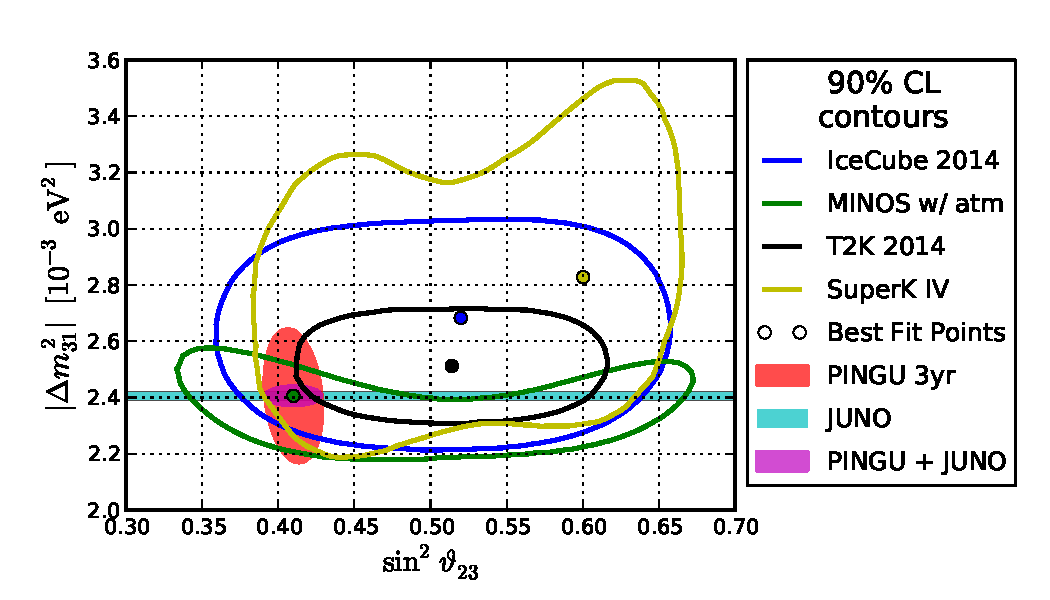
\includegraphics[width=0.85\linewidth]{AtmoParamsWithJUNO}
 \caption{Same as Fig.~\ref{fig:AtmoParamsBaseline}, adding JUNO's
  expected constraint on \dm{31} and the combined error ellipse of PINGU and
  JUNO.}
 \label{fig:AtmoParamsWithJUNO}
\end{figure}

\FloatBarrier

\section{Summary}
\label{sec:ana_summary}

In this chapter, PINGU's sensitivity to the neutrino oscillation parameters,
especially the neutrino mass hierarchy, has been studied in depth. The baseline
detector parametrisation leads to a median significance of 2.9\,$\sigma$ after
three years of data taking. Looking at the track and cascade channels
separately, the individual significances are 1.3\,$\sigma$ and 1.9\,$\sigma$,
respectively. This is a somewhat conservative estimate, and various effects
increasing the expected significance have been explored in this chapter. These
are summarised in Tab.~\ref{tab:sigma_summary}.

\begin{table}[t]
\caption{Summary of the effects studied in this chapter and their impact on
PINGU's sensitivity to the NMH, relative to the baseline settings.}
\label{tab:sigma_summary}

\begin{center}

\begin{tabularx}{\textwidth}{@{}YcccYc@{}}
\toprule
Model & Combined & Tracks & Cascades & Note & Section \\
\midrule
Baseline &
$2.9\,\sigma$ & $1.3\,\sigma$ & $1.9\,\sigma$ &
Absolute significance, reference for following rows &
\ref{sec:results_baseline} \\
Remove priors on oscillation parameters, no detector nuisance parameters & 
$-1.4\,\sigma$ & $-1.0\,\sigma$ & $-0.6\,\sigma$ &
To be compatible with JUNO's own analysis &
\ref{sec:JUNO_comb} \\
\midrule
\thet{23} in 2nd octant&
$+2.7\,\sigma$ & $+0.2\,\sigma$ & $+2.3\,\sigma$ &
Fiducial value of \thet{23} mirrored at $45^\circ$ &
\ref{sec:results_octant} \\
True normal NMH &
$+0.2\,\sigma$ & $+0.0\,\sigma$ & $+0.2\,\sigma$ & 
& 
\ref{sec:results_NHtrue} \\
\midrule
Three-channel PID &
$+0.2\,\sigma$ & $\pm0.0\,\sigma$ & $-0.4\,\sigma$ &
Unidentified events contribute $1.3\,\sigma$ \hspace{3cm}
Reference uses PID from geometry V15  & 
\ref{sec:results_includeunkn} \\
No module noise & 
$+0.1\,\sigma$ & $+0.0\,\sigma$ & $+0.0\,\sigma$ & 
PINGU built from mDOMs &
\ref{sec:mdom_effect} \\
Photon statistics doubled & 
$+0.9\,\sigma$ & $+0.9\,\sigma$ & $+0.8\,\sigma$ &
PINGU built from WOMs &
\ref{sec:wom_effect} \\
\midrule
Combining with JUNO &
$+2.8\,\sigma$ & n/a & n/a &
JUNO contributes $3.5\,\sigma$ \hspace{3cm}
Reference is second row & 
\ref{sec:JUNO_comb} \\
\bottomrule
\end{tabularx}

\end{center}

\end{table} 

The choice of the fiducial values for the oscillation parameters puts PINGU's 
baseline sensitivity to the neutrino mass hierarchy at the lower bound of the 
range of possible values: As one can see from the second set of rows in 
Tab.~\ref{tab:sigma_summary}, PINGU will determine the NMH with higher 
significance if the true mass hierarchy is normal or \thet{23} is in the second 
octant. The latter effect is much more dramatic, possibly almost doubling the 
expected significance. In both cases, the increase is primarily due to the 
cascade channel.

Technical improvements to the detector itself are covered in the third section 
of the table. A more evolved event classification with more channels than just 
tracks and cascades only leads to a moderate increase of the NMH sensitivity, 
thus efforts to modify the PID in this direction seem not too promising. In 
terms of sensor technology, a further reduction of the module noise has 
virtually no positive impact on the significance. This points to the conclusion 
that already with current optical modules random noise does not notably affect 
the event reconstruction---the noise cleaning algorithms 
(Sec.~\ref{sec:reco_noise}) are very effective and the reconstruction results 
stable against small perturbations. Increasing the number of detected photons 
per neutrino energy by enhancing the photosensitive area per sensor on the 
other hand leads to improved reconstruction results. From these, PINGU's NMH 
measurement can indeed profit, as the features of the mass hierarchy pattern 
can be resolved more precisely.

The last section of Tab.~\ref{tab:sigma_summary} covers the combination of
PINGU and JUNO. For this, all priors and detector parameters are removed,
strongly reducing PINGU's sensitivity, especially in the track channel. The
joint analysis with JUNO then leads to an expected NMH significance exceeding
all values before, however the signal is mostly driven by JUNO.

Through all the analyses the picture holds that the cascade channel is driving
PINGU's sensitivity to the neutrino mass hierarchy. Not only is its intrinsic
significance higher than the track channel's, it also contributes most of the
possible enhancement due to varying fiducial settings of the oscillation
parameters and refined particle identification. In addition it is more stable
if external constraints are loosened---the track channel on the other hand
loses its discrimination power almost completely in this case.

%==============================================================================
\chapter{Conclusion}
\label{sec:conclusion}
%==============================================================================

In this thesis, the development of \papa, a standalone simulation for the
planned PINGU atmospheric neutrino experiment, has been described. With \papa,
the expected event histograms in ($E$,\,\coszen) can be generated directly from
inputs like the atmospheric neutrino flux, oscillation probabilities, effective 
areas of the detector
and a parametrisation of the detector resolution, taking into account a variety
of systematic parameters, cf.\ Sec.~\ref{sec:papa}. Since most of the inputs are
extracted from Monte Carlo data in advance, the time-consuming event-by-event
simulation can be avoided in \papa, making it well suited to explore PINGU's
multi-dimensional parameter space in short time and robustly even in case of
rather low Monte Carlo statistics.

Using the results of \papa, PINGU's capability to measure the oscillation
parameters \thet{23} and \dm{31} and especially to determine the neutrino mass
hierarchy, \ie the sign of \dm{31}, was assessed with the Fisher matrix
technique. This analysis method, whose application to a particle physics
experiment is novel, is especially suited for problems with a large number of
parameters and essentially linear detector response to these parameters.

After checking that the requirements for applying the Fisher matrix are met
(Sec.~\ref{sec:fisher_prereq}), PINGU's performance was evaluated for its
current baseline geometry V36 with the most up-to-date estimates of
reconstruction resolution. In Sec.~\ref{sec:results_baseline} it was shown
that for a nominal lifetime of three years, PINGU is expected to determine the
neutrino mass hierarchy with a confidence level of 2.9\,$\sigma$, with the major
contribution coming from the analysis of cascade-like events\footnote{All events
that are not caused by a \numu or \numubar CC interaction, \ie without an
outgoing muon.}. In addition, PINGU will provide precision measurements of the
oscillation parameters \dm{31} and \thet{23}, and in particular resolve the
octant of \thet{23}. The latter is possible as PINGU observes neutrino
oscillations in matter, where the symmetry between the two octants is broken.
This also means that the asymmetry between the normal and inverted mass
hierarchy cases grows with an increasing value of \thet{23}, such that the
expected significance of the mass hierarchy measurement can reach 5\,$\sigma$
and more if the true value of \thet{23} is in the second octant.
The use of next-generation optical sensors---like the WOM concept, for which
basic work has been done in the context of this thesis---can further enhance
PINGU's performance by increasing the expected photon statistics per event and
hence improving the detection threshold and reconstruction precision
(Sec.~\ref{sec:om_effects}).

Finally, in Sec.~\ref{sec:JUNO} a combined analysis of PINGU and JUNO, a medium
baseline reactor neutrino experiment currently under construction, was done to
explore possible synergies. Given the respective settings, JUNO's expected
neutrino spectrum could be simulated with \papa without any modifications. Yet
for the analysis with the Fisher matrix method the spectrum had to be Fourier
transformed to achieve linear relations between the observables and the 
underlying physical
parameters. After this, JUNO's sensitivity to the neutrino mass hierarchy as
reported by the JUNO collaboration itself could be reproduced. The combined
analysis of both experiments, \ie adding the respective Fisher matrices,
results in a NMH significance exceeding the squared sum of the individual ones
by 0.5\,$\sigma$, mainly due to PINGU profiting from JUNO's constraint on the
oscillation parameter \thet{13}\footnote{For this study, no detector systematics
were considered and no external constraints were put on the oscillation
parameters.}.

In a broader picture, intermediate results of this work have been published as
official sensitivity estimates by the PINGU collaboration. The current version
of the PINGU Letter of Intent \cite{LoI} relies on the \papa simulation of the
previous baseline geometry V15, evaluated with the Fisher matrix technique. An
update of this report is planned in the near future, referring to the
current baseline geometry V36, reflecting all improvements on event
selection, reconstruction etc.\ achieved in the meantime, and covering a wider
range of systematic parameters.

In this update, the analysis will only partly depend on \papa. The main
calculations will be done with \texttt{pisa} \cite{pisa}, the software framework
\papa has evolved into. It keeps the idea of a direct simulation of event
histograms in a staged way and develops it further. Separating the individual
stages even more than \papa, \texttt{pisa} offers the option to add alternative
implementations of particular stages\footnote{E.\,g.\ other oscillation codes,
event reconstruction from parametrised reconstruction functions or directly
from Monte Carlo data, \dots} and easily apply different analysis
methods\footnote{E.\,g.\ the Fisher Matrix and the Likelihood Ratio techniques.}
to exactly the same data, as well as better maintainability of the code itself.

Since \papa and the Fisher Matrix analysis have been fully re-implemented
within \texttt{pisa} and both input and output format are compatible, the
results presented in this thesis can always be reproduced. Vice versa, the
concepts first introduced here, namely the staged simulation of event
histograms using parametrisations fitted to distributions of Monte Carlo events
and the Fisher matrix analysis, leading to a very fast evaluation of systematic
effects, will stay present within PINGU and might even be adopted by other
collaborations.

%------------------------------------------------------------------------------
\appendix
% \part*{Appendix}
%
% Add your appendices here - don't forget to also add them
% to \includeonly above
\chapter{Applicability of the Fisher Matrix}
\label{app:fisher_valid}

As established in Sec.~\ref{sec:fisher_prereq}, one requirement for the Fisher
Matrix to be valid is that the observables (\ie the bin counts for PINGU) are
described by linear functions of the parameters, hence the partial derivatives
entering (\ref{eqn:fisher_def}) can be considered to be constant within the
considered range. To quantify the non-linearity, one can define the quantity
\begin{equation}
 \Upsilon_n(p_i) = \left(N_n(p_{i,\,\mathrm{fid}} + \sigma_{p_i}) -
                          N_n(p_{i,\,\mathrm{fid}}) +
                     \frac{\partial N_n}{\partial p_i}\sigma_{p_i}\right)
                       \bigg/ N_n(p_{i,\,\mathrm{fid}}) \quad,
 \label{eqn:non-lin}
\end{equation}
describing the relative contribution of the non-linear terms to the variation
of the event count $N_b$ in bin $b$ as a function of the parameter $p_i$ over
its uncertainty range $p_{i,\,\mathrm{fid}} \pm \sigma_{p_i}$.

As one can see from Figs.~\ref{fig:nonlinearities1} and
\ref{fig:nonlinearities2}, for the simple scaling parameters like the mass
hierarchy $h$ or the overall normalisation $n_\aeff$ non-linearities are on the
order of the machine precision. But also for the physics parameters they are
typically smaller than $10^{-3}$, hence the requirement of linearity is well
fulfilled.

For means of illustration, the actual dependence of all bin entries on the
systematic parameters is shown as well. By eye, deviations from linearity can
only be recognised for \dm{31} and the energy scale. Since both shift the
sinusoidal oscillation pattern in energy non-linearities have to be expected,
however they only occur on a scale conceivably larger than the actual
uncertainty range.

\begin{figure}[p]
 \centering
 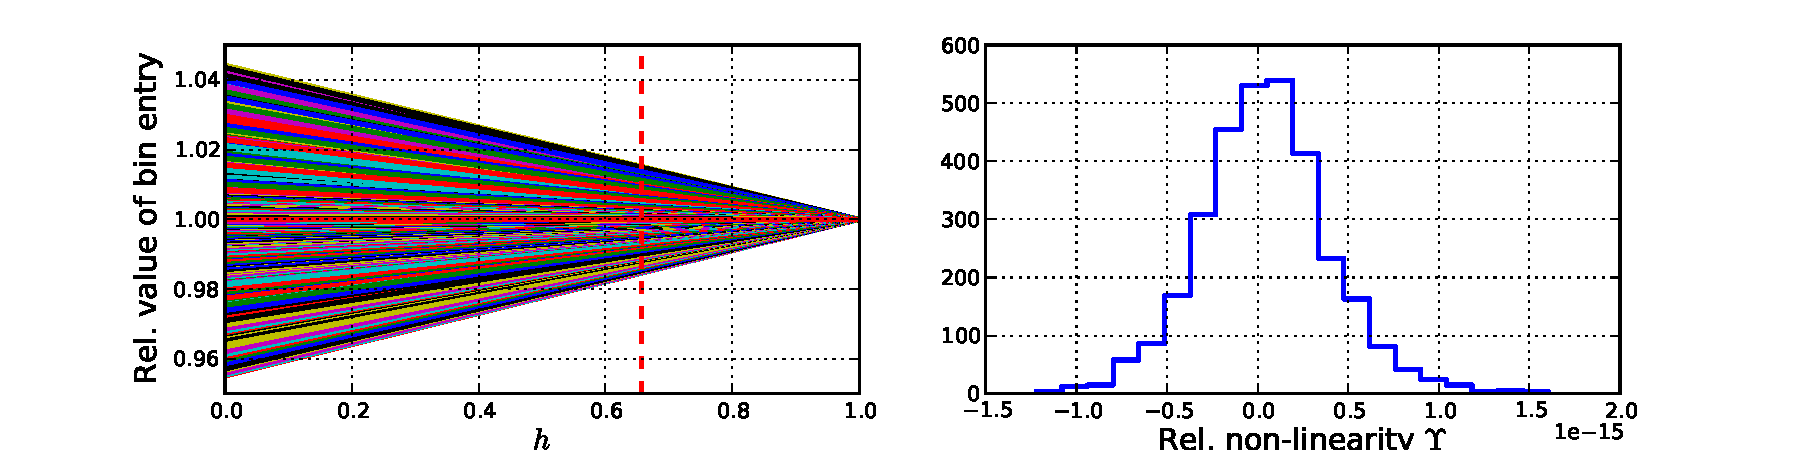
\includegraphics[width=\linewidth]{hierarchy}
 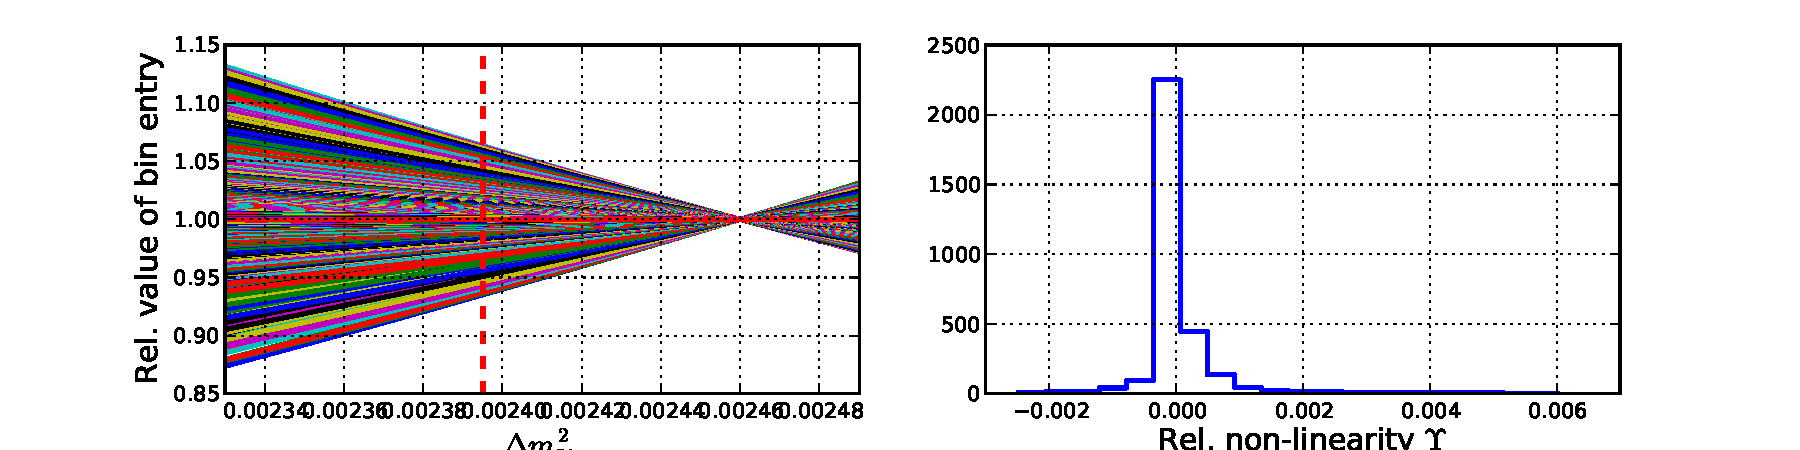
\includegraphics[width=\linewidth]{deltam31}
 \includegraphics[width=\linewidth]{theta23}
 \includegraphics[width=\linewidth]{theta13}
 \includegraphics[width=\linewidth]{energy_scale}
 \caption{\emph{Left:} Relative values of all bin entries in the analysis
  histograms as functions of the systematic parameters. The the entries at the 
  fiducial parameter values are set to one. The vertical lines indicate the full
  error range as listed in Tab.~\ref{tab:baseline_results}. \\
  \emph{Right:} Histograms of the non-linearities $\Upsilon$ of the bin counts
  as functions of different systematic parameters (see equation
  (\ref{eqn:non-lin})).}
 \label{fig:nonlinearities1}
\end{figure}

\begin{figure}[p]
 \centering
 \includegraphics[width=\linewidth]{a_eff_scale_flat}
 \includegraphics[width=\linewidth]{nu_rel_xsec_scale}
 \includegraphics[width=\linewidth]{nue_numu_flux_scale}
 \includegraphics[width=\linewidth]{a_eff_scale}
 \includegraphics[width=\linewidth]{PID_offset}
 \caption{Same as Fig.~\ref{fig:nonlinearities1} for the remaining parameters.}
 \label{fig:nonlinearities2}
\end{figure}


\chapter{Oscillation Probabilities}
\label{app:oscillation}

\section*{\refstepcounter{section}\thesection\quad Baseline Settings}

\begin{figure}[h]
 \centering
 \includegraphics[width=0.95\textwidth]{osc_ds_nue_to_nue}
 \caption{Oscillation probabilities for $\nue \to \nue$ (top) and $\nuebar \to
          \nuebar$ (bottom) for normal and inverted hierarchy.}
\end{figure}


\begin{figure}[t!]
 \centering
 \includegraphics[width=0.95\textwidth]{osc_ds_nue_to_numu}
 \caption{Oscillation probabilities for $\nue \to \numu$ (top) and $\nuebar \to
          \numubar$ (bottom) for normal and inverted hierarchy.}
\end{figure}

\begin{figure}[b!]
 \centering
 \includegraphics[width=0.95\textwidth]{osc_ds_nue_to_nutau}
 \caption{Oscillation probabilities for $\nue \to \nutau$ (top) and $\nuebar \to
          \nutaubar$ (bottom) for normal and inverted hierarchy.}
\end{figure}

\begin{figure}[t!]
 \centering
 \includegraphics[width=0.95\textwidth]{osc_ds_numu_to_nue}
 \caption{Oscillation probabilities for $\numu \to \nue$ (top) and $\numubar \to
          \nuebar$ (bottom) for normal and inverted hierarchy.}
\end{figure}

\begin{figure}[b!]
 \centering
 \includegraphics[width=0.95\textwidth]{osc_ds_numu_to_numu}
 \caption{Oscillation probabilities for $\numu \to \numu$ (top) and $\numubar
          \to \numubar$ (bottom) for normal and inverted hierarchy.}
\end{figure}


\begin{figure}[t!]
 \centering
 \includegraphics[width=0.95\textwidth]{osc_ds_numu_to_nutau}
 \caption{Oscillation probabilities for $\numu \to \nutau$ (top) and $\numubar
          \to \nutaubar$ (bottom) for normal and inverted hierarchy.}
\end{figure}

\clearpage
\section*{\refstepcounter{section}\thesection\quad Scanning the fiducial value
of \thet{23}}

\begin{figure}[b!]
 \centering
 \includegraphics[width=0.9\linewidth]{P_NH_and_diff_numu_to_nue_th23_41deg}
 \includegraphics[width=0.9\linewidth]{P_NH_and_diff_numu_to_nue_th23_45deg}
 \includegraphics[width=0.9\linewidth]{P_NH_and_diff_numu_to_nue_th23_48deg}
 \includegraphics[width=0.9\linewidth]{P_NH_and_diff_numu_to_nue_th23_51deg}
 \caption{Probabilities for $\numu\to\nue$ oscillations in normal mass
  hierarchy (left column) and difference between normal and inverted hierarchy
  oscillation probabilities (right column) for different values of \thet{23} in
  both octants.}
 \label{fig:osc_probs_scan_th23}
\end{figure}


\chapter{Parametrisations of the Detector Resolutions}
\label{app:reco_params}

The full parametrisations of the reconstruction performances will be listed in
form of the actual \papa input. These are nested dictionaries giving the
resolutions in energy (\texttt{'e'}) and \coszen (\texttt{'coszen'}) for all
four interaction channels: \nue, \numu, and \nutau CC (\texttt{'nue'},
\texttt{'numu'}, and \texttt{'nutau'}, respectively) and \nux NC
(\texttt{'NC'}). For each of those the resolution is given by the five
parameters \texttt{'fraction'}, \texttt{'loc1'}, \texttt{'loc2'},
\texttt{'width1'}, and \texttt{'width2'}, corresponding to $f$, $\mu_1$,
$\mu_2$, $\sigma_1$ and $\sigma_2$ in (\ref{eqn:reco_param}).

The actual function definitions for the five parameters is then supplied as a
text string that can be interpreted as a python function by python's
\texttt{eval()} function. In those definitions, \texttt{'n'} is a shorthand
for the numpy library \cite{numpy} used for most of the numerical operations in
\papa.

\section*{\refstepcounter{section}\thesection\quad Baseline Settings}

\small{\VerbatimInput{figs/reco_param/reco_default.json}}

\section*{\refstepcounter{section}\label{app:reco_V15}\thesection\quad Geometry
V15 (Noiseless)}

\small{\VerbatimInput{figs/reco_param/reco_V15.json}}

\chapter{PID Functions}
\label{app:pid}

\section*{\refstepcounter{section}\thesection\quad Baseline Settings}

The particle identification is a binary decision, thus only the track
identification probabilities $P_{\mathrm{channel} \to \mathrm{track}}$ are
listed:
\begin{eqnarray}
 P_{\nue\to\mathrm{track}}(E) &=&
   0.192 \gauss{\log_{10}(E[\mathrm{GeV}])}{0.878}{0.404} + 0.0309 \\
 P_{\numu\to\mathrm{track}}(E) &=&
   \frac{0.687}{\stepfunc{\log_{10}(E[\mathrm{GeV}])}{0.683}{0.183}} + 0.0585 \\
 P_{\nutau\to\mathrm{track}}(E) &=&
   0.197 \gauss{\log_{10}(E[\mathrm{GeV}])}{1.28}{0.466} + 0.0732 \\
 P_{\nux\,\mathrm{NC}\to\mathrm{track}}(E) &=&
   0.171 \gauss{\log_{10}(E[\mathrm{GeV}])}{1.37}{0.483} + 0.0339
\end{eqnarray}
The cascade identification probabilities are given by $P_{\mathrm{channel} \to
\mathrm{cascade}} = 1 - P_{\mathrm{channel} \to \mathrm{track}}$.

\section*{\refstepcounter{section}\label{app:PID_threechannel}\thesection\quad 
High-Purity Event Classification}

\begin{figure}[h!]
 \centering
 \includegraphics[width=0.495\linewidth]{PID_V15_trck}
 \includegraphics[width=0.495\linewidth]{PID_V15_cscd}
 \caption{Classification efficiencies for the high-purity track (left) and
          cascade (right) selections for PINGU V15, similar to
          Fig.~\ref{fig:PID}.}
 \label{fig:PID_threechannel}
\end{figure}

The particle identification is done by selecting high-purity track and cascade
samples, events ending up in neither sample are classified as ``unidentified'':
\begin{eqnarray}
 P_{\nue\to\mathrm{track}}(E) &=&
   0.0481 \gauss{\log_{10}(E[\mathrm{GeV}])}{0.904}{0.265} + 0.0350 \\
 P_{\nue\to\mathrm{cascade}}(E) &=&
   \frac{0.945}{\stepfunc{\log_{10}(E[\mathrm{GeV}])}{0.922}{0.180}} + 0.0264 \\
 P_{\numu\to\mathrm{track}}(E) &=&
   \frac{0.782}{\stepfunc{\log_{10}(E[\mathrm{GeV}])}{0.808}{0.135}} + 0.0507 \\
 P_{\numu\to\mathrm{cascade}}(E) &=&
   \frac{0.103}{\stepfunc{\log_{10}(E[\mathrm{GeV}])}{0.499}{0.127}} + 0.0223 \\
 P_{\nutau\to\mathrm{track}}(E) &=&
   \frac{0.125}{\stepfunc{\log_{10}(E[\mathrm{GeV}])}{0.882}{0.120}} + 0.0396 \\
 P_{\nutau\to\mathrm{cascade}}(E) &=&
   \frac{0.811}{\stepfunc{\log_{10}(E[\mathrm{GeV}])}{1.19}{0.200}} + 0.0163 \\
 P_{\nux\,\mathrm{NC}\to\mathrm{track}}(E) &=&
   \frac{0.0344}{\stepfunc{\log_{10}(E[\mathrm{GeV}])}{0.939}{0.0516}} + 0.0439
\\
 P_{\nux\,\mathrm{NC}\to\mathrm{cascade}}(E) &=&
   \frac{0.771}{\stepfunc{\log_{10}(E[\mathrm{GeV}])}{1.34}{0.216}} + 0.0202 
\end{eqnarray}
The fit of these functions to data is shown in Fig.~\ref{fig:PID_threechannel}.


\chapter{Full Error Listings}
\label{app:fisher_output}

Here the full error lists, similar to Tab.~\ref{tab:baseline_results}, for
various detector settings and sub-channels will be collected. These have
not been included in the main text for the sake of better readability. For a
description how to read the tables, refer to the explanations given for
Tab.~\ref{tab:baseline_results} in Sec.~\ref{sec:results_baseline}.

\section*{\refstepcounter{section}\label{app:fisher_baseline}\thesection\quad
Baseline Settings}

\begin{table}[h!]
 \caption{Same as Tab.~\ref{tab:baseline_results}, but for the track channel
  only}
 \begin{center}
  \small{\begin{tabular}{lrrrrrr} 
\toprule
Parameter & Impact [\%] & Best Fit & $\sigma^\mathrm{full}$ & $\sigma^\mathrm{stat}$ & $\sigma^\mathrm{syst}$ & Prior \\ 
\midrule
$h$ & 100.0 & \num{1.00e+00} & \num{7.47e-01} & \num{3.20e-01} & \num{6.75e-01} & free \\
$s_E$ & 8.4 & \num{1.00e+00} & \num{2.98e-02} & \num{8.36e-03} & \num{3.62e-02} & \num{5.00e-02} \\
$\Delta m^2_{31}$ [eV$^2$] & 7.2 & \num{2.46e-03} & \num{6.70e-05} & \num{1.93e-05} & \num{1.21e-04} & \num{8.00e-05} \\
$\vartheta_{23}$ [$^\circ$] & 5.9 & \num{3.86e+01} & \num{5.83e-01} & \num{3.55e-01} & \num{5.44e-01} & \num{1.32e+00} \\
$\vartheta_{13}$ [$^\circ$] & 3.6 & \num{8.93e+00} & \num{4.67e-01} & \num{9.47e-01} & \num{1.01e+01} & \num{4.68e-01} \\
$r_{\Phi,\,\nu_e-\nu_\mu}$ & 2.4 & \num{0.00e+00} & \num{3.61e-02} & \num{5.84e-03} & \num{5.17e-02} & \num{5.00e-02} \\
$\Delta_\mathrm{PID}$ [GeV] & 2.3 & \num{0.00e+00} & \num{3.82e-02} & \num{1.71e-02} & \num{3.43e-02} & \num{5.00e-01} \\
$s_\mathrm{PID}$ & 1.3 & \num{1.00e+00} & \num{3.04e-02} & \num{3.87e-03} & \num{3.01e-02} & free \\
$s_{A_\mathrm{eff}}$ [m$^2$/GeV] & 0.3 & \num{0.00e+00} & \num{4.13e-04} & \num{1.64e-04} & \num{3.79e-04} & free \\
$r_{A_\mathrm{eff},\,\nu-\bar\nu}$ & 0.2 & \num{0.00e+00} & \num{4.88e-02} & \num{9.29e-03} & \num{2.22e-01} & \num{5.00e-02} \\
\bottomrule 
\end{tabular}
}
 \end{center}
\end{table}

\begin{table}[h!]
 \caption{Same as Tab.~\ref{tab:baseline_results}, but for the cascade channel
  only}
 \begin{center}
  \small{\begin{tabular}{lrrrrrr} 
\toprule
Parameter & Impact [\%] & Best Fit & $\sigma^\mathrm{full}$ & $\sigma^\mathrm{stat}$ & $\sigma^\mathrm{syst}$ & Prior \\ 
\midrule
$h$ & 100.0 & \num{1.00e+00} & \num{5.17e-01} & \num{3.39e-01} & \num{3.91e-01} & free \\
$r_{\Phi,\,\nu_e-\nu_\mu}$ & 24.9 & \num{0.00e+00} & \num{2.44e-02} & \num{1.06e-02} & \num{2.58e-02} & \num{5.00e-02} \\
$\vartheta_{23}$ [$^\circ$] & 20.7 & \num{3.86e+01} & \num{1.05e+00} & \num{5.78e-01} & \num{1.61e+00} & \num{1.32e+00} \\
$\Delta_\mathrm{PID}$ [GeV] & 11.4 & \num{0.00e+00} & \num{1.53e-01} & \num{4.14e-02} & \num{1.55e-01} & \num{5.00e-01} \\
$s_{A_\mathrm{eff}}$ [m$^2$/GeV] & 4.5 & \num{0.00e+00} & \num{3.96e-04} & \num{1.85e-04} & \num{3.50e-04} & free \\
$r_{A_\mathrm{eff},\,\nu-\bar\nu}$ & 4.2 & \num{0.00e+00} & \num{4.91e-02} & \num{5.55e-03} & \num{2.60e-01} & \num{5.00e-02} \\
$\vartheta_{13}$ [$^\circ$] & 3.0 & \num{8.93e+00} & \num{4.66e-01} & \num{1.67e+00} & \num{5.53e+00} & \num{4.68e-01} \\
$s_E$ & 1.5 & \num{1.00e+00} & \num{3.14e-02} & \num{1.92e-02} & \num{3.55e-02} & \num{5.00e-02} \\
$\Delta m^2_{31}$ [eV$^2$] & 1.2 & \num{2.46e-03} & \num{6.73e-05} & \num{4.44e-05} & \num{1.16e-04} & \num{8.00e-05} \\
$n_{A_\mathrm{eff}}$ & 0.1 & \num{0.00e+00} & \num{2.29e-02} & \num{2.32e-03} & \num{2.29e-02} & \num{2.00e-01} \\
\bottomrule 
\end{tabular}
}
 \end{center}
\end{table}

\clearpage
\section*{\refstepcounter{section}\label{app:fisher_threechannel}
\thesection\quad High-Purity Event Classification}

\begin{table}[h!]
 \caption{Full error listings for the high-purity track channel, see
Sec.~\ref{sec:results_includeunkn}.}
 \begin{center}
  \small{\begin{tabular}{lrrrrrr} 
\toprule
Parameter & Impact [\%] & Best Fit & $\sigma^\mathrm{full}$ & $\sigma^\mathrm{stat}$ & $\sigma^\mathrm{syst}$ & Prior \\ 
\midrule
$h$ & 100.0 & \num{1.00e+00} & \num{1.10e+00} & \num{4.93e-01} & \num{9.86e-01} & free \\
$s_E$ & 21.3 & \num{1.00e+00} & \num{3.36e-02} & \num{1.31e-02} & \num{4.34e-02} & \num{5.00e-02} \\
$\Delta m^2_{31}$ [eV$^2$] & 10.7 & \num{2.46e-03} & \num{6.97e-05} & \num{3.03e-05} & \num{1.38e-04} & \num{8.00e-05} \\
$\vartheta_{23}$ [$^\circ$] & 6.1 & \num{3.86e+01} & \num{7.53e-01} & \num{5.50e-01} & \num{7.32e-01} & \num{1.32e+00} \\
$\Delta_\mathrm{PID}$ [GeV] & 3.6 & \num{0.00e+00} & \num{8.20e-02} & \num{3.98e-02} & \num{7.29e-02} & \num{5.00e-01} \\
$\vartheta_{13}$ [$^\circ$] & 1.7 & \num{8.93e+00} & \num{4.67e-01} & \num{1.46e+00} & \num{1.83e+01} & \num{4.68e-01} \\
$s_{A_\mathrm{eff}}$ [m$^2$/GeV] & 0.4 & \num{0.00e+00} & \num{6.16e-04} & \num{2.74e-04} & \num{5.52e-04} & free \\
$r_{\Phi,\,\nu_e-\nu_\mu}$ & 0.3 & \num{0.00e+00} & \num{4.37e-02} & \num{9.35e-03} & \num{8.96e-02} & \num{5.00e-02} \\
$s_\mathrm{PID}$ & 0.0 & \num{1.00e+00} & \num{2.05e-01} & \num{7.47e-03} & \num{2.05e-01} & free \\
$r_{A_\mathrm{eff},\,\nu-\bar\nu}$ & 0.0 & \num{0.00e+00} & \num{4.95e-02} & \num{1.78e-02} & \num{3.60e-01} & \num{5.00e-02} \\
$n_{A_\mathrm{eff}}$ & 0.0 & \num{0.00e+00} & \num{2.00e-01} & \num{7.47e-03} & NaN & \num{2.00e-01} \\
\bottomrule 
\end{tabular}
}
 \end{center}
\end{table}

\begin{table}[h!]
 \caption{Full error listings for the standard cascade channel (\ie cascades
are all events not identified as tracks), see
Sec.~\ref{sec:results_includeunkn}.}
 \label{tab:fisher_PID_cscd_nontracks}
 \begin{center}
  \small{\begin{tabular}{lrrrrrr} 
\toprule
Parameter & Impact [\%] & Best Fit & $\sigma^\mathrm{full}$ & $\sigma^\mathrm{stat}$ & $\sigma^\mathrm{syst}$ & Prior \\ 
\midrule
$h$ & 100.0 & \num{1.00e+00} & \num{7.30e-01} & \num{5.47e-01} & \num{4.83e-01} & free \\
$r_{\Phi,\,\nu_e-\nu_\mu}$ & 17.1 & \num{0.00e+00} & \num{3.12e-02} & \num{1.83e-02} & \num{3.54e-02} & \num{5.00e-02} \\
$\vartheta_{23}$ [$^\circ$] & 12.5 & \num{3.86e+01} & \num{1.26e+00} & \num{9.53e-01} & \num{4.03e+00} & \num{1.32e+00} \\
$s_{A_\mathrm{eff}}$ [m$^2$/GeV] & 7.7 & \num{0.00e+00} & \num{5.53e-04} & \num{3.37e-04} & \num{4.39e-04} & free \\
$n_{A_\mathrm{eff}}$ & 3.8 & \num{0.00e+00} & \num{2.33e-02} & \num{3.89e-03} & \num{2.32e-02} & \num{2.00e-01} \\
$\Delta_\mathrm{PID}$ [GeV] & 1.9 & \num{0.00e+00} & \num{1.78e-01} & \num{9.95e-02} & \num{1.62e-01} & \num{5.00e-01} \\
$r_{A_\mathrm{eff},\,\nu-\bar\nu}$ & 1.9 & \num{0.00e+00} & \num{4.96e-02} & \num{9.31e-03} & \num{3.74e-01} & \num{5.00e-02} \\
$\vartheta_{13}$ [$^\circ$] & 1.3 & \num{8.93e+00} & \num{4.67e-01} & \num{2.92e+00} & \num{8.26e+00} & \num{4.68e-01} \\
$s_E$ & 0.4 & \num{1.00e+00} & \num{3.64e-02} & \num{3.88e-02} & \num{3.65e-02} & \num{5.00e-02} \\
$\Delta m^2_{31}$ [eV$^2$] & 0.3 & \num{2.46e-03} & \num{7.03e-05} & \num{8.96e-05} & \num{1.17e-04} & \num{8.00e-05} \\
\bottomrule 
\end{tabular}
}
 \end{center}
\end{table}

% \begin{table}[h!]
%  \caption{Full error listings for the high-purity track channel, see
% Sec.~\ref{sec:results_includeunkn}.}
%  \begin{center}
%   \small{\begin{tabular}{lrrrrrr} 
\toprule
Parameter & Impact [\%] & Best Fit & $\sigma^\mathrm{full}$ & $\sigma^\mathrm{stat}$ & $\sigma^\mathrm{syst}$ & Prior \\ 
\midrule
$h$ & 100.0 & \num{1.00e+00} & \num{1.10e+00} & \num{4.93e-01} & \num{9.86e-01} & free \\
$s_E$ & 21.3 & \num{1.00e+00} & \num{3.36e-02} & \num{1.31e-02} & \num{4.34e-02} & \num{5.00e-02} \\
$\Delta m^2_{31}$ [eV$^2$] & 10.7 & \num{2.46e-03} & \num{6.97e-05} & \num{3.03e-05} & \num{1.38e-04} & \num{8.00e-05} \\
$\vartheta_{23}$ [$^\circ$] & 6.1 & \num{3.86e+01} & \num{7.52e-01} & \num{5.50e-01} & \num{7.29e-01} & \num{1.32e+00} \\
$\Delta_\mathrm{PID}$ [GeV] & 3.6 & \num{0.00e+00} & \num{8.09e-02} & \num{3.98e-02} & \num{7.16e-02} & \num{5.00e-01} \\
$\vartheta_{13}$ [$^\circ$] & 1.7 & \num{8.93e+00} & \num{4.67e-01} & \num{1.46e+00} & \num{1.83e+01} & \num{4.68e-01} \\
$s_{A_\mathrm{eff}}$ [m$^2$/GeV] & 0.4 & \num{0.00e+00} & \num{6.16e-04} & \num{2.74e-04} & \num{5.52e-04} & free \\
$r_{\Phi,\,\nu_e-\nu_\mu}$ & 0.3 & \num{0.00e+00} & \num{4.31e-02} & \num{9.35e-03} & \num{8.44e-02} & \num{5.00e-02} \\
$n_{A_\mathrm{eff}}$ & 0.2 & \num{0.00e+00} & \num{4.51e-02} & \num{7.47e-03} & \num{4.56e-02} & \num{2.00e-01} \\
$r_{A_\mathrm{eff},\,\nu-\bar\nu}$ & 0.0 & \num{0.00e+00} & \num{4.93e-02} & \num{1.78e-02} & \num{2.98e-01} & \num{5.00e-02} \\
\bottomrule 
\end{tabular}
}
%  \end{center}
% \end{table}


\begin{table}[h!]
 \caption{Full error listings for the high-purity cascade channel, see
Sec.~\ref{sec:results_includeunkn}.}
 \begin{center}
  \smaller{\begin{tabular}{lrrrrrr} 
\toprule
Parameter & Impact [\%] & Best Fit & $\sigma^\mathrm{full}$ & $\sigma^\mathrm{stat}$ & $\sigma^\mathrm{syst}$ & Prior \\ 
\midrule
$h$ & 100.0 & \num{1.00e+00} & \num{9.54e-01} & \num{6.35e-01} & \num{7.12e-01} & free \\
$\Delta_\mathrm{PID}$ [GeV] & 29.0 & \num{0.00e+00} & \num{9.77e-02} & \num{3.74e-02} & \num{9.24e-02} & \num{5.00e-01} \\
$r_{\Phi,\,\nu_e-\nu_\mu}$ & 21.4 & \num{0.00e+00} & \num{4.34e-02} & \num{4.50e-02} & \num{7.45e-02} & \num{5.00e-02} \\
$s_{A_\mathrm{eff}}$ [m$^2$/GeV] & 16.6 & \num{0.00e+00} & \num{1.06e-03} & \num{4.43e-04} & \num{9.64e-04} & free \\
$\vartheta_{23}$ [$^\circ$] & 2.8 & \num{3.86e+01} & \num{1.29e+00} & \num{3.02e+00} & \num{5.08e+00} & \num{1.32e+00} \\
$s_\mathrm{PID}$ & 1.2 & \num{1.00e+00} & \num{2.05e-01} & \num{9.07e-03} & \num{2.05e-01} & free \\
$s_E$ & 0.5 & \num{1.00e+00} & \num{4.12e-02} & \num{5.85e-02} & \num{4.30e-02} & \num{5.00e-02} \\
$\vartheta_{13}$ [$^\circ$] & 0.5 & \num{8.93e+00} & \num{4.67e-01} & \num{3.82e+00} & \num{1.20e+01} & \num{4.68e-01} \\
$r_{A_\mathrm{eff},\,\nu-\bar\nu}$ & 0.4 & \num{0.00e+00} & \num{5.00e-02} & \num{2.07e-02} & \num{1.41e+00} & \num{5.00e-02} \\
$\Delta m^2_{31}$ [eV$^2$] & 0.1 & \num{2.46e-03} & \num{7.38e-05} & \num{1.38e-04} & \num{1.32e-04} & \num{8.00e-05} \\
$n_{A_\mathrm{eff}}$ & 0.0 & \num{0.00e+00} & \num{2.00e-01} & \num{9.07e-03} & NaN & \num{2.00e-01} \\
\bottomrule 
\end{tabular}
}
 \end{center}
\end{table}

\begin{table}[h!]
 \caption{Full error listings for the sample of unidentified events, see
Sec.~\ref{sec:results_includeunkn}.}
 \begin{center}
  \smaller{\begin{tabular}{lrrrrrr} 
\toprule
Parameter & Impact [\%] & Best Fit & $\sigma^\mathrm{full}$ & $\sigma^\mathrm{stat}$ & $\sigma^\mathrm{syst}$ & Prior \\ 
\midrule
$h$ & 100.0 & \num{1.00e+00} & \num{1.13e+00} & \num{8.16e-01} & \num{7.80e-01} & free \\
$r_{\Phi,\,\nu_e-\nu_\mu}$ & 21.8 & \num{0.00e+00} & \num{4.14e-02} & \num{1.64e-02} & \num{7.21e-02} & \num{5.00e-02} \\
$n_{A_\mathrm{eff}}$ & 10.6 & \num{0.00e+00} & \num{2.49e-02} & \num{4.30e-03} & \num{2.47e-02} & \num{2.00e-01} \\
$s_E$ & 9.7 & \num{1.00e+00} & \num{4.22e-02} & \num{5.06e-02} & \num{6.06e-02} & \num{5.00e-02} \\
$s_\mathrm{PID}$ & 4.8 & \num{1.00e+00} & \num{6.42e-03} & \num{2.30e-03} & \num{6.00e-03} & free \\
$\Delta m^2_{31}$ [eV$^2$] & 4.1 & \num{2.46e-03} & \num{7.39e-05} & \num{1.15e-04} & \num{1.54e-04} & \num{8.00e-05} \\
$\Delta_\mathrm{PID}$ [GeV] & 3.9 & \num{0.00e+00} & \num{1.15e-01} & \num{4.72e-02} & \num{1.09e-01} & \num{5.00e-01} \\
$s_{A_\mathrm{eff}}$ [m$^2$/GeV] & 2.3 & \num{0.00e+00} & \num{2.32e-03} & \num{5.12e-04} & \num{2.26e-03} & free \\
$\vartheta_{23}$ [$^\circ$] & 1.8 & \num{3.86e+01} & \num{1.29e+00} & \num{9.74e-01} & \num{6.12e+00} & \num{1.32e+00} \\
$\vartheta_{13}$ [$^\circ$] & 0.6 & \num{8.93e+00} & \num{4.67e-01} & \num{3.74e+00} & \num{9.99e+00} & \num{4.68e-01} \\
$r_{A_\mathrm{eff},\,\nu-\bar\nu}$ & 0.5 & \num{0.00e+00} & \num{4.97e-02} & \num{1.04e-02} & \num{4.26e-01} & \num{5.00e-02} \\
\bottomrule 
\end{tabular}
}
 \end{center}
\end{table}

\enlargethispage{2cm}
\begin{table}[h!]
 \caption{Full error listings for the high-purity cascade channel combined with
the unidentified sample after Fisher matrix evaluation.}
 \label{tab:fisher_PID_cscd_twochan}
 \begin{center}
  \smaller{\begin{tabular}{lrrrrrr} 
\toprule
Parameter & Impact [\%] & Best Fit & $\sigma^\mathrm{full}$ & $\sigma^\mathrm{stat}$ & $\sigma^\mathrm{syst}$ & Prior \\ 
\midrule
$h$ & 100.0 & \num{1.00e+00} & \num{6.19e-01} & \num{5.01e-01} & \num{3.63e-01} & free \\
$\vartheta_{23}$ [$^\circ$] & 18.1 & \num{3.86e+01} & \num{1.20e+00} & \num{9.27e-01} & \num{2.74e+00} & \num{1.32e+00} \\
$r_{\Phi,\,\nu_e-\nu_\mu}$ & 6.7 & \num{0.00e+00} & \num{2.63e-02} & \num{1.54e-02} & \num{2.68e-02} & \num{5.00e-02} \\
$s_\mathrm{PID}$ & 4.3 & \num{1.00e+00} & \num{3.00e-03} & \num{2.23e-03} & \num{2.01e-03} & free \\
$s_{A_\mathrm{eff}}$ [m$^2$/GeV] & 3.3 & \num{0.00e+00} & \num{5.53e-04} & \num{3.35e-04} & \num{4.40e-04} & free \\
$r_{A_\mathrm{eff},\,\nu-\bar\nu}$ & 2.1 & \num{0.00e+00} & \num{4.94e-02} & \num{9.31e-03} & \num{3.31e-01} & \num{5.00e-02} \\
$\vartheta_{13}$ [$^\circ$] & 1.8 & \num{8.93e+00} & \num{4.67e-01} & \num{2.67e+00} & \num{7.62e+00} & \num{4.68e-01} \\
$n_{A_\mathrm{eff}}$ & 0.9 & \num{0.00e+00} & \num{2.19e-02} & \num{3.89e-03} & \num{2.16e-02} & \num{2.00e-01} \\
$s_E$ & 0.3 & \num{1.00e+00} & \num{3.63e-02} & \num{3.83e-02} & \num{3.64e-02} & \num{5.00e-02} \\
$\Delta_\mathrm{PID}$ [GeV] & 0.3 & \num{0.00e+00} & \num{3.37e-02} & \num{2.93e-02} & \num{1.69e-02} & \num{5.00e-01} \\
$\Delta m^2_{31}$ [eV$^2$] & 0.2 & \num{2.46e-03} & \num{7.02e-05} & \num{8.84e-05} & \num{1.17e-04} & \num{8.00e-05} \\
\bottomrule 
\end{tabular}
}
 \end{center}
\end{table}

\clearpage
\section*{\refstepcounter{section}\label{app:fisher_mDOM}
\thesection\quad PINGU equipped with mDOMs}

\begin{table}[h!]
 \caption{Full error listings for PINGU assuming reconstruction and particle
          identification as in geometry V15, \ie no module noise.}
 \label{tab:mDOM_comb}
 \begin{center}
  \smaller{\begin{tabular}{lrrrrrr} 
\toprule
Parameter & Impact [\%] & Best Fit & $\sigma^\mathrm{full}$ & $\sigma^\mathrm{stat}$ & $\sigma^\mathrm{syst}$ & Prior \\ 
\midrule
$h$ & 100.0 & \num{1.00e+00} & \num{3.33e-01} & \num{2.34e-01} & \num{2.37e-01} & free \\
$\vartheta_{23}$ [$^\circ$] & 12.5 & \num{3.86e+01} & \num{5.06e-01} & \num{2.81e-01} & \num{4.69e-01} & \num{1.32e+00} \\
$r_{\Phi,\,\nu_e-\nu_\mu}$ & 7.7 & \num{0.00e+00} & \num{9.32e-03} & \num{4.85e-03} & \num{8.15e-03} & \num{5.00e-02} \\
$r_{A_\mathrm{eff},\,\nu-\bar\nu}$ & 7.6 & \num{0.00e+00} & \num{4.78e-02} & \num{4.73e-03} & \num{1.62e-01} & \num{5.00e-02} \\
$\vartheta_{13}$ [$^\circ$] & 7.4 & \num{8.93e+00} & \num{4.64e-01} & \num{9.29e-01} & \num{3.46e+00} & \num{4.68e-01} \\
$n_{A_\mathrm{eff}}$ & 6.0 & \num{0.00e+00} & \num{1.93e-02} & \num{1.96e-03} & \num{1.93e-02} & \num{2.00e-01} \\
$\Delta m^2_{31}$ [eV$^2$] & 2.2 & \num{2.46e-03} & \num{6.59e-05} & \num{2.28e-05} & \num{1.14e-04} & \num{8.00e-05} \\
$\Delta_\mathrm{PID}$ [GeV] & 1.3 & \num{0.00e+00} & \num{2.31e-02} & \num{2.00e-02} & \num{1.16e-02} & \num{5.00e-01} \\
$s_E$ & 0.2 & \num{1.00e+00} & \num{2.88e-02} & \num{9.83e-03} & \num{3.39e-02} & \num{5.00e-02} \\
$s_{A_\mathrm{eff}}$ [m$^2$/GeV] & 0.1 & \num{0.00e+00} & \num{2.33e-04} & \num{1.47e-04} & \num{1.81e-04} & free \\
\bottomrule 
\end{tabular}
}
 \end{center}
\end{table}

\begin{table}[h!]
 \caption{Same as Tab.~\ref{tab:mDOM_comb}, but for the track channel
  only}
 \begin{center}
  \smaller{\begin{tabular}{lrrrrrr} 
\toprule
Parameter & Impact [\%] & Best Fit & $\sigma^\mathrm{full}$ & $\sigma^\mathrm{stat}$ & $\sigma^\mathrm{syst}$ & Prior \\ 
\midrule
$h$ & 100.0 & \num{1.00e+00} & \num{7.93e-01} & \num{3.65e-01} & \num{7.03e-01} & free \\
$s_E$ & 13.1 & \num{1.00e+00} & \num{3.14e-02} & \num{1.05e-02} & \num{3.91e-02} & \num{5.00e-02} \\
$\Delta m^2_{31}$ [eV$^2$] & 7.4 & \num{2.46e-03} & \num{6.80e-05} & \num{2.42e-05} & \num{1.26e-04} & \num{8.00e-05} \\
$\Delta_\mathrm{PID}$ [GeV] & 5.7 & \num{0.00e+00} & \num{5.21e-02} & \num{2.16e-02} & \num{4.78e-02} & \num{5.00e-01} \\
$\vartheta_{13}$ [$^\circ$] & 3.1 & \num{8.93e+00} & \num{4.67e-01} & \num{1.11e+00} & \num{1.08e+01} & \num{4.68e-01} \\
$\vartheta_{23}$ [$^\circ$] & 3.1 & \num{3.86e+01} & \num{5.85e-01} & \num{3.26e-01} & \num{5.65e-01} & \num{1.32e+00} \\
$n_{A_\mathrm{eff}}$ & 0.3 & \num{0.00e+00} & \num{3.58e-02} & \num{4.34e-03} & \num{3.61e-02} & \num{2.00e-01} \\
$r_{A_\mathrm{eff},\,\nu-\bar\nu}$ & 0.1 & \num{0.00e+00} & \num{4.88e-02} & \num{1.05e-02} & \num{2.28e-01} & \num{5.00e-02} \\
$r_{\Phi,\,\nu_e-\nu_\mu}$ & 0.0 & \num{0.00e+00} & \num{3.41e-02} & \num{5.59e-03} & \num{4.62e-02} & \num{5.00e-02} \\
$s_{A_\mathrm{eff}}$ [m$^2$/GeV] & 0.0 & \num{0.00e+00} & \num{4.99e-04} & \num{2.10e-04} & \num{4.53e-04} & free \\
\bottomrule 
\end{tabular}
}
 \end{center}
\end{table}

\enlargethispage{2cm}
\begin{table}[h!]
 \caption{Same as Tab.~\ref{tab:mDOM_comb}, but for the cascade channel
  only}
 \begin{center}
  \smaller{\begin{tabular}{lrrrrrr} 
\toprule
Parameter & Impact [\%] & Best Fit & $\sigma^\mathrm{full}$ & $\sigma^\mathrm{stat}$ & $\sigma^\mathrm{syst}$ & Prior \\ 
\midrule
$h$ & 100.0 & \num{1.00e+00} & \num{5.34e-01} & \num{3.04e-01} & \num{4.38e-01} & free \\
$r_{\Phi,\,\nu_e-\nu_\mu}$ & 43.4 & \num{0.00e+00} & \num{2.69e-02} & \num{9.78e-03} & \num{3.03e-02} & \num{5.00e-02} \\
$s_{A_\mathrm{eff}}$ [m$^2$/GeV] & 18.8 & \num{0.00e+00} & \num{4.92e-04} & \num{2.06e-04} & \num{4.46e-04} & free \\
$\vartheta_{23}$ [$^\circ$] & 10.4 & \num{3.86e+01} & \num{1.19e+00} & \num{5.56e-01} & \num{2.69e+00} & \num{1.32e+00} \\
$s_E$ & 6.7 & \num{1.00e+00} & \num{3.58e-02} & \num{2.83e-02} & \num{4.26e-02} & \num{5.00e-02} \\
$n_{A_\mathrm{eff}}$ & 5.1 & \num{0.00e+00} & \num{2.18e-02} & \num{2.20e-03} & \num{2.18e-02} & \num{2.00e-01} \\
$\Delta m^2_{31}$ [eV$^2$] & 2.5 & \num{2.46e-03} & \num{6.98e-05} & \num{6.61e-05} & \num{1.27e-04} & \num{8.00e-05} \\
$\Delta_\mathrm{PID}$ [GeV] & 2.5 & \num{0.00e+00} & \num{1.13e-01} & \num{5.25e-02} & \num{1.03e-01} & \num{5.00e-01} \\
$\vartheta_{13}$ [$^\circ$] & 2.3 & \num{8.93e+00} & \num{4.66e-01} & \num{1.71e+00} & \num{5.49e+00} & \num{4.68e-01} \\
$r_{A_\mathrm{eff},\,\nu-\bar\nu}$ & 2.2 & \num{0.00e+00} & \num{4.95e-02} & \num{5.29e-03} & \num{3.37e-01} & \num{5.00e-02} \\
\bottomrule 
\end{tabular}
}
 \end{center}
\end{table}


\backmatter
%------------------------------------------------------------------------------
% Declare bibliography, lists of figures and tables and
% acknowledgements as backmatter
% Chapter/section numbers are turned off

%------------------------------------------------------------------------------
% Include the following lines and comment out \printbibliography if
% you use BiBTeX for the bibliography.
% If you use biblatex package the files should de specified in the preamble.
%
% {\raggedright
%   \bibliographystyle{unsrt}
%   \bibliography{./thesis_refs,../refs/standard_refs-bibtex}
% }

%------------------------------------------------------------------------------
% Use biblatex for the bibliography
% Add bibliography to Table of Contents
\printbibliography[heading=bibintoc]

\listoffigures
\listoftables

%------------------------------------------------------------------------------
% Print the glossary and list of acronyms
% \printglossaries

%------------------------------------------------------------------------------
% You could instead add your acknowledgements here - don't forget to
% also add them to \includeonly above
%------------------------------------------------------------------------------
\chapter*{Danksagung}
\label{sec:ack}
%------------------------------------------------------------------------------

\begin{otherlanguage}{ngerman}
Und das war es jetzt\dots\ Fehlt nur noch ein ganz gro\ss{}es Dankesch\"on an 
alle, ohne die diese Arbeit so nicht m\"oglich und die Zeit nicht so sch\"on 
gewesen w\"are.

Zuerst nat\"urlich an Marek Kowalski, der mir schon fr\"uh die Promotionsstelle 
zugesagt und mir sogar -- lang, lang ists her -- zu meiner Diplomarbeit schon 
ein paar n\"utzliche Tips gegeben hat. Auch sp\"ater war trotz vollen 
Terminplans und am Schluss auch gro\ss{}er Entfernung (fast) immer Zeit f\"ur 
ein paar hilfreiche Worte.
Danke auch an Norbert Wermes f\"ur die \"Ubernahme der Zweitkorrektur.

Dann der Bonner Doppel-Arbeitskreis. Sehr spannende Konstruktion, zwei doch 
ziemlich unterschiedliche Themen unter einem Dach. Erst mal vielen Dank an alle 
f\"ur die sch\"one Arbeitsatmosph\"are, den vielen leckeren Kuchen und die 
allmitt\"agliche Tee- und Kaffeepause. Besonderen Dank an meine flei\ss{}igen 
Korrekturleser Andreas, Markus, Alex und Marcel. Und weil Ruth auch was gelesen 
hat, sind meine Erg\"usse hoffentlich auch f\"ur Nicht-IceCuber verst\"andlich. 

Sebastian hat zwar nichts gelesen, aber trotzdem wohl am meisten beigetragen. 
Ob beim Programmieren, Debuggen, bei der Analyse oder bei Pr\"asentationen: 
Immer gab es hilfreiche Kommentare und Anregungen. Unter denen mag ich manchmal 
auch etwas gest\"ohnt haben, aber ein Faultier wie ich braucht den 
gelegentlichen Tritt in den Hintern. Und zur Belohnung ist er ja jetzt Prof 
im goldische Meenz.

Womit wir auch schon bei der Family w\"aren. Allen voran meine Schwestern 
Judith und Johanna, die zwar mittlerweile schon richtig erwachsen, aber 
trotzdem noch die lustigsten und liebsten Schwestern sind, die man haben kann. 
Au\ss{}erdem k\"onnen sie mich vermutlich beide unter den Tisch trinken -- 
Studenten halt. Dazu mein Onkel Mani, der tats\"achlich fast gleichzeitig mit 
mir aus Mainz gen Norden gezogen ist, allerdings nicht ganz so weit. Und meine 
Eltern: Danke f\"ur alles, trotz Allem.

Und zum Schluss noch einmal nach Bonn, zu den Polyphonikern: Ein toller Chor, 
nicht nur musikalisch, mit dem ich mich hier direkt heimisch gef\"uhlt habe. 
Dort hinzugehen, war eine der, wenn nicht die beste und wichtigste Entscheidung 
meines Lebens. 

Denn jetzt habe ich die beste Michi der Welt. Du hast mir das verr\"uckteste 
und sch\"onste Jahr meines Lebens geschenkt, dem noch bessere folgen werden. 
Und den besten Grund \"uberhaupt, endlich mal fertig zu werden. 

Das bin ich hiermit.


\end{otherlanguage}

%%% Local Variables: 
%%% mode: latex
%%% TeX-master: "../mythesis"
%%% End: 


%------------------------------------------------------------------------------
% CV needed when you submit your PhD thesis
%
% \definecolor{lightgray}{gray}{0.8}
\newcolumntype{L}{>{\raggedleft}p{0.15\textwidth}}
\newcolumntype{R}{p{0.8\textwidth}}
\newcommand\VRule{\color{lightgray}\vrule width 0.5pt}

\thispagestyle{empty}
\section*{Curriculum Vitae}

\subsection*{Personal Details}

\begin{tabular}{L!{\VRule}R}
Name & Lukas Schulte\\
Date of Birth &  21st June 1987\\
Email & schulte@physik.uni-bonn.de \\
Family status & Single
\end{tabular}

\subsection*{Education}

\begin{tabular}{L!{\VRule}R}
1997--2005 & Abitur, Theresianum, Mainz, Germany.\\
2005 & Internship at Deutsches Kunststoff-Institut, Darmstadt, Germany. \\
2005 & Internship at DESY, Hamburg, Germany. \\
2005--2011 & Diplom in Physics, Johannes-Gutenberg-Universität, Mainz,
Germany.\\
2011 & Schule für Astroteilchenphysik, Obertrubach-Bärnfels, Germany. \\
2011--2015 &  PhD in Physics, Rheinische Friedrich-Wilhelms-Universität, Bonn,
Germany. 
\end{tabular}

\subsection*{Professional Experience}

\begin{tabular}{L!{\VRule}R}
2005 & Internship at Deutsches Kunststoff-Institut, Darmstadt, Germany.
2005 & Internship at DESY, Hamburg, Germany.
2011--2015 & Doctoral work at the University of Bonn, Germany. \\
2013 & Poster at the International Cosmic Ray Conference, Rio de Janeiro,
Brazil. \\
2013 & Poster at the International Conference on Neutrino Physics and
Astrophysics, Boston, USA.
\end{tabular}

\subsection*{Languages}
\begin{tabular}{L!{\VRule}R}
German & Mother tongue \\
English & Fluent \\
Latin & Großes Latinum \\
Ancient Greek & Basics
\end{tabular}


\end{document}

%%% Local Variables:
%%% mode: latex
%%% TeX-master: t
%%% End:
